\documentclass[12pt]{article} %
\usepackage{mathptmx} %
\usepackage[utf8]{inputenc}
\usepackage[T1]{fontenc}
\usepackage{hyperref}
\usepackage[authoryear]{natbib}
\usepackage[hyperpageref]{backref}
\usepackage{textcomp}
\usepackage{subcaption}
\usepackage{graphicx}
\usepackage{fancybox}
\usepackage{xcolor}
\usepackage{makeidx}
\usepackage{float}
\usepackage{amsmath,amssymb}
\usepackage{eurosym}
\usepackage{multicol}
\usepackage{footmisc}
\usepackage{enumitem}
\usepackage{dsfont} %
\usepackage{setspace} %
\usepackage{varioref}
\usepackage[toc,page]{appendix}
\usepackage{array,multirow,makecell}
\usepackage[modulo]{lineno}
\renewcommand{\arraystretch}{0.73}
\setcellgapes{1pt}
\makegapedcells
\renewcommand*\thetable{\Roman{table}}
\renewcommand*\thefigure{\Roman{figure}}
\renewcommand{\thetable}{\Alph{section}.\arabic{table}}
\renewcommand{\thefigure}{\Alph{section}.\arabic{figure}}
\newcommand{\un}{\mathds{1}} %
\usepackage{chngcntr}
\counterwithin{figure}{section}
\counterwithin{table}{section}
\renewcommand{\floatpagefraction}{0.8}
\newcolumntype{R}[1]{>{\raggedleft\arraybackslash }b{#1}}
\newcolumntype{L}[1]{>{\raggedright\arraybackslash }b{#1}}
\newcolumntype{C}[1]{>{\centering\arraybackslash }b{#1}}
\usepackage[left=1.2in,right=1.2in,top=1.17in,bottom=1.17in]{geometry} %
\linespread{1.5} %
\def\arraystretch{1.15} %
\date{}
\definecolor{darkblue}{rgb}{0.0,0.0,0.66} %

% TODO after publication: voxeu article 
\hypersetup{citecolor=blue,urlcolor=darkblue,colorlinks=true}
\sloppy

\title{\textsc{Yellow Vests, Pessimistic Beliefs, \\ and Carbon Tax Aversion}\footnote{\scriptsize Acknowledgments: We are grateful to Mouez Fodha, Fanny Henriet and Katheline Schubert for their comments and their help with securing funding. We also thank Stefano Carattini, Linus Mattauch, Joseph Stiglitz, and Thierry Verdier; the seminar participants at the Paris School of Economics, Columbia University, the University of Pennsylvania, the University of Amsterdam, the University of Quebec at Montréal, KU Leuven, Erasmus University Rotterdam, Environmental Defense Fund, EIEE-CMCC (Milan), OECD, and OFCE; and conference participants at FSR Climate Annual Conference (Florence), ADRES (Lyon), and FAERE (Rennes). We are thankful to Christina Hobbs, Paul-Hervé Tamokoué Kamga and Adrien Montalbo for the proofreading. We are grateful to the editor Erzo Luttmer and three anonymous referees for their insightful comments and suggestions. We acknowledge financial support from the Cepremap, EUR PGSE (ANR-17-EURE-0001) ANR (ANR16-CE03-0011), and Université Paris 1 Panthéon-Sorbonne economics doctoral school (ED 465).}} % dr2 the editor => Erzo Luttmer for his tremendous / in-depth editing work OU the editor Erzo Luttmer -> "the editor Erzo Luttmer" Ã  la place de "the editor" me semble suffisant, j'ai peur qu'on en fasse trop sinon. Qu'est-ce que tu en penses ? => ok, done
\author{Thomas Douenne and Adrien Fabre\footnote{\scriptsize Douenne: Paris School of Economics, Université Paris 1 Panthéon-Sorbonne, 48 Boulevard Jourdan, 75014, Paris, France (email: thomas.douenne@psemail.eu); Fabre: Paris School of Economics, Université Paris 1 Panthéon-Sorbonne, 48 Boulevard Jourdan, 75014, Paris, France (email: adrien.fabre@psemail.eu)}} %

\date{}

\begin{document}
\maketitle

\vspace*{-0.2cm}

\begin{center}

\textbf{Abstract}
\end{center}

\vspace*{0.5cm}
\noindent
\parbox{15cm}{\noindent {\small \textit{Using a representative survey, we find that after the Yellow Vests movement, French people would largely reject a tax \& dividend policy, i.e., a carbon tax whose revenues are redistributed uniformly to each adult. They overestimate their net monetary losses, wrongly think that the policy is regressive, and do not perceive it as environmentally effective. We show that changing people's beliefs can substantially increase support. Although significant, the effects of our informational treatments on beliefs are small. Indeed, the respondents that oppose the tax tend to discard positive information about it, which is consistent with distrust, uncertainty, or motivated reasoning.}}}  %
% sss: "gives rise to" doesn't have the same meaning as "manifests", maybe "reveals" (or "illustrates")? %% RCP NOTE: Edited to revert to "manifests."
%%EDITOR'S NOTE: Please ensure that the intended meaning has been maintained in this edit.

% dr2 : "However, they overestimate" -> "They overestimate"
% sr2 : modifier "change little" => our informational treatments only have a small effect on beliefs -> non inclus en raison du changement suivant
% dr2 : modifier la fin sur le MR. On pourrait écrire quelque chose comme : "...We show that changing people's beliefs can substantially increase support. Although significant, the effects of our informational treatments on beliefs are small. Indeed, respondents opposed to the tax tend to discard positive information about it, which we find to be consistent with a low level of trust, uncertainty, or motivated reasoning." => oui bien, à voir si la taille n'est pas dépassée (low level of trust => distrust) -> 102 avec distrust. On peut enlever "tend to" pour arriver à 100 mais on perd en précision. => we find to be => is / would be -> ok pour "is".

% old : "We show that changing people's beliefs can substantially increase support. However, beliefs change little following our informational treatments. Indeed, if overly pessimistic beliefs cause tax rejection, they also result from it through motivated reasoning, which manifests in what we define as ``tax aversion''. "


%_daej : suppression de "about tax incidence and effectiveness " pour satisfaire contrainte de < 100 mots.

\vspace*{0.7cm}

JEL classification: D72; D91; H23; H31; Q58

Keywords: Climate policy; Carbon tax; Beliefs; Preferences; Tax aversion %

\newpage

\newpage
\section{Introduction}

% dr2 : "This strategy was recently supported by 3,354 American economists" -> "3,354 American economists recently supported this strategy"
% dr2 (voix passive) : "Implicitly, it is therefore assumed that with a design that..." -> "An implicit assumption is therefore that with a design that..." => changé en "Therefore, an implicit assumption is that with a design that"

The French government initially committed to an ambitious trajectory for the price of carbon.\footnote{Specifically, the ``Contribution Climat-Énergie'' is a \textit{sectoral} carbon tax specific to fossil fuels.} Initiated in 2014 at 7\euro{}/tCO$_\textnormal{2}$, the French carbon tax reached 44.6\euro{}/tCO$_\textnormal{2}$ in 2018 and was supposed to continue growing to reach 86.2\euro{}/tCO$_\textnormal{2}$ by 2022. However, at the end of 2018, the same government that had accelerated the price trajectory decided to abandon it and froze the tax at its current level for an undetermined period of time. This turnaround in French climate policy is the direct consequence of the popular protest by the ``Yellow Vests'', which started in opposition to the carbon tax.\footnote{Following a massive \href{https://www.change.org/p/pour-une-baisse-des-prix-\%C3\%A0-la-pompe-essence-diesel}{petition} against rising gasoline prices in November 2018, hundreds of thousands of people started protesting. They wore recognizable fluorescent clothing, gathered at roundabouts and toll booths every day and demonstrated in Paris each Saturday. The Yellow Vests expressed a general concern over their purchasing power and discontent with French elites and institutions.} %%EDITOR'S NOTE: Please ensure that the above revision to "toll booths" maintains the intended meaning. 
Among several factors, the negative impact of the tax on households' purchasing power has certainly been a key driver of public discontent. The increasing revenues from the carbon tax were mostly used to fund the budget rather than redistributed to households, raising concerns over the distributive effects of the policy. To tackle the negative impact of carbon taxation on households' purchasing power, economists have proposed a scheme known as ``tax \& dividend'', i.e., a carbon tax whose revenue is redistributed uniformly to each adult. 3,354 American economists recently supported this strategy in \href{https://www.clcouncil.org/media/EconomistsStatement.pdf}{The Wall Street Journal} ``To maximize the fairness and political viability of a rising carbon tax''. Therefore, an implicit assumption is that with a design that ensures that the properties of the tax are aligned with people's \textit{preferences}, one should be able to generate support for it. However, is this truly sufficient? In this paper, we show that to understand the link between the properties of a policy and its support, one has to account for a critical ingredient: \textit{beliefs}.

% dr2 : plutôt que de remplacer "reform" par "tax \& dividend policy" partout, on peut aussi définir la réforme clairement dès le début. (pourtant déjà évident mais l'éditeur a l'air d'y tenir). => ok -> Avant "The reform is approved..." on peut ajouter "We submit to respondents a reform that would increase the French carbon tax by 50\euro{}/t$\text{CO}_{2}$ and redistribute the revenue uniformly to each adult." => mmh ça va pas y a déjà la description dans la phrase précédente. Ptet la remplacer par "We focus on a ``tax \& dividend'' carbon tax with uniform lump-sum compensation. Our reform allows one to clearly specify the distributive effects of the policy, in contrast to the policy abandoned by the government." (on peut remplacer "carbon tax with uniform lump-sum compensation" par ", i.e. a carbon tax of 50\euro{}/t$\text{CO}_{2}$ the revenues of which is redistributed uniformly to each adult." -> ok, enfin je changerais un peu tout de même : "a ``tax \& dividend'' carbon tax, i.e. a carbon tax of 50\euro{}/t$\text{CO}_{2}$ the revenues of which is" en "a carbon ``tax \& dividend'' policy, i.e. an increase of the carbon tax by 50\euro{}/t$\text{CO}_{2}$ whose revenue is..." => ok (pas sûr que ce soit "whose", deepL dit "the revenu from which") -> ok, je trouve ça un peu lourd mais peut-être. Done.
% Old : We focus on a ``tax \& dividend'' carbon tax with uniform lump-sum compensation, which allows one to clearly specify the distributive effects of the policy, in contrast to the policy abandoned by the government.
% dr2 : "overestimate the tax incidence" -> "overestimate the incidence of the tax on their household" (l'éditeur suggérait "on themselves" mais c'est moins exact).
% dr2 : ici on a un exemple d'utilisation non nécessaire de la voix passive : "The reform is approved..." pourrait être "Only 10\% of respondents approve of the reform and 70\% disapprove it (the rest...". => done

% dr2 : "in contrast to the policy abandoned" -> "in contrast to the one abandoned" ? => ok done

% dr2 : "expected to benefit from this policy" -> "expected to benefit from this reform".

The objective of this paper is to understand how the beliefs regarding a policy form and then determine the attitudes towards it. Recent events undoubtedly make the French carbon tax an interesting case study. To explain French attitudes towards carbon taxation, we surveyed a representative sample of 3,002 French households. We focus on a carbon ``tax \& dividend'' policy, i.e., an increase in the carbon tax by 50\euros{}/t$\text{CO}_{2}$, the revenue of which is redistributed uniformly to each adult. Our reform allows one to clearly specify the distributive effects of the policy, in contrast to the one abandoned by the government. Only 10\% of respondents approve of the reform, and 70\% disapprove of it (the rest do not know or do not want to answer). We analyze the perceptions of three well-known determinants of the acceptance of a carbon tax: the impact on one's purchasing power, the progressivity of the scheme, and the scheme’s environmental effectiveness. We compare the subjective beliefs regarding the impacts on one's purchasing power to the objective distribution computed using official household survey data. This comparison shows that people largely overestimate the incidence of the tax on their household. For instance, while 70\% of households are expected to benefit from this reform, only 14\% think that they would. Similarly, while the scheme proposed in our survey is progressive, a large majority of individuals perceive it as regressive. In addition, a majority of respondents do not believe that such a policy would reduce pollution and combat climate change. Using information reported on their energy equipment and usage, we are able to compute a respondent-specific estimate of the tax incidence on their purchasing power. This estimation enables us to examine the heterogeneity in what we call \textit{biases} about the perceived tax incidence. We find that the people most opposed to the policy, and in particular those that support the Yellow Vests, are the most biased, i.e., the most inclined to overestimate their losses. Thus, one may wonder whether pessimistic beliefs lead to policy rejection or the causality runs in the opposite direction.

% dr2 : "strongly supportive of motivated reasoning" -> "consistent with motivated reasoning"

% daej footnote: Motivated reasoning is a type of confirmation bias; it is the ``...'' (ou bien caser confirmation bias ailleurs, e.g. dans le paragraphe MR) -> je pense pas que ça soit nécessaire, c'est risqué d'en parler sans élaborer, et on explique déjà bien le fonctionnement donc les lecteurs intéressés par le lien entre les deux pourront comprendre. Même la littérature spécialisée MR ne mentionne pas souvent le confirmation bias. => moi je trouve ça vraiment important pour deux raisons : 1. mot-clé dans google scholar, 2. beaucoup de gens nous ont fait la remarque que c'était comme le confirmation bias (notion qu'ils connaissaient, pas comme MR) -> pourquoi pas, est-ce que tu préfères en parler en intro ou dans la section 4 ? => je suis indifférent de où on le case -> Je trouve que le mieux serait de l'ajouter à la suite de la footnote dans laquelle on définit le MR. On pourrait ajouter : "This psychological mechanism can be a driver of the well-known ``confirmation bias''." => ok done
To disentangle the effect of initial beliefs on attitudes towards the policy from the reverse effect of attitudes on perceptions, we investigate the effect of providing new information to respondents through random treatments. Respondents randomly receive (or do not receive) a piece of information about the progressivity and/or the effectiveness of the policy as well as customized information---derived from our respondent-specific estimation---on whether their household is expected to win or lose from the policy. We also specify that this latter information is correct in five cases out of six, a probability that we carefully estimated out-of-sample. Our first observation is that our treatments generally fail to change pessimistic beliefs. For example, among those who benefit from the reform when they pessimistically believe that they would lose, only 12\% are convinced that they would gain when we disclose our estimation to them. Even worse, respondents revise their beliefs in an asymmetric way, giving more weight to new information when it shows that they would lose from the reform, i.e., when it provides them with arguments against the tax. We also find evidence consistent with motivated reasoning\footnote{Motivated reasoning is the ``tendency to find arguments in favor of conclusions we want to believe to be stronger than arguments for conclusions we do not want to believe'' \citep{ziva_kunda_case_1990}. This psychological mechanism can be a driver of the well-known ``confirmation bias''} in the formation of beliefs since those who already approved of the reform are more likely to correctly revise their beliefs, while those most opposed to it such as supporters of the Yellow Vests tend to discard new information unless it goes against the tax. Moreover, we find that this phenomenon is accentuated among highly educated people, suggesting that it stems from an adaptive advantage rather than a cognitive deficiency.

% dr2: "above 40 p.p." -> "more than 40 p.p."

% dr2 : "increases the acceptance rate by 50 p.p." -> "increases the acceptance rate by more than 50 p.p." (53 dans la main, 64 avec feedback) ==> done
% dr2 : "Provided that people form their beliefs endogenously in a motivated way--—which our results suggest--—," -> "Provided that people's opposition to the policy reinforce their pessimism--—which our results suggest--—," comme ça on se mouille moins puisqu'on montre ça avec l'identfication causale du feedabck. Je garderais toutefois "suggest" plutôt que de remplacer par "show" parce que cette secton ne permet pas de montrer l'hétérogénéité de manière causale. => done, remplacé opposition par rejection


% sss there are several pieces of information, hence several instruments. So "as an instrument" should be "as instruments". %% RCP NOTE: Edited.
We use the random display of information as an instrument to estimate the causal effect of holding certain beliefs (measured as binary variables) on policy support. In the case of self-interest (taken as one's beliefs about winning or losing purchasing power from the policy), we supplement these treatments by testing the support for a different policy, a tax \& \textit{targeted} dividend, whose compensation targets to people with incomes below a threshold that varies across respondents to create exogenous variations in eligibility. The method we use in this case is noteworthy since it creates random variation in the beliefs of winning around the eligibility thresholds and enables us to estimate the causal effect of this belief using a fuzzy regression discontinuity design (RDD). Our results indicate that convincing people of the actual incidence and effectiveness of the policy could lead to majority support. Indeed, we find that self-interest has a large effect on support for the policy: the belief that one does not lose from it increases the acceptance rate by more than 50 p.p. Similarly, believing that the tax is environmentally effective increases the approval rate of the reform by more than 40 p.p. We also provide non-causal evidence that believing in the progressivity of the scheme has a large effect on support. Overall, these results suggest that the rejection of carbon taxation does not typically result from clashing principles, such as a disinterest in the climate or a dislike of price instruments but rather from overly pessimistic beliefs about the properties of the reform. Provided that people's opposition to the policy reinforces their pessimism---which our results suggest---their biases gain momentum such that new information might only push their attitude in one direction.\footnote{The ``campaign effect'' documented by \citet{anderson_can_2019} (in the case of a referendum in Washington state in the US) is an example of how support for a carbon tax can decrease substantially after it enters the public debate. This may explain why the acceptance of an increase in the carbon tax plummeted with the Yellow Vests movement, down from a level of 48\% \citep{ademe_representations_2018} in the middle of the range of that in other countries \citep{brechin_public_2010}. This effect confirms that the French carbon tax may be an insightful case study to understand what could happen in other countries when a controversial policy is publicly debated.} %

% dr2 : "To the extent that beliefs are formed endogenously in a motivated way, people's biases gain inertia" : Conserve t-on cela ? Peut-être à reformuler ? => a minima are -> would be et gain -> would gain -> est-ce que "To the extent" convient bien ? => pour prendre plus de précaution on pourrait dire "According to the suggestive evidence that" ou bien "Providing that" -> "Providing that people form their beliefs endogenously in a motivated way, their biases gain inertia" mais "providing that" est trop faible. Ou bien ajouter "---which our results suggest---" après "motivated way". => done "Provided that people form their beliefs endogenously in a motivated way---which our results suggest---, their biases gain inertia"

The contribution of this paper is twofold. First, it contributes to a recent literature that has emerged to understand the political economy of climate policies since this issue is becoming critical in the public debate. For a thorough review of this literature, we refer the reader to \citet{carattini_overcoming_2018} and suggest the more synthetic \citet{klenert_making_2018}, as well as \citet{millner_beliefs_2016} for a review of the political obstacles to environmental policies. \citet{stern_value_1993} is an early work proposing and testing a model of attitudes on environmental quality intended to disentangle egoistic from altruistic motives on the one hand and beliefs from values on the other hand. Among all possible attitudes, they show that beliefs about consequences for self-interest are the only predictor of the willingness to pay Pigouvian taxes. Using a postelectoral survey in Switzerland, \citet{thalmann_public_2004} also finds a correlation between carbon tax acceptance and self-interest, proxied by the number of cars owned. In surveys on British, Swedish, and Swiss respondents, \citet{bristow_public_2010}, \citet{brannlund_tax_2012}, and \citet{carattini_green_2017}, respectively, document a higher approval rate when the reform addresses distributional issues. \citet{baranzini_effectiveness_2017} report that a majority of the people they interviewed in Geneva do not believe that the tax would be effective, which confirms what \citet{dresner_history_2006} find with focus groups in the UK. Surveying Norwegian people, \citet{kallbekken_saelen_2011} show that self-interest matters for acceptance but less than concerns for environmental effectiveness or distributional effects. Using US data, \citet{anderson_can_2019} argue that ideology explains most of the support for carbon taxation and suggest that this effect would dominate that of self-interest.

% sss we do not assume that people are fully rational or have perfect information => why not "nor" instead of "or"? %% RCP NOTE: Edited.
In the present paper, we also study how acceptance depends on these three motives (i.e., self-interest, perceived environmental effectiveness and progressivity). We contribute to the literature by providing robust evidence for the causal effects where past studies essentially show correlations, often relying on proxies such as fuel consumption to proxy for self-interest \citep[e.g.,][]{thalmann_public_2004,kallbekken_saelen_2011,anderson_can_2019}. In contrast, we do not assume that people are fully rational or that they have perfect information. Thus, our methodology offers a novel examination of the political economy of climate policies since it allows one to disentangle erroneous \emph{beliefs} from the pure effects of \emph{preferences}.\footnote{We take preferences over policies as the mapping from beliefs (on facts) to attitudes (on policies), i.e., how attitudes are determined as a function of beliefs. Conversely, motivated reasoning represents the feedback loop from attitudes to beliefs.} The paper also quantifies biases regarding the costs of the carbon tax. To the best of our knowledge, this is the first study that compares subjective beliefs and objective data about the private costs that arise from carbon taxation. Given the intense public debate over the incidence of such a policy, identifying and measuring the discrepancy between actual impacts and their subjective perception is critical.

% dr2 : revoir le paragraphe ci dessous, le raccourcir et nuancer la portée de nos résultats. Proposition : "Beyond the case of carbon pricing, our paper contributes to the literature on the formation of political beliefs. Recent research has shown how beliefs on inequality and social mobility affect people's attitudes regarding distributive policies \citep[e.g.,][]{cruces_et_al_2013,kuziemko_et_al_2015,alesina_intergenerational_2018}. Our paper expands this literature by investigating the relationship between beliefs and attitudes on climate policies. Indeed, using a representative survey, our paper shows how beliefs towards a policy causally impact attitudes towards it. It also shows that attitudes towards a policy can be linked to the way new infomation about it is processed. Among other possible mechanisms, our results are consistent with theories of motivated reasoning (\citet{ziva_kunda_case_1990}; see \citet{benabou_mindful_2016} for a recent review) that have thus far been mostly tested in the lab \citep[e.g.,][]{redlawsk_hot_2002,thaler_2019}. In particular, our results support the recent theory of \citet{little_distortion_2019}, who formalizes motivated reasoning as a way to reconcile an auxiliary belief (one's self-interest in the reform) to a core belief (here, policy rejection)." -> (peut-être sans la dernière phrase sur Little). => ok, en gardant dernière phrase. Peut-être "side with" au lieu de "support". Mais du coup on parle plus de tax aversion ? Pourquoi mais faut changer le titre dans ce cas. -> Je ne sais pas comment conserver la référence à ce terme sans survendre nos résultats sur cet aspect. => Pour moi les 3 endroits qui posent pb c'est "our paper provides evidence consistent with theories of motivated reasoning" (que tu changes déjà ), "our results support the recent theory" et "We believe that our results". Le dernier on peut le changer par "Our results might" et je trouve que la partie sur tax aversion serait dite avec suffisamment de précaution. Et remplacer "support" par "side with" peut ptet suffire pour le 2è, mais ptet que c'est encore trop survendu. Je viens de voir qu'il dit de garder que une ou deux phrases. Je conserverais la fin, pour garder le titre : "Building upon our results, we can define \textit{tax aversion} as a gut rejection of a tax (or taxation in general) that influences beliefs about the properties of a tax such as its effectiveness, fairness, or equivalence to a measure labeled differently. Our work then shows that tax aversion can be identified through motivated reasoning by observing that the initial tax rejection impacts how one integrates new information into one's beliefs." J'enlèverais tout ce qui précède à partir de "In particular" (i.e. Little, etc.) -> ok pourquoi pas, même si l'ensemble sera peut-être encore un peu trop long. => done. En fait le "our results might" et " our results suggest" passent à la trappe avec ce que j'ai supprimé. -> ok

% old: Beyond the case of carbon pricing, our paper contributes to the literature on the formation of political beliefs. Recent research has shown how beliefs on inequality and social mobility affect people's attitudes regarding distributive policies \citep[e.g.,][]{cruces_et_al_2013,kuziemko_et_al_2015,alesina_intergenerational_2018}. Our paper expands this literature by investigating the relationship between beliefs and attitudes on climate policies. It also goes further than previous studies by identifying a bidirectional relationship, as we show that not only do beliefs determine attitudes, but attitudes over policies in turn shape beliefs. Indeed, using a representative survey, our paper provides evidence consistent with theories of motivated reasoning (\citet{ziva_kunda_case_1990}; see \citet{benabou_mindful_2016} for a recent review) that have thus far been mostly tested in the lab \citep[e.g.,][]{redlawsk_hot_2002,thaler_2019}. In particular, our results support the recent theory of \citet{little_distortion_2019}, who formalizes motivated reasoning as a way to reconcile an auxiliary belief (one's self-interest in the reform) to a core belief (here, policy rejection). We believe that our results apply beyond the case of carbon taxation and illustrate more generally the determinants and consequences of tax aversion. Indeed, the few previous definitions of tax aversion \citep{sussman_axe_2011} are hardly exploitable empirically, as they do not relate the concept to an observable phenomenon. This may contribute to the limited number of papers on this topic \citep{kallbekken_et_al_2011,kessler_tax_2016}.

% sss "similarity" doesn't have the same meaning as "sameness" %% RCP NOTE: Edited.
% dr2 attitudes towards a policy can be linked to the way new infomation about it is processed => people's attitudes towards a policy can be linked to the way they process new infomation about it. -> ok done

% dr2 : "Our work then shows that tax aversion can be identified" -> "Tax aversion can then be identified" ? => ok, done

% dr2 : "Indeed, using a representative survey" -> on pourrait enlever "Indeed".

Beyond the case of carbon pricing, our paper contributes to the literature on the formation of political beliefs. Recent research has shown how beliefs on inequality and social mobility affect people's attitudes regarding distributive policies \citep[e.g.,][]{cruces_et_al_2013,kuziemko_et_al_2015,alesina_intergenerational_2018}. Our paper expands this literature by investigating the relationship between beliefs and attitudes on climate policies. Using a representative survey, our paper shows how beliefs towards a policy causally impact attitudes towards it. It also shows that people's attitudes towards a policy can be linked to how they process new infomation about it. Among other possible mechanisms, our results are consistent with theories of motivated reasoning (\citet{ziva_kunda_case_1990}; see \citet{benabou_mindful_2016} for a recent review) that have thus far been mostly tested in a lab \citep[e.g.,][]{redlawsk_hot_2002,thaler_2019}. In our context, motivated reasoning could be a manifestation of \textit{tax aversion}, which we can define as the rejection of a tax (or taxation in general) that influences beliefs about the properties of a tax such as its effectiveness, fairness, or equivalence to a measure labeled differently. This would explain how popular protests against the carbon tax affected people's beliefs on related policies like the tax \& dividend studied in this paper.

% dr2 : le passage sur Tax aversion me semble un peu faible, on ne comprend pas bien ce que notre papier montre ou ne montre pas. => nouveau paragraphe ? -> Je pense qu'il faut aussi reformuler. je suis d'ailleurs plutôt d'avis de garder un unique paragraphe, mais que ce soit plus clair ce que notre papier montre et ce qu'il ne montre pas. Une possibilité serait de basculer ça dans le paragrahe MR en 4.1.2. => moi je trouve ça bien de mentionner tax aversion dans l'intro vu que c'est dans le titre. C'est vrai que c'est absent du reste du papier, ce qui est pas top, mais du coup je trouve ça bien de l'avoir visible, dans l'intro. On peut en reparler dans le paragraphe MR mais pas sûr que ce soit nécessaire -> oui la difficulté c'est de pas trop mettre en avant un truc qu'on ne fait pas vraiment dans le papier. Je propose de remplacer ce qu'on a par quelque chose comme "In our context, motivated reasoning could be a manifestation of \textit{tax aversion} which we can defined as (...). This would explain how the protests against the carbon tax later affected people's beliefs that causally impact their support of alternative policy proposals." en moins long et moins hypothétique si possible. => "In our context, motivated reasoning could be a manifestation of \textit{tax aversion} which we can define as (...). This would explain how popular protests against the carbon tax affected people's beliefs on related policies like the tax \& dividend." OU "... against the carbon tax (without dividend) affected people's views on the tax \& dividend proposal." -> j'aime bien la première, avec peut-être à la fin "studied in this paper". Dans l'ensemble, ça répond bien au problème non ? => oui. Tu parles bien de la 1ere que je propose ? -> oui, done. Old: Building upon our results, we can define \textit{tax aversion} as a gut rejection of a tax (or taxation in general) that influences beliefs about the properties of a tax such as its effectiveness, fairness, or equivalence to a measure labeled differently. Tax aversion can then be identified through motivated reasoning by observing that the initial tax rejection impacts how one integrates new information into one's beliefs.


The remainder of the paper is organized as follows. In Section \ref{sec:survey}, we describe our survey and other data sources. In Section \ref{sec:perceptions}, we compare subjective perceptions to objective data and measure the bias regarding the impacts of carbon taxation. In Section \ref{sec:persistence}, we study the formation of beliefs and propose several mechanisms to rationalize people's pessimism. In Section \ref{sec:motives5}, we estimate the effects of changing people's beliefs about tax incidence and effectiveness on acceptance. Section \ref{sec:conclusion} concludes. Further results and methodological complements are reported in the Appendix and in an online Appendix. %

\section{Context, survey, and data} \label{sec:survey}

\subsection{Context of the study \label{subsec:context}}

% dr2 : "a set of measures including the abandonment of the carbon tax increases initially scheduled as well as boosts to low wages and modest pensions" -> "a set of measures including boosts to low wages and modest pensions as well as the abandonment of the carbon tax increases initially scheduled"
% dr2 : "conceded to" -> "agreed to"

% dr2 : "position towards the Yellow Vests" -> "attitude towards the Yellow Vests"

The Yellow Vests constitute a singular protest movement. Although they are overrepresented within the far left and right, they are supported by a large fraction of the French from across the political spectrum.\footnote{Table \ref{tab:profile_yellow_vests} in the online Appendix \ref{sec:profile_yellow_vests} provides data on our respondents' attitude towards the Yellow Vests depending on their sociodemographic characteristics and left-right leaning. This shows that the support for the movement is widespread. People at the center of the political spectrum are the least supportive with 46\% having a positive attitude towards the Yellow Vests vs. 66\% for the whole population.} Thousands of small-scale protests were organized autonomously on social networks, and the movement was remarkably independent from political parties and unions. Before the emergence of the movement, none of the major political parties campaigned against the carbon tax, and this policy did not trigger specific opposition until the increase in oil prices brought it to the forefront of the debate.\footnote{Fuel prices peaked in October 2018. The movement gained momentum at that time, leading to the first massive protest on November 17.} The opposition then quickly gained ground, notably through Facebook, where a petition against the tax and a call to protest on roundabouts were widely spread. These protests initially occurred every day and did not start decreasing until December 2018, when the government responded with a set of measures including increasing low wages and modest pensions and the abandonment of the carbon tax increases initially scheduled. The fading movement came to an almost complete halt at the end of April 2019 when the government agreed to some of the demands for greater purchasing power and direct democracy \citep{boyer_les_2020}.
% sss: is it clear that "greater" (instead of "more") also applies to "direct democracy"? %% RCP NOTE: Yes, I believe it is clear that "greater" applies to both "purchasing power" and "direct democracy."

% sss doesn't "is" (that French people...) instead of "could be" imply that we endorse this interpretation? We do not, hence "could be" seems better to us. %% RCP NOTE: Edited.
A simple interpretation of these protests could be that French people are far more concerned with their purchasing power than climate change. However, our companion paper documents that a large majority of French people are aware of and concerned about climate change and supportive of various climate policies, such as a tax on air travel, green investments or stricter pollution norms, \citep{douenne_french_2019},\footnote{The levels of awareness and concern are similar to those of other countries \citep{stokes_global_2015}. For instance, 72\% know that climate change is anthropogenic compared to 66\% in the US \href{https://news.gallup.com/poll/1615/environment.aspx}{(Gallup, 2019)}.} and our survey suggests that French people’s willingness-to-pay for a carbon tax is similar to that of other countries (see online Appendix \ref{sec:WTP}). Instead, French people may simply not regard a carbon tax as the appropriate policy to address climate change. Thus, the present paper sheds light on people's beliefs about the carbon tax, how they form their beliefs and how they affect policy support. %

\subsection{Our survey\label{subsec:Survey-Beliefs-climate}}

\subsubsection{Survey data collection }

%dr2 (voix passive) : "The survey was conducted in February" -> "We conduced the survey in February"
%dr2 (voix passive) : "Respondents are paid" -> "Respondents receive"
%dr2 (voix passive) : "The quotas are relaxed " -> "We relaxed the quotas"
% sr2 (voix passive) : "observations are weighted" -> "we weighted observations" ? => je dirais non -> tu trouves que ça sonne bizarre ? => oui je trouve que ça fait bizarre de prendre un rôle actif pour un truc qui est indispensable/évident
% sr2 : "The 3,002 responses were collected through" -> "We collected 3,002 responses through" => je laisserais aussi

We conduced the survey in February and March 2019, three months after the government decided to abandon the planned increase in the carbon tax. The 3,002 responses were collected through the survey company Bilendi. This company maintains a panel of French respondents whom they can email with survey links. The respondents received 3\euros{} if they fully completed the survey. The respondents who choose to respond are first channeled through screening questions that ensure that the final sample is representative in terms of six sociodemographic characteristics: gender, age (5 brackets), education (4), socioprofessional category (8), town size (5) and region (9). We relaxed the quotas by 5\% to 10\% relative to the actual proportions to facilitate the sampling process. Table \ref{tab:Sample-Characteristics} in the Appendix \ref{sec:Raw-Data} shows that our sample is still extremely representative. Nonetheless, observations are weighted to correct for small differences between the sample and population frequencies (e.g., in education). The median time to complete the survey was 19 minutes. We ensured that all questions requiring some concentration were in the first half of the survey. We took several steps to ensure the best possible data quality. Our representative sample was obtained after excluding the inattentive and quickest respondents. We confirm in the online Appendix \ref{app:speed} that this sampling restriction does not affect the main results. %

\subsubsection{The survey \label{subsubsec:the-survey}}

% dr2: suppression de la virgule après l'index de la footnote, celle avant est conservée.
% dr2 : in the online Appendix -> "in online Appendix"
% dr2 : "diagrams the sequence" -> "shows the sequence" => add "in a diagram"? -> ça me semble superflu, tu trouves que ça apporte quelque chose ? => nan effectivement, j'ai enlevé

% sss "at online"? I think this is a typo, perhaps because you looked at the .tex and didn't see that the link text shows up as "online" %% RCP NOTE: Edited.

% dr2 (voix passive) : "and the translated questionnaire is detailed in online Appendix" -> "and we provide the translated questionnaire in online Appendix" ? => done

The full survey in French can be found at \href{http://preferences-pol.fr/doc_q.php#_e}{online},\footnote{\href{http:\/\/preferences-pol.fr\/doc\_q.php\#\_e}{preferences-pol.fr/doc\_q.php\#\_e}}, and we provide the translated questionnaire in the online Appendix \ref{sec:questionnaire}. It contains several random branches and treatments that are independent of one another. Figure \ref{fig:survey} shows the sequence of information or treatments (represented by ellipses) and questions (boxes). This section presents each part of the survey in turn. %


%dr2 : "Primings" -> "Information" in the diagram.
\begin{figure}[ht!]
\centering
\includegraphics[width=\columnwidth]{Images/diagram_survey_revision_2nd_round.png}
\parbox[t]{0.89\columnwidth}{
\caption{Sequence of information or treatments (ellipses) and questions (boxes).}
\linespread{1.2}\selectfont \footnotesize{\textsc{Note:} The sequence of informative treatments and of questions on beliefs and support for different tax \& dividend policies is informative of how beliefs are revised in view of new information and allows us to estimate the causal effects of these beliefs on policy support. }\label{fig:survey}} %
\end{figure}

% sss would be more concise to change back: particulate matter air pollution => air pollution %% RCP NOTE: Edited.
% sss (for "Particulate information") wikipedia spells "Particulates" not "Particulate" https://en.wikipedia.org/wiki/Particulates (though "Particulate matter") %% RCP NOTE: "Particulate information" is correct. -> je lui fait confiance

% dr2: l'éditeur préfère "Information intervention" que "Priming" mais il nous laisse décider. Les deux me vont, je suis d'accord qu'Information intervention est plus parlant (et "priming" peut parfois être simplement remplacé par "information" dans le reste du papier) donc j'ai aussi une petite préférence pour cette option, mais garder ce qu'on a me convient aussi. => ok, j'ai pas de préférence partticulière ici, on peut changer du coup -> ok mais changer là ça demande de changer partout dans le texte je suppose, qu'est-ce que tu en penses ? => oui, le plus chiant c'est de changer dans la figure. Si l'éditeur nous laisse le choix, on peut garder "priming" par flemme. Mais c'est ptet mieux de suivre sa préférence quand même, surtout qu'on est indifférent. -> ok je change partout en notifiant (selon que je met information ou informational treatment ou information intervention).


%dr2 : "Priming" -> "Information intervention"
\paragraph{Information intervention on environmental issues}

%dr2 : "This priming divides" -> "This informational treatment divides"
%dr2 : "objective of these primings" -> "objective of these treatments"
% dr2 (voix passive) : "Two blocks of information are then randomly displayed:" -> "We then randomly display two blocs of information:"
% dr2 (voix passive) : "The time spent on each block is saved, and links to scientific references are displayed to support the information." -> "We save the time spent on each block, and we display links to scientific references to support the information." done en enlevant le second "we"

The survey opens with a brief presentation: three short sentences to welcome the participant, introduce ourselves as ``two social science researchers'', and explain that the survey will last 15 to 20 minutes. We then randomly display two blocks of information: one on climate change and another on particulate matter (i.e., air pollution). This informational treatment divides the sample into four groups who receive either one block of information, the other block of information, no block of information, or both blocks of information. The objective of these treatments is to see whether providing salient information on the consequences of climate change or air pollution affects respondents' answers later in the survey. The climate change information includes temperature trends for the long-run future, concerning facts on current and expected impacts, and a claim that keeping global warming below 2\,℃ is technically feasible. The particulate information consists of the estimated impact on French mortality (48,000 deaths per year) and life expectancy (reduced by 9 months on average in France) and the assertion that reducing fuel consumption would improve health. We save the time spent on each block and display links to scientific references to support the information.

% sss "in line" loses part of the meaning of "much in line" no? We prefer to put back "much", but if that sounds weird, "in line" might be sufficient. %% RCP NOTE: I think "in line with" is sufficient. -> ça fait effectivement peut-être un peu lourd le "much", ça me va de laisser comme ça
\paragraph{Household characteristics}
In addition to the six quota strata, the sociodemographic characteristics include zip code, household structure, and the income of the respondent and of the household. A block on energy characteristics contains questions that allow us to estimate the impact of a carbon tax increase on housing expenditures (energy source and home size) and on transport expenditures (number of vehicles, type(s) of fuel, distance traveled last year, and average fuel economy). The distributions of the answers are in line with official statistics, as shown in Table \ref{tab:app-energetic-characs} in the Appendix \ref{sec:Raw-Data}.

\paragraph{Sectoral tax \& dividend} %

% dr2 : "these energies" -> "these sources of energy"
%dr2 : l'éditeur signal un problème avec "price elasticities (see 2.3.1)." mais je ne vois pas lequel, le commentaire n'apparait pas. => je vois pas non plus quel est le pb... ptet rajouter Section? -> oui surement, faisons ça.
% dr2 (voix passive) : "They are presented with a specific policy:" -> "We present them a specific policy".

We first randomly allocate the respondent to one of the two sectors to which the French carbon tax applies: housing \textit{or} transport. We present a specific policy to them: a sectoral tax \& dividend, i.e., an increase in housing \textit{or} transport energy taxes that would finance a lump-sum transfer to all adults.\footnote{We chose to redistribute the money per adult instead of per consumption unit to make the scheme more understandable. We limited the number of beneficiaries to two per household to better align this policy with current welfare benefits that depend on the number of consumption units.} We detail the price increases that would follow and the value of the dividend they would receive: for the housing energy tax, $+13\%$ for gas and $+15\%$ for heating oil together with a yearly transfer of 50\euros{} per adult; and for the transport energy tax, $+0.11$\euro{} per liter of gasoline and $+0.13$\euro{}/L for diesel with a yearly transfer of 60\euro{} per adult. These figures are equivalent to an increase in the carbon price on these sources of energy by 50\euros{}/t$\text{CO}_{2}$, but we do not mention the name ``carbon tax'' at this stage since we do not want people to think that it also falls on the other sector. The value of the dividends was obtained such that the policy is budget neutral and assuming typical price elasticities (see Section \ref{subsubsec:comparing-obj-subj}). We present the policy starting with ``The government studies...'' to capture the effect of distrust in the government that could arise in the actual political process.

% dr2 win/lose category thereafter => \textit{win/lose category} thereafter
Then, we ask the respondent whether their household would win, lose, or be unaffected by the reform in terms of purchasing power (\textit{win/lose category} thereafter). Depending on their answer, we further ask respondents to estimate their expected gain (or loss) among 5 (or 6) intervals. The interval thresholds are tailored to each respondent since they are computed in proportion to the number of consumption units (c.u.) of the household (as defined by \href{http://ec.europa.eu/eurostat/statistics-explained/index.php/Glossary:Equivalised_disposable_income}{Eurostat}).\footnote{For instance, for a single-member household (c.u.=1), the intervals of the expected gain (in \euro{}/year) are $\left(0,\,10\right)$, $\left(10,\,20\right)$, etc.; and for a childless couple (c.u.=1.5), these intervals are $\left(0,15\,\right)$, $\left(15,\,30\right)$, etc.} Similarly, households' gains and losses are always expressed per consumption unit in the analysis. We did not incentivize the questions by using monetary rewards to obtain accurate answers. Indeed, \citet{sapienza_zingales_2013} show that people think that economic experts are too optimistic regarding the carbon tax, and so incentivizing the answers could have led respondents to misreport their true beliefs and shift them towards what they think the researchers expect. Finally, to see whether people think that the purpose of the incentive of the tax is operative, we ask respondents to estimate their own elasticity and that of French people in general. To this end, we borrow the phrasing of \citet{baranzini_effectiveness_2017} and ask for the expected decrease in consumption (in 5 brackets) that would follow a 30\% increase in the price of heating (or equivalently, an increase of 0.50\euro{}/L in fuel prices).

% sr2 (voix passive) : "The interval thresholds are tailored to each respondent" -> "We tailored interval thresholds to each respondent". => nope -> c'est vrai que celui-là sonne pas très bien
% dr2 (voix passive) : "The questions were not incentivized by monetary" -> "We did not incentiviez the questions by monetary"
% dr2 (voix passive) : "respondents are asked to estimate" -> "we ask respondents to estimate"

%dr2 : "ask for the expected decrease in consumption that would follow a 30\% increase in the price of heating (or equivalently, an increase of 0.50\euro{}/L in fuel prices) among 5 brackets." -> "ask for the expected decrease in consumption (in 5 brackets) that would follow a 30\% increase in the price of heating (or equivalently, an increase of 0.50\euro{}/L in fuel prices)."

\paragraph{Tax \& dividend}

\subparagraph{Initial perceptions}
% sss we may lose some precision by removing "the same" before "as before but on both sectors" %% RCP NOTE: Edited.
% sss "she responds" seems gendered to me while I would prefer a non-gendered language: why not "they respond"? %% RCP NOTE: Edited.

% dr2 : je suggère de clarifier ce passage en réorganisant de la manière suivante : "We now explicitly present the reform as an increase in the carbon tax, although as before we do not give the implicit carbon price but rather the effect on energy prices (the same as before but on both sectors) and the value of the dividend.\footnote{For the exact phrasing, see question \ref{questionnaire:TD} in online Appendix \ref{sec:questionnaire}.} A new informational treatment stating that ``scientists agree that a carbon tax would be effective in reducing pollution'' is randomly displayed, splitting the sample in two. After describing the reform and providing (or not) this priming, a first block of questions elicits the respondent's perceptions. Their subjective net gain in purchasing power is asked about in the same manner as for the sectoral tax, with adapted intervals. We then ask them whether the reform would be effective in reducing pollution and combating climate change. Finally, we ask..." => c'est vrai que c'est plus clair, mais embêtant de perdre le 110€. Aussi, c'est inexact de dire que le priming arrive avant toutes les questions perceptions, mais bon pk pas vu que ça clarifie. -> je comptais pas enlever le 110, j'ai juste pas repris les deux premières phrases que je comptais garder, je voulais simplement indiquer le changement à partir de "We now explicitly..." => ah oui d'accord. Ok le changement me va, done. Was: We now explicitly present the reform as an increase in the carbon tax, although as before we do not give the implicit carbon price but rather the effect on energy prices (the same as before but on both sectors) and the value of the dividend.\footnote{For the exact phrasing, see question \ref{questionnaire:TD} in online Appendix \ref{sec:questionnaire}.} After describing the reform, a first block of questions elicits the respondent's perceptions. Their subjective net gain in purchasing power is asked about in the same manner as for the sectoral tax, with adapted intervals. The priming that ``scientists agree that a carbon tax would be effective in reducing pollution'' is randomly displayed before asking whether the reform would be effective in reducing pollution and combating climate change. 

% dr2 : "providing (or not) this priming" -> "providing (or not) this information"
% dr2 add win/lose category in Their win/lose category and their subjective net gain in purchasing power is asked about -> je comprends pas cette modif. Their subjective net gain in purchasing power is asked about => Their win/lose category and their subjective net gain in purchasing power is asked about
% dr2 (voix passive) : "A new informational treatment stating that ``scientists agree that a carbon tax would be effective in reducing pollution'' is randomly displayed..." -> "We randomly display a new informational treatment stating that ``scientists agree that a carbon tax would be effective in reducing pollution''..."
% dr2 (voix passive) : "Their win/lose category and their subjective net gain in purchasing power is asked about in the same manner" -> "We ask about their win/lose category and their subjective net gain in purchasing power in the same manner"
Our main reform of interest is an increase of 50\euros{}/t$\text{CO}_{2}$ in the French carbon tax, which concerns \textit{both} housing and transport.\footnote{Electricity and industries are exempt from the French carbon tax because they are already covered by the EU-ETS.} The revenues generated are again redistributed equally so that each adult receives a yearly lump-sum compensation of 110\euros{}. We now explicitly present the reform as an increase in the carbon tax, although, as before, we do not give the implicit carbon price but rather the effect on energy prices (the same as before but on both sectors) and the value of the dividend.\footnote{For the exact phrasing, see question \ref{questionnaire:TD} in the online Appendix \ref{sec:questionnaire}.} We randomly display a new informational treatment stating that ``scientists agree that a carbon tax would be effective in reducing pollution'', thereby splitting the sample in two. After describing the reform and providing (or not providing) this information, a first block of questions elicits the respondent's perceptions. We ask about their win/lose category and their subjective net gain in purchasing power in the same manner as for the sectoral tax with adapted intervals. We then ask them whether the reform would be effective in reducing pollution and combating climate change. Finally, we ask, ``Would you approve of this reform?'' and let the respondent choose between ``Yes'', ``No'' and ``PNR (I don't know, I don't want to answer)''.\footnote{In English, ``PNR'' stands for ``Prefer Not to Respond''.} In the following, we say that respondents \emph{approve} of a reform if they respond ``Yes'' and \emph{accept} the reform if they do \emph{not} respond ``No''. Table \ref{tab:approval_td} in the online Appendix \ref{app:des_stat_approval} describes the rates of support for the tax \& dividend policies at different stages of the survey.

\subparagraph{Perceptions \emph{after information}\label{par:after_info}}

% dr2 : change the way to present this randomization => Je propose de rajouter une astérisque dans le diagramme après "progressivity" et dans la note du diagramme: "* question on progressivity is asked to only half of the sample". Par ailleurs dans les ovales qui précèdent on pourrait mettre 1/2, 1/3, 1/6 entre parenthèses (pas obligé cela dit). -> pourquoi ne pas faire deux blocs de question séparés, un avec et un sans progressivity ? Je pense que l'éditeur préférera. => ok bonne idée  : diagramme modifié pour présenter la question progressivité dans un bloc séparé. Je n'ai pas ajouté les probas dans les ovales parce qu'on ne le fait pas pour les autres randomisations. => ok
% dr2 : problème avec "later half" => il a vu qu'il y avait anguille sous roche. Déjà il a raison sur l'orthographe "latter" -> sur l'orthographe ça montre qu'il a pas capté ce qu'on fait, mais "latter" ne correspond à rien de spécifique donc il va surement comprendre.  => oui. Si tu préfères on met "latter half" dans la note du diagramme aussi -> mais "latter" ça ne correspond à rien ici, il nous demande d'ailleurs "which latter half?". => tu proposes quoi ? -> je ne sais pas quoi faire... On peut expliquer que c'est bien la deuxième moitié du sample à qui on a posé la quetsion, mais on ouvre un peu la boite de Pandore parce que s'il s'aperçoit qu'il y a aussi un problème avec info_EE ça va pas aller du tout. Une solution sinon c'est d'écrire seulement "To half of the sample" mais c'est un peu mentir. Au pire s'il pose des questions on dit qu'il y avait un petit souci dans le code du questionnaire donc les deux randomisations (info_ee et question progressivité) qui étaient liées ont pas été données à la moitié des gens. Qu'est-ce que tu en penses toi ? => y a pas de raison qu'il capte pour info_ee. Moi je propose de laisser tel quel, mais si tu veux mettre "to half of the sample" ça me va aussi. -> Il peut capter avec le 1,444 qui n'est vraiment pas 1/2. Et ça résout pas ce problème du "later" qu'on ne peut pas traduire en "latter" parce que ça veut rien dire ici. => deepL dit que "deuxième moitié" ça se dit "latter half": on peut demander à un natif. -> ok, mais ça répond pas à sa question "which latter half" => effectivement, mais on peut éluder ptet? l'autre solution c'est de mettre une footnote ou bien juste dans la lettre à l'éditeur -> qui dirait quoi ? qu'il y avait un petit souci dans le code du questionnaire donc les deux randomisations (info_ee et question progressivité) qui étaient liées ont pas été données à la moitié des gens. => moi je dirais d'éluder pck il demande qu'on commente seulement les commentaires dont on n'a pas tenu compte. Là on en a tenu compte en modifiant le diagramme. -> pour moi si on élude c'est en supprimant "later" parce que mettre "latter" sans expliquer quel "latter" c'est pas satisfaisant => c'est une question d'anglais: si "later" s'écrit en fait "latter", alors c'est bon (?), sinon effectivement, faudra y re-réfléchir (et ptet dire "To half of the sample" dans ce cas). -> oui c'est ce que je propose, ça permet s'il pose des questions de ne pas dire que c'est seulement ceux de la fin, mais un bug qui fait qu'on n'a pas la moitié (donc ça n'implique pas forcément que c'est pas aléatoire). => tu proposes de mettre "To half of the sample" directement ? C'est ce que tu proposes aussi non ? => non moi je propose de le faire que si un natif nous dit que "later half" et "latter half" ont des sens différents. -> il faudra qu'on en rediscute mais on peut ne voir ça qu'à la toute fin, il n' s'agit que d'un mot à garder ou enlever. => un natif m'a dit que "later" et "latter" étaient parfaitement synonymes, qu'on utiliserait plutôt "latter" ici, mais que c'est pas clair que ça réfère à la chronologie. Je proposerais de laisser comme ça quand même pck en enlevant "latter" notre phrase perd son sens; en fait on explique de façon un peu obscure à cet endroit qu'on a changé le sondage en cours de route, donc je trouve ça bien. -> oui mais il nous pose la question "which latter?" à laquelle on ne répond pas, tu paris sur le fait qu'il reviendra pas dessus ? => oui. Toi tu proposes de dire "to half of the sample" c'est ça ? ça répond pas plus à sa question. -> le mieux ets d'en parler à voix haute prochainement parce que c'est un truc important -> du coup on change en "latter half" ? => done
%dr2 : "the previous priming" -> "the previous informational treatment"
% dr2 : changer le texte présentant la randomisation des traitements. => proposition: To a random half of the sample, we provide customized information explaining the following: ``In five cases out of six, a household with your characteristics would {[}win/lose{]} through the reform. (The characteristics taken into account are heating using {[}energy source{]} for an accommodation of {[}surface{]} m$^{2}$; {[}distance{]} km travelled with an average consumption of {[}fuel economy{]} L for 100 km.)''. In Section \ref{subsubsec:computation_feedback}, which details how we compute each respondent's net gain, we show that our prediction that a household wins or loses is correct in 83\% of cases, hence our ``five cases out of six''. To a random third of the sample, we explain that ``this reform would increase the purchasing power of the poorest households and decrease that of the richest, who consume more energy''. To the remaining sixth of the sample, we provide both the customized feedback on their net gain and the information on progressivity.\footnote{In total, one half of the respondents are treated with the information on progressivity. For the customized feedback, we choose to treat two-third of the sample to increase our statistical power on the identification strategy that exploits a subsample of those who received the feedback (see Section \ref{sec:motive_si}).} -> ok done

% dr2 (voix passive) : "To assess how beliefs are formed" -> "To assess how beliefs form" ou "To assess of people form their beliefs". => done second en corrigeant typo

To assess how people form their beliefs and measure the importance of self-interest and fairness motives in the acceptance of the reform, we then provide some information on the effect of the reform. To half of the sample selected at random, we provide customized information explaining the following: ``In five cases out of six, a household with your characteristics would {[}win/lose{]} through the reform. (The characteristics taken into account are heating using {[}energy source{]} for an accommodation of {[}surface{]} m$^{2}$; {[}distance{]} km travelled with an average consumption of {[}fuel economy{]} L for 100 km.)''. In Section \ref{subsubsec:computation_feedback}, which details how we compute each respondent's net gain, we show that our prediction that a household wins or loses is correct in 83\% of cases, which is our ``five cases out of six''. To a third of the sample selected at random, we explain that ``this reform would increase the purchasing power of the poorest households and decrease that of the richest, who consume more energy''. To the remaining sixth of the sample, we provide both the customized feedback on their net gain and the information on progressivity.\footnote{In total, one-half of the respondents are treated with the information on progressivity. For the customized feedback, we choose to treat two-thirds of the sample to increase our statistical power on the identification strategy that exploits a subsample of those who received the feedback (see Section \ref{sec:motive_si}).}
%Old : To a random half of the sample, we explain that ``this reform would increase the purchasing power of the poorest households and decrease that of the richest, who consume more energy''. To two-thirds of the respondents (the remaining half plus one-third of the respondents with the previous informational treatment on \emph{progressivity}), we provide customized information explaining the following: ``In five cases out of six, a household with your characteristics would {[}win/lose{]} through the reform. (The characteristics taken into account are heating using {[}energy source{]} for an accommodation of {[}surface{]} m$^{2}$; {[}distance{]} km travelled with an average consumption of {[}fuel economy{]} L for 100 km.)''. In Section \ref{subsubsec:computation_feedback}, which details how we compute each respondent's net gain, we show that our prediction that a household wins or loses is correct in 83\% of cases, hence our ``five cases out of six''. %

% dr2 (voix passive) : "Respondents are also asked about the perceived advantages" -> "We also ask respondents about the perceived advantages"

Then, we again ask about the win/lose category (i.e., if the respondent's household would win, lose or be unaffected by the reform) and for the approval of the reform. We also ask respondents about the perceived advantages and disadvantages of the policy, including the effect on the poorest households. To the remaining half of the sample, immediately after the treatment on progressivity, we explicitly ask whether they think that the reform would benefit the poorest since most respondents appeared not to believe our information. %

\paragraph{Tax \& targeted dividend}

%dr2 : "people are eligible" -> "people are eligible to the dividend"
% dr2 : "to a reform defined with one of them" -> "to the reform defined by one of these thresholds" => "a" plutôt que "the" non ? -> j'ai suivi la recommandation de l'éditeur, il n'y a qu'une réforme par threshold donc ça a du sens même si j'ai un peu hésite ça semble moins naturel. => mouais ok

% sss "or only one" seems to lose the meaning that there is only one adult in the household: why not "or the only one"? %% RCP NOTE: Edited.
% dr2 the \emph{ERFS} => official data
% dr2 (voix passive) : "Respondents whose income lies between two thresholds are allocated randomly to..." -> "We randomly allocate respondents whose income lies between two thresholds to..."
To disentangle the effect of self-interest from other motives for acceptance in Section \ref{sec:motives5}, we then propose to respondents an alternative reform where only some people are eligible for the dividend. Specifically, we propose one of four alternative reforms where the payments, which are still equal among recipients, are targeted to adults whose income is below some threshold. The four possible thresholds correspond to the 20th, 30th, 40th, and 50th percentiles of the income distribution. They are computed using inflated deciles of individual income from the \emph{Enquête sur les Revenus Socio-Fiscaux} (ERFS 2014) produced by Insee (the French national statistics bureau).\footnote{Benefits given to the household rather than to its members, such as certain welfare benefits, are divided equally among the two oldest adults of the household.} We randomly allocate respondents whose income lies between two thresholds to the reform defined by one of these thresholds. For example, a person at the 25th percentile of the income distribution has a one-in-two chance to face the reform targeted to the bottom 30\%, where they are eligible for the dividend; and a one-in-two chance to face the reform targeted to the bottom 20\%, where they are not. When the income is close to only one threshold (i.e., when its percentile in the distribution is below 20 or within $\left[50;70\right]$), the allocated reform corresponds to that one. When the respondent's income is distant from all thresholds, i.e., when it is in the \textit{top} 30\% (above 2220\euros{}/month), the reform they face is determined by the income of the household's second adult. Finally, when both adults (or the only adult) in the household are in the top 30\%, their reform is allocated randomly from the four variants. Table \ref{tab:Compensation-amount-by} details the income thresholds and dividends of the four variants and the proportion of respondents allocated to each of them, along with the proportion one would expect from the official data. The two sets of figures match almost perfectly, indicating that our sample is representative according to income.


\begin{table}[H]
\caption{\label{tab:Compensation-amount-by}Characteristic of the targeted
reform by the payment target.}
\centering%
\begin{tabular}{ccccc}
\hline 
\hline 
Targeted percentiles & $\leq20$ & $\leq30$ & $\leq40$ & $\leq50$\tabularnewline
\hline 
Income threshold (\euro{}/month) & 780 & 1140 & 1430 & 1670\tabularnewline
Payment to recipients (\euro{}/year) & 550 & 360 & 270 & 220\tabularnewline
Proportion of respondents & .356 & .152 & .163 & .329\tabularnewline
\emph{Expected proportion of respondents} & \emph{.349} & \emph{.156} & \emph{.156} & \emph{.339}\tabularnewline
\hline 
\hline 
\end{tabular}
\\ \quad \\ {\footnotesize \parbox[t]{.94\textwidth}{\linespread{1.2}\selectfont \textsc{Note:}  This table reads as follows: when targeted people are those below the 20th percentile ($\leq 20$), all adults with an income below 780\euros{}/month receive a dividend of 550\euros{}/year; 0.356 of our respondents are assigned to this policy (for which they may or may not be eligible depending on their income) compared to 0.349 if our survey were \textit{exactly} representative of the true income distribution of the French population. }}
\end{table}

% dr2 : "again respondents" -> "respondents again"
% dr2 : "is used to estimate" -> "we use to estimate"

% dr2 his or her => their
We describe to each respondent the variant they face: the price increases, the income threshold and the value of the dividend. We also specify how many persons in their household would be eligible for the payment. Finally, we ask respondents again for their anticipated win/lose category and their approval. The random variation in eligibility creates exogenous variation in the win/lose belief, which we use to estimate its causal effect on acceptance in a fuzzy RDD.



\paragraph{Other questions}

We do not detail the other questions of the survey because we devote a companion paper to their analysis, \citet{douenne_french_2019}. In these questions, we examine the opinions on environmental policies, including other ways to use the revenues from a carbon tax. We measure the knowledge and perceptions of climate change and ask specific questions on the influence of climate change on the choice to give birth and one's willingness to change one's lifestyle. We study the use, availability of, and satisfaction with public transportation and active mobility. We also ask questions regarding political preferences, including attitude toward the Yellow Vests. Finally, we let the respondent express any comments in a text box.

%dr2 : "position in relation" -> "attitude in relation"

% dr2 : il suggère de virer ce paragraphe, mais je ne suis pas sûr s'il faut juste l'enlever et garder ce qu'on a en appendix, ou s'il attend autre chose. => oui je pense qu'on fait ça. -> dans ce cas ça pourrait peut-être être utile d'avoir quelque part dans le texte "Notations are defined in Appendix \ref{sec:notations}." non ? Ca pourrait être au premier endroit où on les emploie (pour l'instant à l'équation (1) qui sera peut-être amenée à bouger). => oui ok

% dr2 : mettre quelque part "Notations are defined in Appendix \ref{sec:notations}." -> la première utilisation de ces notations se fait en 2.3.1. On pourrait mettre ça avant la phrase "Our computations use typical..." ou bien au dessus juste avant l'équation (1), entre parenthèses après "expressed as" (aucun de ces endroits ne convient parfaitement). Sinon à la fin de la note de la table 3.1. => aucun ne convient parfaitement effectivement, j'ai retenu la 1ere option -> ou bien plutôt entre parenthèses après "the net gain of household $h$" => ok oui -> done

% Old :
% \paragraph{Notations}\label{notations}
% We adopt consistent notations throughout the paper, defined in Appendix \ref{sec:notations} and recalled throughout the text. %



% dr2 : couper cette sous-partie 2.3 qui est trop longue, basculer une partie de son contenu en appendix. Le but est en gros de supprimer 1 page, je ne sais pas bien quoi couper sans perdre du sens. Une solution est de carrément faire beaucoup plus court, en reprenant simplement le paragraphe introductif qu'on gonflerait un peu avec des éléments du reste (en mettant les deux équations par exemple). => oui, même pas sûr qu'il faille garder les équations -> Je vais d'abord essayer de proposer un truc sur un doc séparé pour rien casser. => ok

\subsection{Official household surveys\label{subsec:Households-surveys}}

% dr2 added "the value of" the dividend
In addition to our survey, we use three official household surveys produced by Insee\footnote{The additional datasets are the consumer survey \emph{Budget de Famille} (BdF 2011), the transport survey \emph{Enquête Nationale Transports et Déplacements} (ENTD 2008) and the housing survey \emph{Enquête Logement} (EL 2013). We use data from National Accounts to homogeneously inflate households’ sectoral expenditures from each dataset we use to make them representative of the most recent trend and comparable across datasets. For more information about these surveys, see the Appendix \ref{appendix:official_surveys_insee}.} for two purposes. First, we use the consumer and the transport surveys to compute the objective distribution of the increases in fuel expenditures and the revenue from the tax (and hence the value of the dividend). Second, we use the housing survey to compute a respondent-specific estimate of their objective net gain.

% dr2 (voix passive) : "Data from National Accounts are used to homogeneously inflate" -> "We use data from National Accounts to homogeneously inflate"

% dr2 : ajout de la suggestion comme paragraphe introductif, en modifiant seulement le ébut de la première phrase (ajout de "In addition to our survey,"). Old : "In addition to our survey, the paper makes use of three official household surveys produced by Insee: the consumer survey \emph{Budget de Famille} (BdF 2011), the transport survey \emph{Enquête Nationale Transports et Déplacements} (ENTD 2008) and the housing survey \emph{Enquête Logement} (EL 2013).\footnote{Data from National Accounts are used to homogeneously inflate households’ sectoral expenditures from each dataset we use to make them representative of the most recent trend and comparable across datasets. For more information about these surveys, see Appendix \ref{appendix:official_surveys_insee}.}"

% sr2 : "of the dividend" est bizarre parce que "of" fait référence à revenu mais ce n'est pas le revenu du dividende, c'est son montant qu'on calcule. => en effet, j'ai enlevé "of", à voir si on rajoute "the value of"

%dr2 : ajout de la footnote "Data from (...) see Appendix".
%dr2 : suppression de old : "We use these additional datasets for two purposes. First, we use the first two surveys to estimate the distribution of additional fossil fuel expenditures. This in turn provides both an estimate of total revenues from the tax (and hence of the dividend) and an estimate of the \textit{objective} distribution of net gains that allows for a comparison with the \textit{subjective} distribution derived from our survey. Second, we use the housing survey to compute a respondent-specific estimate of the objective net gain. It allows us to measure respondents' bias regarding their net gain and provide them with customized win/lose feedback. The precision of this estimate is assessed by testing it out-of-sample on the consumer survey. The different steps are explained below.\footnote{Data from National Accounts are used to homogeneously inflate households’ sectoral expenditures from each dataset we use to make them representative of the most recent trend and comparable across datasets.}"

\subsubsection{Eliciting objective aggregates and distributions \label{subsubsec:comparing-obj-subj}}

%dr2 : merge \paragraph{Data} and \paragraph{Computing tax incidence and revenues} and shorten the section.

% sr2 move following sentence to Appendix (editor said max 1.5 pages, we are at 2 pages) It includes over 10,000 households for whom it provides information on all their revenues and expenditures---including their energy bills---together with many socio-demographic characteristics. -> ça me semble utile comme phrase, à la fois la taille de l'échantillon et le type de variables (notamment energy bills). J'aime autant la garder mais si tu penses qu'il faut réduire cette section pourquoi pas la bouger. => nan ça me va de garder, c'était une suggestion avec assez peu de conviction
We use the database constructed by \citet{douenne_2020} that matches the consumer and transport surveys. It includes over 10,000 households for whom it provides information on all their revenues and expenditures---including their energy bills---together with many sociodemographic characteristics. From this combined dataset, we are able to determine the increase in expenditures that households would face following changes in tax rates and compute the total tax revenue to be redistributed in a lump-sum (see the Appendix \ref{appendix:formulas} for more details). We thereby obtain the distribution of households' \textit{objective} net gains in purchasing power implied by the policies proposed. Formally, the net gain $\gamma_h$ of household $h$ (the notations are explained in the Appendix \ref{sec:notations}) can be expressed as follows:

\vspace{-0.4cm} % nécessaire pour faire passer le titre de la sous-section suivante sur cette page

\begin{equation}
\label{eq:formula_net_gain}
    \gamma_h = N^a_h \cdot D - \Delta E^{transport}_h - \Delta E^{housing}_h
\end{equation}

% dr2 ajouter "(see Appendix \ref{appendix:formulas} for more details)" après "increases in their energy expenditures) (ou bien après "redistributed lump-sum" plus haut) -> done
\noindent
where $D$ denotes the value of the dividend, $N^a_h$ is the number of adults receiving it in this household, and $\Delta E$ is the increases in their energy expenditures. Our computations use the typical elasticities found in the literature on French households: $-0.4$ for transport and $-0.2$ for housing.\footnote{These values correspond to the short-run uncompensated price elasticities estimated by \citet{douenne_2020} and are in line with previous findings on French households \citep[e.g.,][]{clerc_marcus,bureau_distributional_2011}.}  We assume that consumers bear 80\% of the incidence of energy taxes.

% dr2 (voix passive) : "We assume that 80\% of the incidence of energy taxes is borne by consumers." -> "We assume that consumers bear 80\% of the incidence of energy taxes."
%dr2 : "over all their revenues" -> "on all their revenues"

% sss "housing energies" instead of "energy" no? We are talking about two different variables, hence the "these" right after. This comment applies also to most of "energies" that have been change into "energy" %% RCP NOTE: "Housing energies" sounds awkward to a native English speaker. I edited the  "these" phrasing.

% old : For the first purpose, we use the database constructed by \citet{douenne_2020}, whose objective was to estimate the distributional effects of a carbon tax on French households. It builds on the consumer survey (BdF 2011) that includes over 10,000 households for whom it provides information on all their revenues and expenditures---including their energy bills---together with many socio-demographic characteristics. This survey is matched to the transport survey (ENTD 2008) to correct for short-run fluctuations in transport fuel consumption. Such matching is not necessary for housing energy, which already represents consumption over long periods in BdF.\footnote{For more information about these surveys, see Appendix \ref{appendix:official_surveys_insee}.}
% old : \paragraph{Computing tax incidence and revenues}
% old : From this combined dataset, we are able to determine the increase in expenditures that households would face and compute the total tax revenue to be redistributed lump-sum. We thereby obtain the distribution of households' \textit{objective} net gains in purchasing power implied by the policies proposed. Formally, the net gain $\gamma_h$ of household $h$ can be expressed as:
% \begin{equation}
% \label{eq:formula_net_gain}
%     \gamma_h = N^a_h \cdot D - \Delta E^{transport}_h - \Delta E^{housing}_h
% \end{equation}
% \noindent
% old : where $D=110$\euro{} denotes the value of the dividend, $N^a_h$ the number of adults receiving it in this household, and $\Delta E^{transport}$, $\Delta E^{\text{housing}}$ the increases in their energy expenditures. The formulas used to compute the three terms on the right-hand side are given in Appendix \ref{appendix:formulas}. Our computations use typical elasticities found in the literature on French households: $-0.4$ for transport and $-0.2$ for housing.\footnote{These values correspond to the short-run uncompensated price elasticities estimated by \citet{douenne_2020} and are in line with previous findings on French households \citep[e.g.,][]{clerc_marcus,bureau_distributional_2011}.}  We assume that 80\% of the incidence of energy taxes is borne by consumers.

%dr2 : "$-0.2$ for housing, as well as an incidence borne at 80\% by consumers.\footnote{These values correspond to the short-run uncompensated price elasticities estimated by \citet{douenne_2020} and are in line with previous findings on French households \citep[e.g.,][]{clerc_marcus,bureau_distributional_2011}.}" -> "$-0.2$ for housing.\footnote{These values correspond to the short-run uncompensated price elasticities estimated by \citet{douenne_2020} and are in line with previous findings on French households \citep[e.g.,][]{clerc_marcus,bureau_distributional_2011}.}  We assume that 80\% of the incidence of energy taxes is borne by consumers."



\subsubsection{Computing households' expected net gains\label{subsubsec:computation_feedback}}

%dr2 : shorten again this section, drop what was eq. (2), merge last two paragraphs into one. See old version below in comments.

\paragraph{Simulating expected net gains}
% dr2 his or her => their (twice)
To measure each respondent's bias and to provide customized feedback on their win/lose category, we estimate their net gain by using equation (\ref{eq:formula_net_gain}). We directly compute the increase in transport fuel expenditures $\Delta E^{transport}$ from the information reported on their yearly distance traveled and the average fuel consumption of their vehicles. From the housing survey---which provides information on households' housing energy bills---we compute $\Delta E^{housing}$ and regress it on household characteristics. We then use the coefficients obtained to compute $\widehat{\Delta E}^{housing}$ for the households of our own survey respondents. The specification we chose is presented in the Appendix \ref{appendix:estimation_feedback_regression} and compared with alternative specifications and prediction methods.

% sr2 (voix passive) : "The specification we chose is presented in Appendix C.3 and compared with alternative specifications and prediction methods" -> "We present the specification we chose in Appendix C.3 and compare it with alternative specifications and prediction methods" => boarf ici je laisserais

\paragraph{Assessing feedback's accuracy}

% sr2: move following sentence to Appendix: We make this ratio symmetrical to balance the shares of overly optimistic and overly pessimistic feedback: among households in BdF predicted to win, 83.4\% were actual winners, while among those predicted to lose, 83.4\% were actual losers (see Figure \ref{fig:proba_pred} in Appendix \ref{subsec:app_perception_si}). And maybe also the next sentence (the editor said 1.5 page, we are at 2 p) -> tout ça me paraît indispensable pour le lecteur, j'aimerais autant le mettre en footnote à la limite, mais ça fait une très grosse footnote. => ok, on garde
% dr2 (voix passive) : "Because the prediction was made from a different survey than the one on which it was tested," -> "Because we made the prediction from a different survey than the one on which we tested it".
To assess the accuracy of our prediction, we test it out-of-sample on the consumer survey. Indeed, for households in this survey, we both obtain the true net gain $\gamma$ and use our prediction to estimate $\widehat{\gamma}$ and then assess the likelihood of correctly predicting their win/lose category. Because we made the prediction by using a different survey than the one on which we tested it, we avoided the risk of overfitting. For five households out of six, we correctly predict whether their purchasing power would increase or decrease due to the policy. We make this ratio symmetrical to balance the shares of overly optimistic and overly pessimistic feedback. Among the households in BdF predicted to win, 83.4\% were actual winners, while among those predicted to lose, 83.4\% were actual losers (see Figure \ref{fig:proba_pred} in the Appendix \ref{subsec:app_perception_si}). Assuming that the characteristics reported by our respondents are correct, there is no reason to believe that the probability of error is higher or lower when simulations are applied to our survey respondents.\footnote{In particular, a critical assumption is that people correctly reported their distance traveled and the average fuel economy of their vehicles so that the computation of $\Delta E^{transport}$ is correct. As shown in Table \ref{tab:Sample-Characteristics} in the Appendix \ref{sec:Raw-Data}, the values reported by respondents follow a distribution very similar to that found in the official statistics.}


% old : \subsubsection{Computing households' expected net gains\label{subsubsec:computation_feedback}}

% \paragraph{Simulating expected net gains}
% To measure each respondent's bias and to provide customized feedback on his or her win/lose category, we need to estimate his or her net gain as expressed by equation (\ref{eq:formula_net_gain}). Since households are asked about the yearly distance travelled and average fuel consumption of their private vehicles, we can directly compute the increase in transport fuel expenditures $\Delta E^{transport}$. However, we lack housing energy expenses to evaluate $\Delta E^{housing}$. We therefore need to estimate it based on household energy characteristics. To do so, we use the housing survey \emph{Enquête Logement} (EL 2013), which again provides information on household expenditures on housing energy and many demographic and energy characteristics. It enables us to compute $\Delta E^{housing}$ and regress it on household characteristics. The coefficients obtained can then be used to compute $\widehat{\Delta E}^{housing}$ (and thus obtain $\widehat{\gamma}$) for any household. The specification we chose is as follows:

% \begin{equation}
% \label{formula_reg_net_gain}
%     \Delta E^{housing}_h = \beta_0 + \beta_1 \chi^G_h + \beta_2 \chi^F_h + \beta_3 \sigma_h + \epsilon_h
% \end{equation}

% \noindent
% where $\chi^G_h$ (resp. $\chi^F_h$) is a dummy variable equal to 1 if the household uses gas (res. heating oil) for heating and $\sigma$ is the size of the household's accommodation in square meters. The results are provided in Appendix \ref{appendix:estimation_feedback_regression}, where they are shown to be as accurate as those obtained from alternative prediction methods and specifications, with the advantage of being more robust to potential misreporting of the size of the accommodation. %

% \paragraph{Assessing feedback's accuracy}

% The previous estimation could have also been conducted with BdF data. Nevertheless, running this estimation on the housing survey is very useful: it enables us to test the accuracy of our prediction out-of-sample. Indeed, since for households in BdF data, we observe both their energy characteristics and their actual energy bills, we can both directly calculate $\Delta E^{housing}$ and use our prediction to compute $\widehat{\Delta E}^{housing}$. Adding to this the additional costs arising from transport energies and the dividend, we can obtain both their true net gain $\gamma$ and their estimated net gain $\widehat{\gamma}$. This allows us to estimate the likelihood of correctly predicting the win/lose category for these households. Because the prediction was made from a different survey than the one on which it was tested, we avoided the risk of overfitting.

% Figure \ref{fig:proba_pred} in Appendix \ref{subsec:app_perception_si} shows how the probability that our prediction is correct depends on objective gains. For five households out of six, we correctly predict whether their purchasing power would increase or decrease from the policy. We make this ratio symmetrical to balance the shares of overly optimistic and overly pessimistic feedback: among households in BdF predicted to win, 83.4\% were actual winners, while among those predicted to lose, 83.4\% were actual losers. Assuming that the characteristics reported by our respondents are correct, there is no reason to believe that the probability of error is higher or lower when simulations are applied to our survey respondents.\footnote{In particular, a critical assumption is that people correctly reported their distance travelled and the average fuel economy of their vehicles, so that the computation of $\Delta E^{transport}$ is correct. As shown in Table \ref{tab:Sample-Characteristics} in Appendix \ref{sec:Raw-Data}, the values reported by respondents follow a distribution very similar to that found in official statistics.}

\section{Pessimistic beliefs}\label{sec:perceptions}
% tr2: shorten this part => on a fait qu'une seule de mes suggestions je crois ? ptet qu'il faudrait en faire une de plus pour raccourcir un peu plus? -> j'ai proposé deux petites retouches pour raccourcir sans enlever de contenu. Je dirais que cette section est déjà assez courte, mais c'est vrai qu'on peut pas se targuer d'avoir fait de gros efforts de ce côté là auprès de l'éditeur.

\subsection{Self-interest}\label{subsec:perc_si}

\paragraph{Overestimation of policy costs}

% sr2 : Dans la lettre à l'éditeur, dire qu'on a bien clarifier le lien avec les questions du sondage dans cette section. edit!


% dr2 : préciser de quelle question on parle (ça me semble pourtant clair). Clarifier un peu le propos dans ce paragraphe en réponse à ses remarques. L'éditeur souhaite qu'on précise d'abord les questions étudiées avant de donner les résultats. Je propose de reprendre le paragraphe comme suit : "..." => ok très bien, j'ai rempalcé. Was: While 70\% of households should benefit (in monetary terms) from the compensated carbon tax, only 14\% think that they would (and 22\% see themselves as unaffected).\footnote{For transport and housing energy taxes, the objective proportions of winners are very similar at 74\% and 67\%, respectively, while the subjective shares are 16\% and 17\% (with 22\% and 30\% unaffected).} Figure \ref{fig:step_cdf} compares the CDF of expected net gains for objective data from Insee and subjective beliefs from our survey.\footnote{The subjective intervals are translated into numerical values, assuming that the distribution within each interval is the same as that in the Insee data. Within each bin, we draw values that match the actual distribution for the PDF, while we simply take the actual average for the CDF. Among the several methods that we considered to assign numerical values, all realistic ones yield identical results, and we find an overestimation of policy costs even in the most conservative approach (taking the maximal bounds of intervals).} It is evident from these figures that on average, respondents overestimate the cost of the policy, even in the extreme case of perfectly inelastic expenditures. This result holds both for the carbon tax and partial carbon taxes on transport and housing energy. The average net gains from the carbon tax on transport, housing, and both are 18\euro{} per consumption unit (c.u. ), 6\euro{} per c.u., and 24\euro{} per c.u., respectively. from BdF data. Extrapolating from our survey, we instead find average subjective net gains of $-61$\euro{}, $-43$\euro{}, and $-89$\euro{}. The median gap of 116\euro{} between objective and subjective gains indicates a substantial bias towards loss from typical respondents. This bias is widespread, as we find that 89\% of respondents underestimate their gain in purchasing power relative to our household-specific estimation. (The full distribution of respondents' bias is provided in Figure \ref{fig:bias} in Appendix \ref{appendix:estimation_feedback_regression}.) This proportion remains as high as 77\% when assuming inelastic expenditures, which provides a lower bound on the share who underestimate their net gain in utility.

% dr2 : il y avait un souci déjà dans la version envoyée, il y a un "from BdF data" qui traine inutilement (parce qu'on a changé "respectively" de place). On peut soit réintroduire correctement "from BdF data", soit l'enlever, en ajoutant peut-être "objective" avant "net gains". => ah tiens, une grosse coquille qu'il avait pas vue! Je l'ai enlevé. On peut remplacer "compares the CDF of objective vs. subjective net gains from both sectoral taxes and the tax \& dividend policy" par "compares expected net gains for objective data from Insee and subjective beliefs from our survey" (c'était l'ancienne formulation pour PDF. Le "for" me semble bizarre, on pourrait aussi: expected net gains for objective data from Insee => expected net gains from objective (Insee) data OU net gains objectively estimated using Insee data -> j'ai pas de grosse préférence, je préfère ce qu'il y a de moins lourd. Peut-être la dernière version du coup => la moins lourde c'est celle avec "for" je dirais, mais pas sûr que ce soit correct comme formulation -> ok en remplaçant "for" par "using" ? => dans ce cas plutôt "net gains estimated using objective data from Insee" que "expected net gains using objective data from Insee" non? Le "objective data" me fait un peu tiquer aussi -> "objective net gains" plutôt ? => oui, "objective net gains estimated using Insee data" ça passe :-) -> changement effectué avec quelques aménagements
% old : Figure \ref{fig:step_cdf} compares the CDF of objective vs. subjective net gains from both sectoral taxes and the tax \& dividend policy.

% dr2 : "data from Insee" -> "official data" ? => done
% sr2 (edit?) : "even in the extreme case of perfectly inelastic expenditures." -> on pourrait couper ce bout de phrase puisqu'on mentionne plus bas que les résultats tiennent aussi dans le cas inelastic (fin du paragraphe).
% sr2 remove: ", even in the extreme case of perfectly inelastic expenditures. This result holds both for sectoral carbon taxes on transport and housing energy and the carbon tax \& dividend policy" (edit?) => je suis d'accord pour ce changement ou celui d'au-dessus, mais en fait il ne réduit pas le nombre de pages de la Section 3 vu que ça ne fait pas remonter le début de la 4. Donc ça me va de faire le changement ou de ne pas le faire (j'ai essayé de raccourcir des trucs avant pour faire remonter la Section 4 mais la Section 3 paraît encore plus longue ainsi) -> ok, on garde du coup ? Autant rester plus clairs si ça ne fait pas de différence en termes de taille => ok

% dr2 : "The average net gains from the tax" -> "The average objective net gains from the tax" pour clarifier
% dr2 : je proposais de modifier l'emplacement de la footnote "The subjective intervals..." parce qu'elle n'est plus tout à fait cohérente avec le CDF. L'assignation des valeurs n'est pas utilisé pour faire ces graphs. => ah oui. Il suffit d'enlever la 1ere phrase de la footnote non ? elle a plus trop de sens là j'ai l'impression -> elle en a pour les valeurs qui suivent (moyenne, médiane) c'ets pour ça que je proposais de bouger la footnote => ok j'avais pas capté. done

% dr2 : "This result holds both for the carbon tax and partial carbon taxes on transport and housing energy." -> "This result holds both for sectoral carbon taxes on transport and housing energy and the carbon tax \& dividend policy." pour que les intitulés correspondent et soient dans le même ordre que ceux du diagramme.

The analysis of respondents' beliefs about the impact of both sectoral taxes and the carbon tax \& dividend policy shows a clear overestimation of the incidence of these taxes on their household. Figure \ref{fig:step_cdf} compares the CDF of the objective net gains estimated using official data with the subjective beliefs from our survey for both sectoral taxes and the tax \& dividend policy. It is evident from these figures that on average, respondents overestimate the cost of these policies, even in the extreme case of perfectly inelastic expenditures. This result holds both for sectoral carbon taxes on transport and housing energy and the carbon tax \& dividend policy. The average objective net gains from the taxes on transport, housing, and both (i.e. the tax \& dividend) are 18\euros{} per consumption unit (c.u.), 6\euros{} per c.u., and 24\euros{} per c.u., respectively. Extrapolating from our survey, we instead find average subjective net gains of $-61$\euros{}, $-43$\euros{}, and $-89$\euros{}, respectively.\footnote{The subjective intervals are translated into numerical values, assuming that the distribution within each interval is the same as that in the Insee data. Within each bin, we simply take the actual average for the CDF. Among the several methods that we considered to assign numerical values, all realistic ones yield identical results, and we find that the policy costs are overestimated, even in the most conservative approach (taking the maximal bounds of intervals).} For the tax \& dividend, while 70\% of households should benefit (in monetary terms) from it, only 14\% think that they would (and 22\% see themselves as unaffected).\footnote{For the transport and housing energy taxes, the objective proportions of winners are very similar at 74\% and 67\%, respectively, while the subjective shares are 16\% and 17\%, respectively (with 22\% and 30\% unaffected, respectively).} The median gap of 116\euros{} between objective and subjective gains for this policy indicates a substantial bias towards loss from typical respondents. This bias is widespread, as we find that 89\% of respondents underestimate their purchasing power gains relative to our household-specific estimation. (The full distribution of respondents' bias is provided in Figure \ref{fig:bias} in the Appendix \ref{appendix:estimation_feedback_regression}.) This proportion remains as high as 77\% when assuming inelastic expenditures, which provides a lower bound on the share who underestimate their net utility gain.

% dr2 : l'éditeur demande de supprimer 3.1 (le pdf) et de ne montrer que 3.2 car sinon c'est redondant. Il a raison, même si je trouve ça pas mal de montrer les deux, qu'est-ce que tu en penses ? => faisons comme il dit -> done pour la figure, à supprimer aussi dans le texte. => done, (was: Figure \ref{fig:kernel_pdf} plots the kernel density of expected net gains for objective data from Insee and subjective beliefs from our survey. )

% \begin{figure}[!htbp]
% \hspace{-1.5cm}
% \begin{subfigure}{.3\textwidth}
% \centering
% 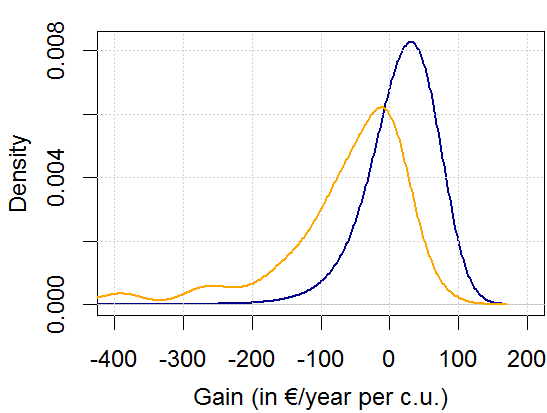
\includegraphics[width=0.28\paperwidth]{Images/pdf_transport_titled.png}
% \caption{Transport fuels}
% \end{subfigure}\hfill
% \begin{subfigure}{.3\textwidth}
% \centering
% 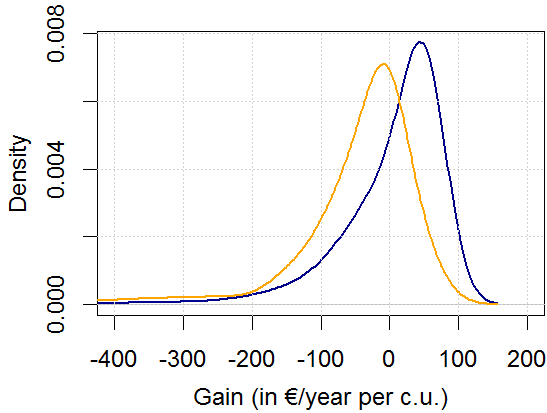
\includegraphics[width=0.28\paperwidth]{Images/pdf_housing_titled.png}
% \caption{Housing energy}
% \end{subfigure}\hfill
% \begin{subfigure}{.3\textwidth}
% \centering
% 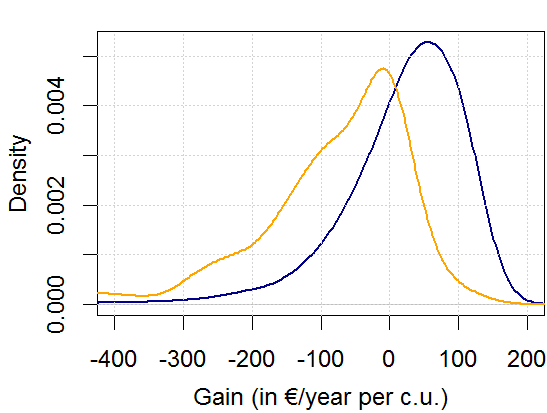
\includegraphics[width=0.28\paperwidth]{Images/pdf_carbon_tax_titled.png}
% \caption{Both}
% \end{subfigure}
% \caption{Distribution of objective (dark blue) vs. subjective (orange) net gains from our tax \& dividend.}
% \label{fig:kernel_pdf}
% \end{figure}

% -daej: remonter les CDF qui son trop bas dans le texte => le truc c'est qu'on n'a pas la maîtrise sur la mise en page AEJ, donc j'sais pas si c'est bien utile de se faire chier. Ça peut aussi attendre l'ultime révison. -> on leur envoie quand même le pdf donc il faut que ça ait une bonne tête

\vspace{-0.05in}
\begin{figure}[H]
\makebox[\textwidth][c]{
\begin{subfigure}{.3\paperwidth}
\centering
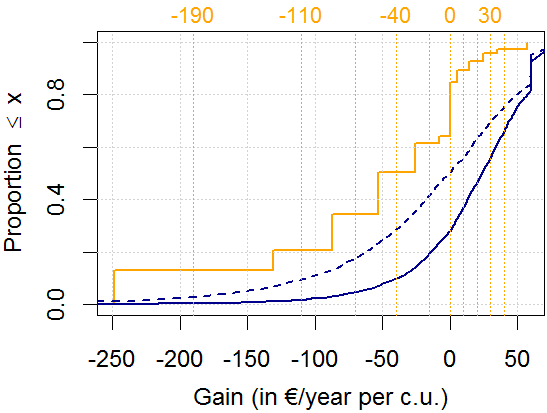
\includegraphics[width=0.28\paperwidth]{Images/cdf_transport_titled.png}
\caption{Transport fuels}
\end{subfigure}\hfill
\begin{subfigure}{.3\paperwidth}
\centering
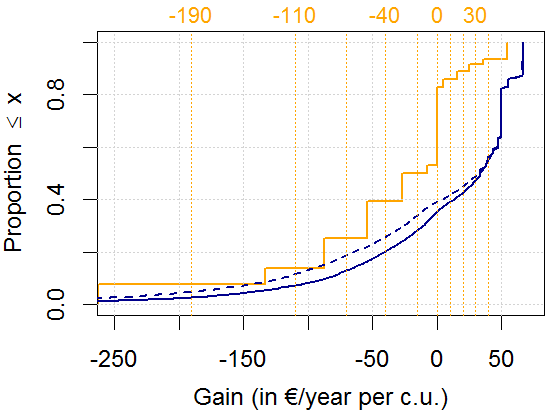
\includegraphics[width=0.28\paperwidth]{Images/cdf_housing_titled.png}
\caption{Housing energy}
\end{subfigure}\hfill
\begin{subfigure}{.3\paperwidth}
\centering
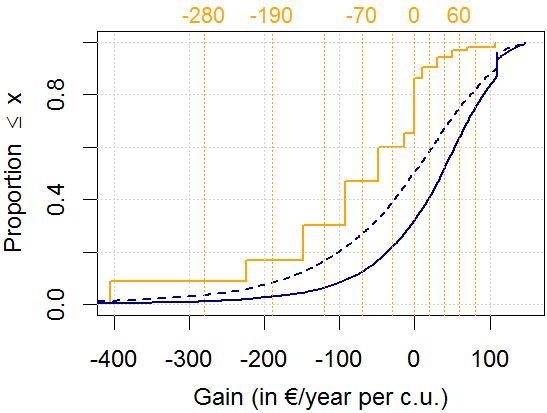
\includegraphics[width=0.28\paperwidth]{Images/cdf_carbon_tax_titled.png}
\caption{Both}
\end{subfigure}
}
\\ \quad \\  \parbox[t]{\textwidth}{\linespread{1.2}\selectfont \footnotesize{\textsc{Note:} The dashed blue lines represent the distributions of the objective gains in the extreme case of totally inelastic expenditures. The vertical dotted orange lines show the limits of the intervals of the answers to the subjective gains.}
\caption{Cumulative Density Function of objective (dark blue) vs. subjective (orange) net gains from our tax \& dividend. \label{fig:step_cdf}}}
\end{figure} %

\paragraph{Heterogeneity in bias}

%dr2 : "Ecologist" -> "Environmentalist" dans la table 3.1.

\begin{table}[!htbp] \centering 
  \caption{Determinants of bias in subjective gains.} 
  \label{tab:bias} 
\makebox[\textwidth][c]{ \begin{tabular}{@{\extracolsep{5pt}}lccc} 
\\[-1.8ex]\hline 
\hline \\[-1.8ex] 
\\[-2.8ex] & \multicolumn{3}{c}{Large bias ($\left|\widehat{\gamma}-g\right| > 110$)} \\ 
\\[-1.8ex] & \textit{OLS} & \textit{logistic} & \textit{OLS} \\ 
\hline \\[-1.8ex] 
 Initial tax: PNR (I don't know) &  &  & $-$0.179 \\ 
  &  &  & (0.023) \\ 
  Initial tax: Approves &  &  & $-$0.284 \\ 
  &  &  & (0.031) \\ 
  Yellow Vests: PNR & 0.039 & 0.035 & 0.024 \\ 
  & (0.036) & (0.035) & (0.036) \\ 
  Yellow Vests: understands & 0.081 & 0.062 & 0.041 \\ 
  & (0.025) & (0.024) & (0.025) \\ 
  Yellow Vests: supports & 0.108 & 0.103 & 0.051 \\ 
  & (0.026) & (0.025) & (0.026) \\ 
  Yellow Vests: is part & 0.202 & 0.193 & 0.147 \\ 
  & (0.048) & (0.040) & (0.047) \\ 
  Environmentalist & $-$0.064 & $-$0.061 & $-$0.025 \\ 
  & (0.026) & (0.026) & (0.026) \\ 
  Left-right: Left & $-$0.066 & $-$0.044 & $-$0.045 \\ 
  & (0.063) & (0.065) & (0.061) \\ 
  Left-right: Center & $-$0.062 & $-$0.048 & $-$0.046 \\ 
  & (0.065) & (0.068) & (0.064) \\ 
  Left-right: Right & $-$0.024 & $-$0.010 & $-$0.026 \\ 
  & (0.064) & (0.066) & (0.063) \\ 
  Left-right: Extreme-right & $-$0.076 & $-$0.057 & $-$0.088 \\ 
  & (0.066) & (0.069) & (0.065) \\ 
  Left-right: Indeterminate & $-$0.009 & 0.017 & $-$0.007 \\ 
  & (0.061) & (0.063) & (0.060) \\ 
 \hline \\[-1.8ex] 
Controls: Sociodemo, political leaning & \checkmark & \checkmark & \checkmark \\ 
Observations & 3,002 & 3,002 & 3,002 \\ 
R$^{2}$ & 0.061 &  & 0.098 \\ 
\hline 
\hline \\[-1.8ex] 
\end{tabular} 
 } {\footnotesize \parbox[t]{12cm    }{\linespread{1.2}\selectfont \textsc{Note:}  Standard errors are reported in parentheses. For the logit, the average marginal effects are reported and not the coefficients. The omitted variables are \textit{Yellow Vests: opposes} and \textit{Left-right: Extreme-left}. The list of controls can be found in the Appendix \ref{set_controls}. A large bias is defined as a difference between the subjective ($g$) and objectively estimated ($\hat{\gamma})$ net gain larger than 110\euros{}/year per c.u. }}  \end{table}

% dr2 : revoir la manière de présenter le "large bias". C'est vrai que la terminologie n'est pas précise puisqu'on emploi tantôt "misperception", tantôt "large bias" pour désigner la même chose, donc on se demande si ceux qui n'ont pas un "large bias" ont des perceptions correctes. En gros il faut remplacer "misperception" par "large bias" et adapter quelque peu le texte.

%dr2 : "the position towards the Yellow Vests appears" -> "the attitudes towards the Yellow Vests movement appear"
%dr2 : "one's position towards the policy" -> "one's attitude towards the policy"
% dr2 : préciser ce qu'on mesure avec "attitude towards the policy" (i.e. quelle question précisément). Est-ce qu'ajouter "when it is first presented" après "approve of the policy" suffit ? Ou plutôt "at the initial stage" pour que l'on voit bien que dans le diagramme ça correspond à "initial perceptions" ? => ok, done -> tu préfères pas "at the initial stage" ? C'est moins joli mais plus clair. => moi je trouvais ça plus clair "when it is first presented" justement, mais j'avais pas pensé au diagramme. On peut laisser tel quel.

% dr2: new paragraph below (misperception => large bias)
% dr2 (we regress) having a \textit{large bias} => what we call a \textit{large bias} (over many respondent characteristics)
% dr2 (A large bias is defined ...) as => . Indeed, (our estimation differs in 5% of cases) -> je comprends pas cette suggestion => Finir la phrase au lieu de "as", et mettre "Indeed". -> ok done
% dr2 (This definition ensures that the 55\% of respondents with a large bias) clearly misperceive their gains => have in fact a clear misperception. -> ou bien "This definition ensures that for the 55\% of respondents with a large bias there is a clear gap between their subjective perceptions and the actual impact of the reform." => ok. -> changé en "actual net gains" pour être plus précis
% dr2 : "Other definitions of the large bias yield very similar" -> "Other definitions yield very similar"
% dr2 : "the most critical determinant of having a large bias" -> "the most critical determinant" ?
% dr2 : "people who approve of the policy are" -> "people who approve of the policy at the initial stage are"

% sr2 : ça réduit pas beaucoup, mais on pourrait changer : "we identify several variables having a significant effect on \textit{large bias} even when controlling the false discovery rate at 5\%.\footnote{...} Environmentalists are approximately 6 p.p. less likely to display a large bias. Interestingly, while the standard left/right political leaning has no significant effect, the attitudes towards the Yellow Vests movement appear to be the most critical determinant. Relative to respondents..." -> "we identify several variables having a significant effect on \textit{large bias}---even when controlling the false discovery rate at 5\%--- such as being an environmentalist or the attitude towards the Yellow Vests movement, by contrast to the standard left/right political leaning that has no significant effect.\footnote{...} Indeed, relative to respondents..." => pk pas mais ça change quasiment rien -> on fait ce changement ou pas ? J'ai pas trop d'avis... edit?
% sr2 Environmentalists are approximately 6 p.p. less likely to display a large bias. Interestingly, while the standard left/right political leaning has no significant effect, the attitudes towards the Yellow Vests movement appear to be the most critical determinant. Relative to respondents who declared to be opposed to the movement, those who declared to ``understand'', ``support'', or ``be part'' of it are more likely to have a large bias. This effect... 
%=> Relative to respondents who declared to be opposed to the movement, those who declared to ``understand'', ``support'', or ``be part'' of the Yellow Vests are more likely to have a large bias. This effect... -> ok, le changement concerne seulement l'emplacement de Yellow Vests, la reste ne bouge pas ? => non la proposition c'est de retirer les deux phrases qui précèdent. -> ça fait perdre de l'info, notamment le ocmmentaire sur gauche/droite qui nécessite d'interpréter plusieurs coefs, je trouve ça important comme résultat. => ok. Il faudra juste réduire Section 3 à un ou deux endroits quand même. edit?
% dr2 "Environmentalists are approximately 6 p.p. less likely to display a large bias. Interestingly, while the standard left/right political leaning has no significant effect, the attitudes towards the Yellow Vests movement appear to be the most critical determinant. Relative to respondents who declared to be opposed to the movement, those who declared to ``understand'', ``support'', or ``be part'' of it are more likely to have a large bias. This effect..." 
%-> "While we find that environmentalist are less likely to display a large bias and that the standard left/right political leaning as no significant effect, the degree of support to the Yellow Vests movement is positively associated with a large bias. This effect..." => done  (edit?)

% dr2 : exemple d'endroit où on ne précise pas à quelle question on fait référence : ci-dessous on devrait préciser sur quelle question on mesure le large bias, par exemple en ajoutant "for our tax \& dividend policy" après "greater than 110\euro{} per c.u.". et il faudrait peut-être même être plus précis pour dire que c'est la perception initiale. => done. Par contre pas besoin de préciser que c'est initial je pense.

% !tr2 relire les dr2 et en rajouter certains dans la lettre à l'éditeur, notamment pour l'exposition
%!tr2 : relire et s'assurer qu'à chaque fois qu'on parle de résultats qui exploitent des questions du sondage, le lecteur puisse directement savoir à qelle séquence du sondage on fait référence.

% dr2 (edit?) : "Indeed, our estimation differs from the true objective gain by more than 110\euro{} in only 5\% of cases. This definition ensures that for the 55\% of respondents with a large bias there is a clear gap between their subjective perceptions and their actual net gains. Other definitions yield very similar results." ce passage pourrait aller en footnote si on veut réduire un peu la taille du texte de la section. => done

To characterize profiles of individuals more likely to misperceive their gains, we regress what we call a \textit{large bias} over many respondent characteristics. A large bias is defined as a gap between objectively estimated and subjective net gains greater than 110\euros{} per c.u. for our tax \& dividend policy.\footnote{Indeed, our estimation differs from the true objective gain by more than 110\euros{} in only 5\% of cases. This definition ensures that for the 55\% of respondents with a large bias, there is a clear gap between their subjective perceptions and their actual net gains. Other definitions yield very similar results.} The results given in Table \ref{tab:bias} show that having a large bias is largely idiosyncratic: when controlling for a large set of variables\footnote{The control variables used throughout the paper are described in the Appendix \ref{set_controls}.} (column 1), R$^\textnormal{2}$ remains small (0.06). Nevertheless, we identify several variables having a significant effect on \textit{large bias}, even when controlling the false discovery rate at 5\%.\footnote{To conduct the multiple testing procedure \citep[following][]{benjamini_controlling_1995}, instead of associating each dummy with a different null hypothesis, we used F-tests of joint nullity for the dummies of each categorical variable and for two additional triplets of variables: those related to household composition and those related to income.} While we find that environmentalists are less likely to display a large bias and that the standard left/right political leaning has no significant effect, the degree of support for the Yellow Vests movement is positively associated with a large bias. This effect increases with the degree of adhesion, up to 20 p.p. for individuals who reported being part of the movement. Column (3) additionally includes one's attitude towards the policy when it is first presented as a covariate. We see that people who approve of the policy at the initial stage are 28 p.p. less likely to have a large bias than those who do not accept it and 10 p.p. less likely than those who do not know.
% sr2 (voix passive) : "when it is first presented" -> "when we first present it" => je laisserais ici
% dr2: retirer la dernière phrase ("limit the speculation on reasons behind the correlations") -> oui, on n'ajoute rien à la place ? Le mini paragraphe suivant doit suffire. => oui je pense que ça suffit. Je pense que l'éditeur cherche à rendre le papier plus court, donc c'est bien d'enlever ces passages pas centraux. Old : "These results suggest that the degree of support for the policy is what most explains the bias (explaining, e.g., why \textit{Environmentalist} loses its explanatory power when we control for support) and that the Yellow Vests variables remain significant only because they capture different \textit{degrees} of rejection of the tax (which our Yes/No question cannot do)."
% sr2 passer la Table en Appendix -> pourquoi ? Le papier est déjà assez court et on la commente de manière assez extensive, c'est mieux de l'avoir sous les yeux. => ok, c'était dans l'optique de réduire la Section 3 comme demandé mais c'est vrai que c'est moins pratique. edit?

% sr2: faire plutôt le changement large bias => misperception (aussi dans la table). Ça induit beaucoup moins de changement et emploi des formulations plus naturelles, le seul défaut c'est que c'est  moins self-explanatory et notamment dans la Table, mais avec sa note ça passe. Au final je vote pour cette suggestion du coup. Ça donne ça: -> j'aime moins parce que ça sous-entend que ceux qui n'ont pas bias > 110 n'ont pas des misperceptions. => ok as you like
% To characterize profiles of individuals more likely to misperceive their gains, we regress misperception over many respondent characteristics. \textit{Misperception} is defined as a gap between objectively estimated and subjective net gains greater than 110\euro{} per c.u. as our estimation differs from the true objective gain by more than 110\euro{} in only 5\% of cases. This definition ensures that the 55\% of respondents with a misperception have in fact a large bias. Other definitions of the bias yield very similar results. The results given in Table \ref{tab:bias} show that misperception is largely idiosyncratic: when controlling for a large set of variables\footnote{The control variables used throughout the paper are described in Appendix \ref{set_controls}.} (column 1), R$^\textnormal{2}$ remains small (0.06). Nevertheless, we identify several variables having a significant effect on misperception even when controlling the false discovery rate at 5\%.\footnote{To conduct the multiple testing procedure \citep[following][]{benjamini_controlling_1995}, instead of associating each dummy to a different null hypothesis, we used F-tests of joint nullity for the dummies of each categorical variable and for two additional triplets of variables: those related to household composition and incomes.}. Environmentalists are approximately 6 p.p. less likely to display a misperception. Interestingly, while the standard left/right political leaning has no significant effect, the attitudes towards the Yellow Vests movement appear to be the most critical determinant of misperception. Relative to respondents who declared to be opposed to the movement, those who declared to ``understand'', ``support'', or ``be part'' of it are more likely to misperceive their gains. This effect increases with the degree of adhesion, up to 20 p.p. for individuals who reported being part of the movement. Column (3) additionally includes one's attitude towards the policy when it is first presented as a covariate: we see that people who approve of the policy are 28 p.p. less likely to misperceive their gains than those who do not accept it and 10 p.p. less likely than those who do not know. These results suggest that the degree of support for the policy is what most explains the misperception (explaining, e.g., why \textit{Environmentalist} loses its explanatory power when we control for support) and that the Yellow Vests variables remain significant only because they capture different \textit{degrees} of rejection of the tax (which our Yes/No question cannot do).

% old: To characterize profiles of individuals more likely to misperceive their gains, we regress misperception over many respondent characteristics. Misperception is defined as a gap between objectively estimated and subjective net gains greater than 110\euro{} per c.u. because our estimation differs from the true objective gain by more than 110\euro{} in only 5\% of cases. This definition ensures that 55\% of respondents with a misperception have in fact a large bias. Other definitions of the bias yield very similar results. The results given in Table \ref{tab:bias} show that misperception is largely idiosyncratic: when controlling for a large set of variables\footnote{The control variables used throughout the paper are described in Appendix \ref{set_controls}.} (column 1), R$^\textnormal{2}$ remains small (0.06). Nevertheless, we identify several variables having a significant effect on misperception even when controlling the false discovery rate at 5\%.\footnote{To conduct the multiple testing procedure \citep[following][]{benjamini_controlling_1995}, instead of associating each dummy to a different null hypothesis, we used F-tests of joint nullity for the dummies of each categorical variable and for two additional triplets of variables: those related to household composition and incomes.}. Environmentalists are approximately 6 p.p. less likely to display a large bias. Interestingly, while the standard left/right political leaning has no significant effect, the attitudes towards the Yellow Vests movement appear to be the most critical determinant of misperception. Relative to respondents who declared to be opposed to the movement, those who declared to ``understand'', ``support'', or ``be part'' of it are more likely to misperceive their gains. This effect increases with the degree of adhesion, up to 20 p.p. for individuals who reported being part of the movement. Column (3) additionally includes one's attitude towards the policy when it is first presented as a covariate: we see that people who approve of the policy are 28 p.p. less likely to misperceive their gains than those who do not accept it and 10 p.p. less likely than those who do not know. These results suggest that the degree of support for the policy is what most explains the bias (explaining, e.g., why \textit{Environmentalist} loses its explanatory power when we control for support) and that the Yellow Vests variables remain significant only because they capture different \textit{degrees} of rejection of the tax (which our Yes/No question cannot do).

%dr2 : "EDITOR'S NOTE:" ci dessous déplacée pour éviter un espèce de saut de paragraphe introduit avant Environmentalist.
 %%EDITOR'S NOTE: Please ensure that the intended meaning has been maintained in this edit. % sss Not sure if the meaning has been maintained. The idea is that we make sure the false discovery rate stays below 5%: it is not equal to 5%. Wikipedia says: "The Benjamini–Hochberg procedure (BH step-up procedure) controls the FDR at level alpha" where level alpha is our 5% (https://en.wikipedia.org/wiki/False_discovery_rate) %% RCP NOTE: Edited to revert to the original.
% sss If we change "We can think" by "We argue" (that the degree of support...), we should also change "what determines most of the bias". Because the bias is largely idiosyncratic, and although policy support is the biggest determinant, it still explains a low share of the variance. So maybe replace "what determines most of the bias" by "what most explains the bias"? (and/or replace "We argue" by "These results suggest") %% RCP NOTE: Edited. => saej je propose qu'on fasse aussi le changement "what most explains the bias" -> ok => done daej

% dr2 : change "typical biases" qui n'est pas clair -> peut-être simplement supprimer "typical" ? Ou écrire "respondents' biases" ? => done, typical enlevé
% dr2 : l'éditeur signale que "because" ne va pas parce qu'on ne montre rien de causal sur les croyances. Est-ce que si on remplace "provides evidence" par "provides correlational evidence" ça suffit ? Ou on change complètement la formulation ? => remplacer "provides evidence" par "suggest"? -> c'est peut-être trop faible "suggest" sachant qu'on montre des résultats non ? Ou "provides non-causal evidence suggesting that" ? => pour moi le pb est pas la causalité, mais le fait qu'il y a d'autres interprétations (confiance recevoir dividende), donc je dirais plutôt "suggest". -> Sinon on peut aussi être moins spécifique en disant "Section \ref{sec:persistence} provides evidence suggesting that people form their beliefs differently depending on their attitude towards the tax, ...". Ca permet d'enlever le "because" qui est trp fort, et c'est plus général parce que ça spécifie pas le mécanisme. => mouais si tu veux. C'est un peu un oxymore evidence suggesting mais ça peut passer -> Sinon "The results of Section \ref{sec:persistence} suggest that..." => ok

% old : Section \ref{sec:persistence} provides evidence that some people think that they will lose because they oppose the tax, while Section \ref{sec:motives5} shows that perceived outcomes causally influence support.

% sr2: reformuler pour éviter de mettre en avant MR (a minima par ex "their attitude towards the tax" => "their political views and identity" -> j'ai remplacé). Je propose aussi de changer "rejection" par "attitude towards the policy" qui est plus précis. => ok done -> on considère que c'est suffisant comme changements ? => oui
Overall, the biases are large and closely related to one's convictions. However, the direction(s) of the causality between beliefs and attitude towards the policy is not resolved at this stage. The results of Section \ref{sec:persistence} suggest that people form their beliefs differently depending on their political views and identity, while Section \ref{sec:motives5} shows that perceived outcomes causally influence support.

\subsection{Environmental effectiveness\label{subsec:perception_ee}}

A well-established result in the literature on the acceptability of climate policies is the perceived ineffectiveness of Pigouvian instruments \citep[e.g.,][]{dresner_social_2006,kallbekken_et_al_2011, baranzini_effectiveness_2017}. In particular, people do not see carbon taxes as effective in combating climate change. Our findings confirm this result. Among the respondents who did not receive the information on environmental effectiveness, only 15\% answered ``Yes'' when asked whether our tax \& dividend would be effective in reducing pollution and fighting climate change, 68\% answered ``No'' and 18\% answered that they did not know.

% sr2 (voix passive) : "when asked whether our" -> "when we asked whether our" => je laisserais -> il faudrait demander à un natif, c'est peut-être un peu bizarre "when aksed" => AJE

% dr2 : préciser le sample pour le résultat ci dessus (je ne comprends pas trop d'où vient la confusion). Peut-être que c'est "among" qui crée de la confusion ? Dans ce cas on pourrait écrire "confirm this result: only 17\% of our survey respondents answered ``Yes''..." après quoi je ne vois plus trop d'ambiguité possible. On peut aussi mettre "of our 3,002 survey respondents" pour q'uil y ait aucune ambiguité mais c'est un peu lourd. => ok, les deux me vont. Done premier changement, en enlevant "our survey" -> je trouve qu'en enlevant "our survey" on n'a pas beaucoup clarifié par rapport à son commentaire. => Sinon on revient à l'ancienne et on dit "among the 3,002 respondents" -> ou bien "only 17\% of the 3,002 respondents of our survey answered..." ? c'est un peu bizarre de dire 3,002 sans préciser que c'est notre survey. => on peut mettre "among our 3,002 respondents" alors -> ok j'ajoute seulement ça, done. => en fait ce qui n'allait pas c'est le choix de parler des 3,002. Je pense qu'il faut faire ce qu'il attend: donner la stat pour ceux qui n'ont pas eu l'info (pareil pour progressivité). -> oui c'est vrai que c'est une stat plus facile à interpréter parce que ça dépend pas de la part de gens qui ont eu l'info. => j'ai changé en ce sens

%dr2 : ci-dessous, clarifier la manière dont on calcule deux élasticités prix séparées. Je propose de ré-écrire le paragraphe comme suit : "An explanation sometimes encountered to explain perceptions of ineffectiveness is that most people believe that energy consumption is quite inelastic \citep{kallbekken_saelen_2011,carattini_overcoming_2018}. In our survey, we randomly elicited respondents' perceived price elasticity of either housing or transport energy for French people. To see how perceived elasticity relates to the perception of effectiveness, we run two separate regressions where the dependent variable $E$ is equal to 0 if the respondent does not perceive the policy as environmentally effective and 1 otherwise. In the first regression, we regress the perceived effectiveness on the perceived elasticity for housing, and in the second we regress it on the perceived elasticity for transport energy. Table \ref{table:elasticities_effectiveness} in Appendix \ref{subsec:app_perception_ee} reports the results with and without control variables." => c'est juste pour le début du paragraphe hein ? Après on reprend à They all consistently..? si oui ça me va -> oui c'est bien ça, done.

%dr2 : "reduced to small" -> "attributed to small"

% old : An explanation sometimes encountered to explain perceptions of ineffectiveness is that most people believe that energy consumption is quite inelastic \citep{kallbekken_saelen_2011,carattini_overcoming_2018}. To test this hypothesis, we regress a binary variable $E$ equal to 0 if the respondent does not perceive the policy as environmentally effective and 1 otherwise on their subjective price elasticity for French people. As respondents were randomly assigned to transport or housing, we run a separate regression for both types of energy. Table \ref{table:elasticities_effectiveness} in Appendix \ref{subsec:app_perception_ee} reports the results with and without control variables. 

% dr2 : "as a respondent anticipating" -> on pourrait préciser en disant "as for both sectors a respondent anticipating". Mais peut-être que formulé ainsi ça crée plus de confusion qu'autre chose. C'est juste que ça n'a rien d'évidentq ue le résultat soit le même pour housing et transport, ça mériterait d'être un peu mis en valeur. => pourquoi pas, je pense que ça clarifie plus que ça n'ajoute de la confusion. Mais bon pas indispensable vu que c'est pas deamdné. -> ajouté (il nous demande de faire des modifs en plus de ces suggestions, toujours bon à prendre pour montrer qu'on a bossé ^^).

% dr2 si on veut raccourcir la section 3, passer à partir de To see ... jusqu'à la fin du paragraphe en Appendix, et remplacer par: We find a significant effects of perceived elasticities on perceived environmental effectiveness. However, these effects are too modest to explain the perceived ineffectiveness (see Appendix \ref{subsec:app_perception_ee}. Indeed, among respondents who perceive the policy to be environmentally ineffective, almost half anticipate responses to price changes larger than those in the literature. -> pourquoi pas, j'ai peur que le papier devienne un peu court => faut ptet pas faire toutes les modifs que je propose pour réduire la Section 3, mais au moins une ou deux je pense, qu'on puisse dire à l'éditeur qu'on a réduit comme demandé -> ce changement là est peut-être celui qui nous coûte le moins, on peut déjà l'adopter. La seule chose qui me gène c'est le "Indeed, ..." parce qu'on pourrait avoir l'impression que notre analyse se limite à ça. => For instance ou For example à la place de Indeed? -> "we find significant effects" n'est peut-être pas assez précis, et surtout il risque de nous reprocher de ne pas préciser que ces effets ne sont pas causaux (ce que significant effect pourrait suggérer). On pourrait écrire : "We find that higher perceived elasticities are more often associated with the belief that the policy is effective, even when controlling for many respondents' characteristics." comme ça on voit qu'on utilise des régressions avec contrôle, et on peut garder la suite comme c'est. => ok done. Je me demande si on devrait pas enlever "more often" -> on perdrait en précision non ? ou alors "are associated with a higher likelihood to believe that", ou simplement "are more likely associated" ? => done first
An explanation sometimes encountered to explain perceptions of ineffectiveness is that most people believe that energy consumption is quite inelastic \citep{kallbekken_saelen_2011,carattini_overcoming_2018}. In our survey, we randomly elicited respondents' perceived price elasticity of either housing or transport energy for French people. We find that higher perceived elasticities are associated with a higher likelihood to believe that the policy is effective, even when controlling for many respondents' characteristics. However, these effects are too modest to explain the perceived ineffectiveness (see Appendix \ref{subsec:app_perception_ee}). Indeed, among respondents who perceive the policy to be environmentally ineffective, almost half anticipate responses to price changes larger than those in the literature.\footnote{Overall, the average subjective elasticities are close to the estimates of the literature for transport (at $-$0.45) and somewhat overestimated for housing ($-$0.43). Among those who declared that the policy was not effective, 45\% (resp. 43\%) anticipated an aggregate elasticity at or below $-$0.5 for housing (resp. for transport), while elasticities obtained from the literature are approximately $-$0.2 for housing and $-$0.4 for transport.\label{fnel}}

% dr2 : "a significant effects" -> choisir entre singulier et pluriel. j'enleverais le "a".

%  "To see how perceived elasticity relates to the perception of effectiveness, we run two separate regressions where the dependent variable $E$ is equal to 0 if the respondent does not perceive the policy as environmentally effective and 1 otherwise. In the first regression, we regress the perceived effectiveness on the perceived elasticity for housing, and in the second we regress it on the perceived elasticity for transport energy. Table \ref{table:elasticities_effectiveness} in Appendix \ref{subsec:app_perception_ee} reports the results with and without control variables. They all consistently indicate that perceived elasticities are correlated with beliefs about the policy's effectiveness, as for both sectors a respondent anticipating an elasticity of $-$1 is (on average) 6 p.p. more likely to perceive the policy to be effective than one anticipating no elasticity. Although significant, the magnitude of the effect is modest, showing that the perceived ineffectiveness of tax instruments should not be attributed to small subjective elasticities." -> basculé en appendix



%dr2 : "close to these estimates" -> "close to the estimates of the literature"

% dr2 ptet condenser aussi ce paragraphe -> on pourrait déjà supprimer "and is only... in 2050". => done, ptet aussi le 0.01% of global l emissions. Removed: and is only a small step towards the official objective of carbon neutrality in 2050 -> dans la perspective de lutter contre le changement climatique, la comparaison aux émissions mondiales a plus de sens, donc je trouve ça plutôt bien de le garder.
% dr2 : "BdF data" could be "official data", "Insee data", or as you suggested in the pdf "Insee (BdF) data" that I like less because it is not only BdF but the combined dataset. => done. official data
% dr2 : "according to the simulation from official data" -> pourrait basculer dans la footnote qui suit ("The computations are based...") pour réduire un peu la taille du texte. => done

% dr2 : "the tax should reduce" -> "our tax \& dividend policy should reduce", to be more specific as asked by the editor.
A more plausible explanation for perceived ineffectiveness is that people do not believe that the policy would be sufficient to \textit{substantially} affect pollution and climate change. Taking respondents' average anticipated elasticities for transport and housing energy (that are fairly accurate\footref{fnel}), our tax \& dividend policy should reduce French greenhouse gas (GHG) emissions by 5.7 Mt of CO$_\textnormal{2}$ equivalents (CO$_\textnormal{2}$e) each year. This reduction corresponds to 0.8\% of French annual emissions and 0.01\% of global emissions.\footnote{The computations are based on household carbon emissions simulated from official data. In 2014, French GHG consumption-based emissions were equal to 712 MtCO$_\textnormal{2}$e \citep{cgdd_chiffres_2019}. In 2017, global emissions were 53.5 GtCO$_\textnormal{2}$e \citep{unep_emissions_2018}.} Thus, although respondents do anticipate responses to price incentives, our results suggest that they do not perceive a 50\euro{}/tCO$_\textnormal{2}$ national carbon tax to be a proportionate reaction to climate change.

\subsection{Progressivity\label{subsec:beliefs_progressivity}}
% sss "wealthier" changes the meaning of "richer": we are talking about income, not wealth %% RCP NOTE: Edited.
% dr2 (edit?) : passer les 3 premières phrases (avec toutes les citations) dans une footnote à la fin du paragraphe. (je suis pas fan mais c'est si on veut "keep this [section] relatively short" comme Luttmer nous dit). -> ça ferait vraiment court comme sous-section non ? => oui c'est pas la façon de réduire la Section 3 que je préfère -> Je propose une version plus soft de ce changement en remplaçant "A broad literature has shown that carbon taxation alone is regressive \citep{poterba_is_1991,metcalf_distributional_1999,grainger_who_2010}, meaning that it is more costly for poorer households as a share of their resources. However, it has also been shown that redistributing its revenue through..." par "However, the literature has shown that redistributing the revenue of a carbon tax through..." => ok done, on drop 3 citations du coup ? -> oui je pense que c'est pas très grave, c'est des papiers à citer sur les effets redistributifs mais c'est pas fondamental dans notre cas
It is often argued that a critical barrier to the acceptance of carbon taxation is its perceived distributional impact, in particular the higher burden imposed on lower income households \citep{bristow_public_2010,brannlund_tax_2012,gevrek_public_2015}. However, the literature has shown that redistributing the revenue of a carbon tax through uniform lump-sum transfers---i.e., a tax \& dividend---can make the policy progressive \citep{west_williams_04,bento_distributional_2009,williams_initial_2015}, including for France \citep{bureau_distributional_2011,douenne_2020}. Figure \ref{figure:effort_rate_uc} in Appendix \ref{subsec:app_distributive} displays the average net gain by income decile for our tax \& dividend. This figure shows that lower income households would gain more than richer households, both in relative and in absolute terms. However, among respondents who did not receive the information on the progressivity, only 19\% of respondents think the policy would benefit the poorest households, compared to 60\% who declare that it would not and 20\% who do not know.

%dr2 : "It clearly appears from this figure" -> "This figure shows"

% dr2 : modifier les résultats sur le sous-échantillon de ceux n'ayant pas eu l'info progressivité, et le préciser. => done, ajouté: among respondents who did not receive the information on the progressivity, (et changé pourcentaes)

% dr2 : modifier le titre de cette section pour montrer que l'on étudie l'ensemble des déterminants des beliefs, et non seulement les attitudes. L'éditeur suggère "Predictors of beliefs" ou "Effects on beliefs". "Predictors of belies" me convient même si je ne suis pas non plus totalement convaincu, pas le deuxième. Une autre idée ? => "Determinants of beliefs"? -> c'est peut-être le mieux oui. => done (was How attitudes shape beliefs)
\section{Determinants of beliefs \label{sec:persistence}}

% sr2 : "views simply reflected" -> "views simply reflect" ?
% dr2  (voix passive): "to assess how beliefs are formed." -> "tp assess how beliefs form" ou "to assess how people form their beliefs". => done second
% dr2 (voix passive) : "after new information is provided," -> "after they receive new information" ou "after we provided new information" => done first

The previous section has shown that people's low acceptance of our tax \& dividend correlates with pessimistic beliefs about the properties of the scheme. As knowledge about these properties has been shown to be decisive for acceptance \citep{carattini_overcoming_2018}, it is important to assess how people form their beliefs. In the following, we test respondents' reactions to information about their gains, environmental effectiveness, and progressivity. If overly pessimistic views simply reflected a lack of knowledge, we would expect them to revise their beliefs after they receive new information, which is what we refer to as ``updating''. %

\subsection{Self-interest}\label{subsec:update_si}

\subsubsection{Pessimism in the revision of beliefs\label{subsubsec:update_after_feedback}} %

% dr2 add (the \textit{ex post} belief is on average consistent with the fact that 83\% of them do in reality lose from the tax \& dividend policy), with 86\% endorsing our ``lose'' feedback. -> done  
Our respondent-specific estimation of net gains (see Section \ref{subsec:Households-surveys}) enables us to tell respondents that given their characteristics, they have a 5-in-6 chance to ``win'' or ``lose'' from the policy. We can then examine how they update their beliefs about their win/lose category after receiving this information. The full transition matrices of people's beliefs are given in Tables \ref{table:transition_matrix_positive_feedback} and \ref{table:transition_matrix_negative_feedback} in the Appendix \ref{subsec:app_perception_si}. More concisely, Table \ref{table:confidence_intervals_beliefs_feedback} reports the share of respondents whose beliefs after being informed are aligned with our feedback with the corresponding 95\% binomial confidence intervals. It shows a highly asymmetric response depending on the feedback received. On the one hand, for the 24\% of individuals who receive ``lose'' feedback $(\widehat{\Gamma} = 0)$, the \textit{ex post} belief is on average consistent with the fact that 83\% of them do in reality lose from the tax \& dividend policy, with 86\% endorsing our ``lose'' feedback. If anything, these people would rather tend to \textit{agree too much} with our noisy signal, especially when excluding people who initially consider themselves to be unaffected (i.e., focusing on $g^0 \neq 0$). On the other hand, the 76\% who received ``win'' feedback $(\widehat{\Gamma} = 1)$ appear to be much more conservative in their revision since only 25\% of them endorse the ``win'' feedback. Among the respondents who initially thought that they would lose in this group, a mere 12\% switch their answer from ``lose'' to ``win''. This is in sharp contrast to the respondents who initially thought they would win and receive ``lose'' feedback since 82\% of them endorse our prediction. Thus, pessimistic beliefs are consistent with our treatment, but optimistic beliefs are not.

%dr2 : "are effectively losers." -> "do in reality lose from the tax \& dividend policy".

\begin{table}[!htbp] \centering 
  \caption{Share of respondents with new beliefs aligned with feedback.}
  \vspace{-0.5cm}
  \label{table:confidence_intervals_beliefs_feedback} 
\begin{tabular}{@{\extracolsep{5pt}}lcc} 
\\[-1.8ex]\hline 
\hline \\[-1.8ex] 
 & \multicolumn{2}{c}{\textit{Aligned with feedback: $G^F = \widehat{\Gamma}$}} \\ 
\cline{2-3} 
\\[-1.8ex]
 & \multicolumn{2}{c}{Feedback:}
\\ & win $(\widehat{\Gamma} = 1)$ & lose $(\widehat{\Gamma} = 0)$ \\ \vspace*{0.5cm} & (75.8\%)  & (24.2\%) \\ \hline \\[-1.8ex] 
 Initial belief winner ($g^0 > 0$) & 78.8\% & 81.5\% \\ 
 (14.0\%) & {\small $\left[73.2\% ; 83.4\%\right]$} & {\small $\left[65.0\% ; 91.3\%\right]$} \\ 
 Initial belief unaffected ($g^0 = 0$) & 21.6\% & 44.9\% \\ 
 (21.7\%) & {\small $\left[17.6\% ; 26.2\%\right]$} & {\small $\left[33.5\% ; 56.8\%\right]$} \\ 
 Initial belief loser ($g^0 < 0$) & 12.2\% & 93.9\% \\ 
 (64.3\%) & {\small $\left[10.3\% ; 14.5\%\right]$} & {\small $\left[90.9\% ; 96.0\%\right]$} \\ 
 Initial belief affected ($g^0 \neq 0$) & 26.1\% & 92.9\% \\ 
 (78.3\%) & {\small $\left[23.7\% ; 28.7\%\right]$} & {\small $\left[89.8\% ; 95.1\%\right]$} \\ 
  & & \\
  [-1.8ex] \hline \\[-1.8ex]
 All & 25.1\% & 85.7\% \\ 
 (100\%) & {\small $\left[23.0\% ; 27.3\%\right]$} & {\small $\left[82.2\% ; 88.7\%\right]$} \\
 & & \\
 [-1.8ex]\hline 
\hline \\[-1.8ex]
\end{tabular}
{
\\ %
\footnotesize \parbox[t]{14cm}{\linespread{1.2}\selectfont \textsc{Note:} The 95\% confidence intervals for the binomial probabilities are given in brackets. The Table reads as follows: among those who initially think that they would win ($g^0 > 0$) but are told that they are expected to lose ($\hat{\Gamma} = 0$), 81.5\% agree that they would lose ($G^F = 0$). The feedback $\hat{\Gamma}$ is not a random draw but a deterministic outcome of the characteristics reported by the respondents in the survey. The subsample used is the 1,968 respondents who received feedback.}}
\end{table}
% dr2 : give the sample size in the note above. => il demande quel est l'échantillon, pas sa taille. On peut ptet refuser de faire ce changement? sinon on remplace le (100\%) par (100\%, i.e. 3,002 respondents) dans la table. -> pourquoi tu voudrais refuser ? Il n'y a pas 3,002 ici puisque tout le monde ne reçoit pas le feedback. => awi^^ du coup on peut rajouter une phrase à la fin de la note: The subsample used are the 1,968 respondents who received a feedback. -> ok done, même si ça fait beaucoup cette note.

Table \ref{table:confidence_intervals_beliefs_feedback_biased} in the Appendix \ref{subsec:app_perception_si} conducts the same analysis for the 28\% of respondents whose gain is very positive or very negative, i.e., above 110\euros{} per c.u. in absolute terms. For these respondents, our out-of-sample prediction of the win/lose category is correct in 99\% of the cases, as seen in Figure \ref{fig:proba_pred} in the Appendix \ref{subsec:app_perception_si}. The alignments with our feedback are similar between the whole sample and these respondents for whom we are certain to make a correct prediction. The similarity of alignments for different prediction accuracies rules out the possibility that a large fraction of respondents do not update their beliefs because their private information would be \textit{truly} more accurate than our prediction.

\subsubsection{Causal effect of feedback on beliefs\label{subsec:causal_feedback}} 
% dr2 La transition avec ce qui précède me paraît imparfaite. Je propose: In order to be relevant, our feedback on respondents' win/lose category had to be customized and as accurate as possible. This information intervention is therefore not a randomized treatment and we cannot simply compare the \textit{ex post} belief of those who received a \textit{win} vs. \textit{lose} feedback as coming from two otherwise identical groups. Despite this non-random assignment of the treatment, there is still a way to estimate the causal effect => While we have just analyzed the effect of providing \textit{information} about the respondents' net gains on their win/lose belief, we have yet to compare the effect of receiving a \textit{win} vs. \textit{lose} feedback for a given respondent. Despite the non-randomness of our feedback, there is a way to estimate the causal effect -> je ne suis pas fan de la première phrase qui je trouve ne fait pas une claire distinction entre ces deux sections. Je propose : "In order to be relevant, our feedback on respondents' win/lose category had to be customized and as accurate as possible. This information intervention is therefore not a randomized treatment and we have not identified its causal effect on respondents' beliefs. Despite this non-random assignment..." => "As our information intervention was not a randomized treatment, we have yet to identify the causal effect of receiving a \textit{win} vs. \textit{lose} feedback on respondents' beliefs. Despite the non-random assignment..."? En fait ce qui me gène avec ta version c'est que dans 4.1.1 pour moi on identifie un effet causal : celui d'apporter de l'information. C'est pas l'effet causal de win vs. lose par contre, qu'on traite mtn. -> ok pour ta proposition, même si je pense qu'on pourrait garder la première phrase qu'on a actuellement. => ok done en la gardant

% dr2 : "in a regression discontinuity design (RDD)" -> "in a RDD" (c'est déjà défini page 4).

To be relevant, our feedback on respondents' win/lose category had to be customized and as accurate as possible. Since our information intervention was not a randomized treatment, we have yet to identify the causal effect of receiving \textit{win} vs. \textit{lose} feedback on respondents' beliefs. Despite this non-random assignment of the treatment, there is still a way to estimate the causal effect of the feedback on people's beliefs. The binary win/lose feedback is a variable $\widehat{\Gamma}$ that jumps from 0 to 1 when our continuous estimation of respondents' net gains $\widehat{\gamma}$ exceeds the zero threshold. The following equation enables us to estimate the threshold effect around zero net gain in an RDD, and thus to obtain the effect of receiving \textit{win} compared to \textit{lose} feedback:


\begin{equation}
    G_i^F = \alpha_0 + \alpha_1 \widehat{\Gamma}_{i} + \alpha_{\gamma,1} \widehat{\gamma}_{i} + \alpha_{\gamma,2} \widehat{\gamma}_{i}^{\;2} + \mathbf{\alpha_C C_i} + \mathbf{\alpha_I I_i} + \eta_i
    \label{eq:effect_feedback}
\end{equation}

The dependent variable $G^F$ represents respondents' belief about their gain after the feedback. It is equal to 0 if they believe they lose, and 1 otherwise. $\mathbf{C}$ is a set of respondents' characteristics, and $\mathbf{I}$ a set of variables describing their household's income. The two terms $\widehat{\gamma}$ and $\widehat{\gamma}^{\;2}$ allow for a quadratic specification to control for estimated net gains to properly isolate the effect of receiving positive rather than negative feedback. To better identify the threshold effect in the RDD, we focus on the subsample of respondents whose estimated net gain $\widehat{\gamma}$ is close to zero (less than 50\euros{} per annum in absolute value). Table \ref{tab:effect_feedback} displays the results, including our main specification (column 1), the same estimation performed on the full sample (2), a modified version of (1) where interaction terms have been added to study heterogeneous treatment effects (3), and a specification where the dependent variable corresponds to the belief to \textit{win} instead of to \textit{not lose} (4).

% !tr2 afficher gamma * g?
\begin{table}[!htbp] \centering 
  \caption{Effect feedback on belief of winning.} 
  \label{tab:effect_feedback} 
\makebox[\textwidth][c]{ \begin{tabular}{@{\extracolsep{5pt}}lcccc} 
\\[-1.8ex]\hline 
\hline \\[-1.8ex] 
\\[-1.8ex] & \multicolumn{3}{c}{Believes does not lose} & Believes wins \\ 
\\[-1.8ex] & (1) & (2) & (3) & (4)\\ 
\hline \\[-1.8ex] 
 Predicted winner ($\widehat{\Gamma}$) & 0.269 & 0.208 & 0.246 & 0.153 \\ 
  & (0.058) & (0.035) & (0.064) & (0.045) \\ 
  Initial tax Acceptance ($A^0$) & 0.306 & 0.331 & 0.015 & 0.310 \\ 
  & (0.066) & (0.038) & (0.087) & (0.051) \\ 
  Yellow Vests supporter &  &  & 0.019 &  \\ 
  &  &  & (0.058) &  \\ 
  $\widehat{\Gamma} \times A^0$ &  &  & 0.166 &  \\ 
  &  &  & (0.079) &  \\ 
  $\widehat{\Gamma} \times$ Yellow Vests supporter &  &  & $-$0.151 &  \\ 
  &  &  & (0.069) &  \\ 
  $\widehat{\Gamma} \times G$ &  &  & 0.080 &  \\ 
  &  &  & (0.079) &  \\ 
 \hline \\[-1.8ex] 
Controls: Incomes (piecewise continuous) &  \checkmark &  \checkmark &  \checkmark & \checkmark \\ 
\quad estimated gains, sociodemo, other motives  &  &  &  &  \\ 
Controls: initial win/lose category ($G$) &  &  &  \checkmark &  \\ 
Sub-sample & $\left| \widehat{\gamma}\right|<50$ &  & $\left| \widehat{\gamma}\right|<50$ & $\left| \widehat{\gamma}\right|<50$ \\ 
Observations & 757 & 1,968 & 757 & 757 \\ 
R$^{2}$ & 0.301 & 0.320 & 0.419 & 0.253 \\ 
\hline 
\hline \\[-1.8ex] 
\end{tabular} 
} {\footnotesize \parbox[t]{\textwidth}{\linespread{1.2}\selectfont \textsc{Note:} Standard errors are reported in parentheses. The list of controls can be found in the Appendix \ref{set_controls}.} }\end{table} 

Everything else being equal, after receiving the feedback, respondents predicted winners are 27 p.p. more likely to believe they do not lose than respondents predicted losers (column 1). They are also 15 p.p. more likely to believe that they win (column 4). Interestingly, column 3 shows that the effect of the informational treatment is heterogeneous. From the two interaction terms, we see that among the respondents who initially accepted the tax \& dividend policy---i.e., when it was first presented---the effect of the \textit{win} feedback on the belief not to lose goes from 27 p.p. to 41 p.p., while for those supportive of the Yellow Vests---who declared to be part of or to support the movement---it goes down to less than 10 p.p. Thus, the information provided to respondents is processed differently depending on their attitude towards the policy. While the treatment is rather effective at convincing those most favorable to the policy about its impact on their household, those most opposed to it do not appear to be receptive to this information.

\subsubsection{Mechanisms \label{sec:mechanisms}}

% dr2 pessimistic beliefs and attitudes => pessimistic and heterogeneous beliefs -> ok => ah je proposais "beliefs and attitudes => beliefs" aussi, pour éviter deux "and" -> ok ça me va, done
There are several ways to rationalize pessimistic and heterogeneous beliefs against the tax \& dividend. We propose the following four mechanisms: distrust, uncertainty, motivated reasoning, and intentional misreporting.

\paragraph{Distrust}

The first mechanism is that respondents distrust what we present to them. They may perceive our information to be biased, think that we wrongly estimated their likelihood of winning and that we are overly optimistic.\footnote{Another possibility is that respondents give too much value to their private information relative to the base rate information. That is, pessimistic winners might be overconfident in seeing themselves as specific so that they partly discard the new information, e.g., by thinking that they are part of the one-sixth for whom our prediction is erroneous, perhaps because they believe that they always lose more than others from new policies.} As a result, they may discount our new information relative to their prior information or assign relatively more weight to our information when it is pessimistic. This distrust may stem from an impression that experts understate the costs of a carbon tax or that the government will break its promise to pay the dividend. For instance, \cite{sapienza_zingales_2013} report that 51\% of Americans are skeptical that their governments would deliver on using the proceeds of a carbon tax to reduce other taxes \citep[see also][]{dresner_social_2006,hsu_pollution_2008}. A similar level of skepticism regarding the dividend could explain much of the pessimism about net gains.

\paragraph{Uncertainty}

The second mechanism stems from people's uncertainty regarding their gain. That uncertainty would make them see their possible gain as a distribution \citep[see][]{stiglitz_addressing_2019}. Then, instead of reporting the average of this distribution, loss adverse people would conservatively estimate their gains. Also, the effect of uncertainty on updating is ambiguous. On the one hand, uncertain people could be more likely to rely on our base rate information; but on the other hand, their subjective probability of losing could remain high despite our information.%

% sss => We'd prefer "Also" (as before) (or perhaps "Besides") to "Additionally": the sentence it introduces is quite unrelated to the previous one. %% RCP NOTE: Edited.

\paragraph{Motivated reasoning}

% dr2 added: "By analyzing ..." after \citep{kahan_ideology_2013}. -> très bien !

% dr2 : ajout de "even controlling for their prior belief"
The third mechanism to explain the observed asymmetry in belief revision is that some people have a strong skeptical attitude towards the carbon tax, which affects the formation of their beliefs. They would engage in motivated reasoning, i.e., update their beliefs in a way that is consistent with their initial views \citep{druckman_evidence_2019,little_distortion_2019} rather than integrate information in a way that leads to accurate conclusions. Although distrust is linked to motivated reasoning since it also involves neglecting information, in the case of distrust, people discard information because they do not trust its source; for motivated reasoning, they dismiss the information when its content contradicts preexisting views. Motivated reasoning entails a deviation from Bayesian updating---contrary to the first two mechanisms---but it can still be \textit{rationalized} as a psychological adaptation to preserve one's sense of identity \citep{kahan_ideology_2013}. By analyzing the determinants of a correct update, the online Appendix \ref{sec:heterogeneity_update} shows that those who initially disapprove of the tax \& dividend and those who are part of the Yellow Vests movement are significantly less likely to correctly update their win/lose belief after feedback (by 18 and 14 p.p., respectively), even controlling for their prior belief. This finding is consistent with motivated reasoning since political views and identity are correlated with the way people form their beliefs (see the online Appendix \ref{sec:MR} for a discussion). However, we did not demonstrated the causality, and this correlation could also stem from higher distrust (or higher uncertainty) among these groups.

% dr2 (voix passive) : "in the case of distrust, information is discarded because its source is not trusted, while for motivated reasoning, information is dismissed when its content contradicts preexisting views." -> "in the case of distrust, people discard information because they do not trust its source, while for motivated reasoning, they dismiss the information when its content contradicts preexisting views."
% dr2 (voix passive) : "the way beliefs are formed" -> "the way people form their beliefs" ou "the way beliefs form". => done first
% dr2 (voix passive) : "However, we did not demonstrated the causality, and"

\paragraph{Intentional misreporting}

A fourth possibility is that some respondents intentionally report overly pessimistic beliefs compared to what they actually think. This could stem from a rejection of the tax and could follow from strategic thinking if they believe that their survey answers might influence policy-makers. Such respondents could be aware that they would gain but still reject the tax for other motives, even more so if they are still uncertain about their gain. Their misreporting could also be due to a type of motivated reasoning that would not directly affect their beliefs but rather induce them to misreport what they think. This could help them justify their rejection of the policy, even more so in that it could be costly for their ego to admit that they were wrong to reject the policy.

% dr2: remove the following paragraph
% Overall, these results show that people's pessimistic beliefs about the incidence of a tax \& dividend are highly persistent. This pessimism is consistent with people forming their beliefs in a motivated way. Nevertheless, other mechanisms---such as a distrust of the government---may play a key role. Further research with a different design is needed to determine the relative importance of these different mechanisms.

% dr2 : faire une nouvelle subsubsection (4.1.3) pour étudier l'effet du traitement "feedback" sur les croyances en se focalisant sur la discontinuité comme le first stage. Ça permettrait de discuter de l'effet causal du traitement sur les croyances ce qui intéresse l'éditeur et qu'on ne fait pas actuellement. Cela suppose de modifier un peu la présentation de 5.1. Voir début de Brouillon 5 AEJ où j'ai fait une ébauche de proposition. => j'y ai répondu -> done


\subsection{Environmental effectiveness}\label{subsec:update_ee}

%dr2 : "follows the priming" -> "follows the information intervention"
%dr2 : "our primings have no" -> "our information interventions have no"
%dr2 : "these primings appear" -> "these treatments appear"
% dr2 (voix passive) : "the information is displayed at the very beginning" -> "we display the information at the very beginning" (ou displayed plutôt que display). => done with -ed

% dr2 : "and does not mention" -> "and it does not mention"

Table \ref{tab:update_ee} in the Appendix \ref{subsec:app_perception_ee} reports the effect of displaying relevant information on the belief that our tax \& dividend is environmentally effective. The effect of reporting a scientific consensus on environmental effectiveness ($E$) is positive and statistically significant, but its magnitude---approximately 5 p.p.---seems modest given that the question immediately follows the information intervention. The effects of information on climate change ($CC$) or particulates ($PM$) are smaller, and only $CC$ is significant, which is understandable since we displayed the information at the very beginning of the survey and it does not mention any environmental policy. As suggested by \citet{millner_beliefs_2016}, given the complexity of the mechanisms at play, drawing a causal link between the causes and consequences of environmental problems requires considerable cognitive effort, making it difficult to convince one of the effectiveness of policies that decentralize efforts to address pollution. Finally, we observe that our information interventions have no significant effect on beliefs about the causes and consequences of climate change. Overall, these treatments appear to be insufficient to change most people's minds about climate change and carbon tax effectiveness. %

\subsection{Progressivity\label{subsec:persistence-prog}}

% dr2 : "Without a deep" -> "To conclude, without a deep"

Table \ref{tab:prog} in the Appendix \ref{subsec:app-prog} reveals the absence of an effect of explaining that our tax \& dividend is progressive on perceived progressivity. The correlation between the two is close to 0 (at $-0.006$) and even has an unexpected negative sign. Column (2) of the same table clarifies why our treatment does not change the overall share of people who think that the policy is regressive. Those who have a large bias in their perception of gains are in fact \textit{more} prone to perceive \textit{regressivity} once provided the information by 13 p.p. This result may be a manifestation of the boomerang effect with people inclined to motivated reasoning, which has already been documented for Republican attitudes on climate change in the US \citep{zhou_boomerangs_2016}. Indeed, \citet{hovland_communication_1953} showed that when someone is pressured to make a certain choice, psychological reactance \citep[theorized by][]{brehm_theory_1966} can cause them to resist this pressure by adopting an opposite alternative. Although the effect on those without a large bias is not significant, providing them with information is associated with a lower perceived regressivity by 5 p.p. To conclude, without a deep explanation of the underlying mechanisms, the progressivity of the policy remains unintuitive for most people, and we cannot convince them easily.

% dr2 : l'éditeur demande de couper les hypothèses d'interprétation faites ci-dessus parce qu'elles ne reposent pas sur des résultats significatifs. Ce n'est pas tout à fait exact puisque les interprétations concernent le fait que les gens sont peu convaincus, ce qui est significatif. Peut-être modifier le propos ? Ce n'est pas non plus essentiel donc ça me convient aussi de couper ce passage. Est-ce qu'en supprimant seulement : "A possible explanation (...) combination is regressive." on répond à sa critique ? => oui, je pense qu'il faut enlever cette phrase hélas -> ok done. On enlève peut-être aussi "In any case" non ? => oui c'est vrai qu'elle ajoute plus grand chose. Enlevée. -> Je pensais garder la phrase, juste enlever "In any case" et commencer par "without". => ah ok, ça me va aussi, done.

% old : In any case, without a deep explanation of the underlying mechanisms, the progressivity of the policy remains unintuitive for most people, and we cannot convince them easily. A possible explanation for the strong belief in regressivity is that people view the tax as regressive (relative to income) and the transfer as neutral (in absolute value) and mistakenly conclude that their combination is regressive. 



% dr2 : modifier l'organisation de cette section, et de la précédente pour y inclure les 1st stage. Moi je trouve ça bizarre de présenter les 1st stage dans le 4 parce qu'on n'a pas encore expliqué notre intention de faire un 2SLS. => oui et puis c'est pas les mêmes tables qu'on utilise. je suis d'accord pour les mettre dans la 5
\section{How beliefs determine attitudes \label{sec:motives5}}

Our results clearly indicate that, at present, a carbon tax is unlikely to be accepted in France. However, we have also shown that people display overly pessimistic perceptions about the true effects of the policy. Most of them overestimate the negative impact on their purchasing power, think that the policy is regressive, and do not see it as environmentally effective. In this section, we examine to what extent the low acceptance rate reflects intrinsic preferences or incorrect perceptions. The question we address is whether convincing people about the actual incidence of the policy and its effectiveness would be sufficient to generate public support.

\subsection{Self-interest \label{sec:motive_si}}

\paragraph{Identification challenge}

% % dr2 la phrase suivante pourrait sauter "Because respondents thinking that they would win might differ in many respects from those thinking they would not, we cannot simply regress approval on perceptions of winning." -> pourquoi ? Le papier est déjà assez court. => c'est que ça me paraît assez évident, mais ça me va de la laisser -> j'hésite, parce que d'un côté il veut un truc assez court, de l'autre il veut que ce soit clair et pédagogique. Peut-être qu'on devrait plutôt modifier "we cannot simply..." pour dire un truc un peu moins évident, comme "we need a specific identification strategy to estimate the causal effect of the perception of winning on approval". => ok, done
Among the three-quarters of the respondents expected to win from our tax \& dividend, 62\% both consider that they would not win and disapprove of the policy. We want to estimate to what extent knowing that they would win would lead them to approve of the reform. Because respondents thinking that they would win might differ in many respects from those thinking they would not, we need a specific identification strategy to estimate the causal effect of the perception of winning on approval.

\paragraph{Main identification strategy}

To identify the effect of self-interest on acceptance \textit{ceteris paribus}, we exploit exogenous variations in gains and losses. To do so, we consider a tax \& targeted dividend, where respondents are randomly assigned to a compensation scheme for which they are eligible or not depending on their income (see Section \ref{subsubsec:the-survey}). Formally, we denote $I_{i,1}$ as the income percentile of respondent $i$ and $I_{i,2}$ as that of the second adult in their household if there is one. We define the eligibility of adult $j\in \left\{1;2\right\}$ as follows:\footnote{As explained in Section \ref{subsubsec:the-survey}, we explicitly limit the number of beneficiaries to two per household.}

\begin{equation}
T_{i,j} =
\begin{cases}
  0, & \text{if}\ I_{i,j} > t_i \\
  1, & \text{otherwise}
\end{cases}
\end{equation}

\medskip

% dr2 : "of belief that one..." -> je trouve que ça sonne bizarrement. Dans le pdf tu sggères que soit on enlève le ---...---, soit on met : As eligibility increases the likelihood of belief that one wins from the policy ---without necessarily implying it, mais perso c'est "of belief that" qui me gène, je trouverais "to believe" plus naturel. => je suis d'accord, je pense qu'il faut les deux changements -> du coup on change "of belief" en "to believe" ? => oui, et soit on enlève le ---...--- soit on le bouge -> pourquoi pas, moi ça me gène pas. => done

% dr2 : "respondents who believe that they will win correspond to the treated." -> "respondents who believe that they will win from the tax and targeted dividend correspond to the treated." Un peu lourd puisqu'on répète ensuite t&td mais ça permet de bien clarifier quel est le belief dont on parle ici (répond au problème soulevé par l'éditeur).
% dr2 : "write the model as a two-stage least squares model" -> on pourrait enlever le deuxième "model" qui est répétitif.

\noindent
where $t_i\in \mathcal{T}=\left\{20;30;40;50\right\}$ is the eligibility threshold randomly allocated to household $i$ (see Section \ref{subsubsec:the-survey}). Since eligibility increases the likelihood of believing that one wins from the policy---without necessarily implying it---our method leads to a fuzzy RDD, where eligibility corresponds to the intention to treat and the respondents who believe that they will win from the tax and targeted dividend correspond to the treated. Formally, we denote $G_i^T$ as a dummy variable equal to 0 if respondent $i$ thinks that they would lose from the tax \& targeted dividend and 1 otherwise. Similarly, $A_i^T$ is a dummy variable equal to 0 if respondent $i$ disapproves of this policy and 1 otherwise. We can then write the model as a two-stage least squares with the following first-stage equation:
%%EDITOR'S NOTE: Abbreviations and acronyms are typically defined the first time the term is used within the main text and then used throughout the remainder of the manuscript. Please consider adhering to this convention. The target journal may have a list of abbreviations that are considered common enough that they do not need to be defined. % sss! Indeed, we are willing to change "regression discontinuity design (RDD)" for "RDD" %% RCP NOTE: Edited. -> "a fuzzy regression discontinuity design (RDD)" has been changed to "an RDD", "fuzzy" needs to be reintroduced. => an RDD => a fuzzy RDD
% sss "he or she": what about if they are non-binary and use the pronoun "they"? Moreover, "they" seems more simple hence more elegant. %% RCP NOTE: Edited.

% dr2 : suppression ud saut de ligne avant "Similarly,"

\vspace{-0.5cm}

\begin{equation}
    G_i^T = \alpha_0 + \alpha_{T,1} T_{i,1} + \alpha_{T,2} T_{i,2} + \alpha_{T,3} \left( T_{i,1} \times T_{i,2} \right) + \sum_{k\in\mathcal{T}} \alpha_k \un_{t_i=k}  + \alpha_S S_i + \mathbf{\alpha_C C_i} + \mathbf{\alpha_I I_i} + \eta_i
    \label{eq:first_stage_parametric_rdd_approve_winner}
\end{equation}

\vspace{0.2cm}

\noindent % dr2: ai rajouté vers la fin de ce paragraphe: To obtain more precise estimates, we control for initial acceptance of our tax \& dividend, as this should explain much of the variation in the dependent variable. -> ok, c'était mis nul part avant ? => c'est dû au remaniement de la Section. Avant c'était dans "alternative specifications" mais il est trop bas mtn, il faut le dire ici je pense. -> ok
where $\mathbf{C_i}$ is a vector of respondent characteristics, $S_i$ is a dummy variable equal to 1 when there is a single adult in the household, and $\mathbf{I_i}$ is a vector of income variables defined as $\left(I_{i,j},\:\left(\min(I_{i,j}-k,\:0)\right)_{k=20,70}\right)^{\prime}_{j=1,2}$. $\mathbf{I_i}$ allows for a continuous piecewise linear relationship in incomes with slope changes at the 20th and 70th percentiles. We also introduce fixed effects for the policy assigned $\un_{t_i=k}$ ($k\in \mathcal{T}$) to control for preferences regarding the specificities of the policy, i.e., the share of the population targeted by the policy and the value of the dividend. To obtain more precise estimates, we control for initial acceptance of our tax \& dividend since this should explain much of the variation in the dependent variable. Finally, the second stage is written as follows:

% dr2 (voix passive) : "Fixed effects for the policy assigned $\un_{t_i=k}$ ($k\in \mathcal{T}$) are also introduced to control..." -> "We also introduce fixed effects for the policy assigned $\un_{t_i=k}$ ($k\in \mathcal{T}$) to control..."

\noindent

\begin{equation}
    A_i^T = \beta_0 + \beta_1 \widehat{G}_i^T + \sum_{k\in\mathcal{T}} \beta_k \un_{t_i=k} + \beta_S S_i + \mathbf{\beta_C C_i} + \mathbf{\beta_I I_i} + \epsilon_i
    \label{eq:second_stage_with_rdd_approve_winner}
\end{equation}

\medskip

% dr2 : "the first-stage results in Appendix \ref{subsec:app_motives_1st_stage}" -> "the first-stage results shown on Table \ref{first_stage_private_benefits} below"

\noindent
where $\widehat{G_i}^T$ denotes the fitted value of $G_i^T$ from the first-stage regression. As seen from the first-stage results shown on Table \ref{first_stage_private_benefits} below, the eligibility of both respondents and households' second adults are positively correlated with beliefs about winning, and so both instruments are relevant. The exclusion restriction states that conditional on income, being eligible affects approval solely through beliefs on winning. The RDD procedure employed in the first stage ensures that this is the case. Conditional on income, eligibility is random, and by controlling for the specific policy assigned ($\un_{t_i=k}$), it should affect acceptance only through self-interest. 

\paragraph{Alternative IV identification}
As an alternative identification strategy, we exploit a methodology similar to the main specification - i.e., a fuzzy RDD - but applied it to the customized feedback. Indeed, we use our estimation of respondents' net gains $\widehat{\gamma}$ as the assignment variable and the binary win/lose feedback $\widehat{\Gamma}$ as the intention to treat. Since our feedback $\widehat{\Gamma}$ (which jumps from 0 to 1 at the threshold of zero net gain) is predictive of the belief about the win/lose category after feedback (see Section \ref{subsec:causal_feedback}), $G^F$, we can determine the effect of this belief on acceptance after feedback, $A^F$. This alternative fuzzy RDD leads to the following two-stage least squares model:

% dr2 : "belief on acceptance, $A^F$" -> "belief on acceptance after feedback, $A^F$" -> répond à la demande de Luttmer de clarifié les questions utilisées.

% dr2 : à la première relecture de cette section, il me semble qu'il n'y a presque rien à changer malgré l'ajout de la nouvelle section en 4. Je dirais qu'ajouter (see Section 4.1.2) après "is predictive of the belief about the win/lose category" suffit. Ici on explique comment on obtient des variations exogènes dans les croyances, c'est un peu différent de ce qu'on fait section 4. => ok, ajout done

%dr2 : "which ranges from 0 to 1" -> "which jumps from 0 to 1"

\begin{equation}
    G_i^F = \alpha_0 + \alpha_1 \widehat{\Gamma}_{i} + \alpha_{\gamma,1} \widehat{\gamma}_{i} + \alpha_{\gamma,2} \widehat{\gamma}_{i}^{\;2} + \mathbf{\alpha_C C_i} + \mathbf{\alpha_I I_i} + \eta_i
    \label{eq:first_stage_parametric_rdd_approve_winner_feedback}
\end{equation}

\vspace{-.0cm}

\begin{equation}
    A_i^F = \beta_0 + \beta_1 \widehat{G}_i^F + \beta_{\gamma,1} \widehat{\gamma}_{i} + \beta_{\gamma,2} \widehat{\gamma}_{i}^{\;2} + \mathbf{\beta_C C_i} + \mathbf{\beta_I I_i} + \epsilon_i
    \label{eq:second_stage_feed_with_rdd_approve_winner}
\end{equation}

\vspace{.5cm}

% dr2 we say "we again restrict our analysis to respondents close to the threshold": but we didn't mention that before (now we say that later): remove "again" -> done
% dr2: ajouter après "$G_i^F$ from the first-stage regression." : "The first stage equation thus corresponds to first specification of the RDD estimated in Section \ref{subsec:causal_feedback}." => ok, en remplaçant "first" par "our main" -> j'ai peur qu'il y ai ambiguité avec "our main", on pourrait penser que c'est celle avec intéraction. On peut aussi ajouter une footnote pour préciser la colonne et la table. => done référence

% dr2 : "receiving win feedback" -> "receiving a win feedback" ?
% dr2 : "We restrict our analysis" -> "As before, we restrict our analysis"
\noindent
where $\widehat{G}_i^F$ denotes the fitted value of $G_i^F$ from the first-stage regression. The first stage equation thus corresponds to our main specification of the RDD estimated in Section \ref{subsec:causal_feedback} (column (1) in Table \ref{tab:effect_feedback}). The identification assumption of this second IV states that conditional on estimated net gains $(\widehat{\gamma})$---which we control for with a quadratic specification---receiving a win feedback $(\widehat{\Gamma} = 1)$ affects approval solely through self-interest. As before, we restrict our analysis to respondents close enough to the threshold by retaining only those with net gains below 50\euros{} per annum in absolute value ($\left| \widehat{\gamma}\right|<50$).

\paragraph{Results}

\begin{table}[!htbp] \centering 
  \caption{First-stage regressions results for self-interest} 
  \label{first_stage_private_benefits} 
\makebox[\textwidth][c]{ \begin{tabular}{@{\extracolsep{5pt}}lccc} 
\\[-1.8ex]\hline 
\hline \\[-2.1ex] 
 & \multicolumn{3}{c}{Believes does not lose} \\ 
\cline{2-4} 
\\[-1.8ex] & \multicolumn{2}{c}{Targeted Dividend ($G^T$)} & After feedback ($G^F$) \\ 
 & (1) & (2) & (4) \\ 
\hline \\[-2.1ex] 
 Transfer to respondent ($T_1$) & 0.199 & 0.224 &  \\ 
  & (0.034) & (0.030) &  \\ 
  Transfer to spouse ($T_2$) & 0.172 & 0.156 &  \\ 
  & (0.042) & (0.039) &  \\ 
  $T_1 \times T_2$ & $-$0.145 & $-$0.158 &  \\ 
  & (0.045) & (0.037) &  \\ 
  Predicted winner ($\widehat{\Gamma}$) &  &  & 0.269 \\ 
  &  &  & (0.058) \\ 
  Initial policy Acceptance ($A^0$) & 0.123 & 0.154 & 0.306 \\ 
  & (0.041) & (0.033) & (0.066) \\ 
 \hline \\[-2.1ex] 
Controls: Incomes (piecewise continuous) &  \checkmark &  \checkmark & \checkmark \\ 
\quad estimated gains, sociodemo, other motives  &  &  &  \\ 
Controls: Policy assigned &  \checkmark &  \checkmark &   \\ 
Subsample & [p10; p60] &  & $\left| \widehat{\gamma}\right|<50$ \\ 
Effective F-statistic & 15.6 & 23.8 & 21.3 \\ 
Observations & 1,969 & 3,002 & 757 \\ 
R$^{2}$ & 0.221 & 0.196 & 0.301 \\ 
\hline 
\hline \\[-1.8ex] 
\end{tabular} 
} {\footnotesize \parbox[t]{\textwidth}{\linespread{1.2}\selectfont \textsc{Note:} In (1,2), we use the random eligibility for the dividend (conditional on income) as a source of the exogenous variation in the belief. In (4), we use the discontinuity in the win/lose feedback when the net gain switches from negative to positive. The column numbers correspond to second-stage results, as given in Table \ref{results_private_benefits}. }} \end{table}

% dr2 (voix passive) : "In (1,2), the random eligibility for the dividend (conditional on income) is used as a source of exogenous variation in the belief" -> "In (1,2), we use the random eligibility for the dividend (conditional on income) as a source of exogenous variation in the belief"
% dr2 (voix passive) : "In (4), the discontinuity in the win/lose feedback when the net gain switches from negative to positive is used." -> "In (4), we use the discontinuity in the win/lose feedback when the net gain switches from negative to positive."

\begin{table}[!htbp] \centering 
  \caption{Effect of self-interest on acceptance} 
  \label{results_private_benefits} 
\makebox[\textwidth][c]{ \begin{tabular}{@{\extracolsep{5pt}}lcccc} 
\\[-2.1ex]\hline 
\hline \\[-2.1ex] 
 & \multicolumn{4}{c}{Acceptance (``Yes'' or ``Don't know'' to policy support)} \\ 
\cline{2-5} 
\\[-2.1ex] & \multicolumn{3}{c}{Targeted Dividend ($A^T$)} & After Feedback ($A^F$) \\ 
 & \multicolumn{2}{c}{\textit{IV: random target/eligibility}} & $OLS$ & \textit{IV: discontinuity in feedback} \\ 
\\[-1.8ex] & (1) & (2) & (3) & (4)\\ 
\hline \\[-2.1ex] 
 Believes does not lose ($G$) & 0.534 & 0.476 & 0.438 & 0.644 \\ 
  & (0.132) & (0.106) & (0.014) & (0.170) \\ 
  Initial policy Acceptance ($A^0$) & 0.356 & 0.354 & 0.361 & 0.420 \\ 
  & (0.041) & (0.034) & (0.026) & (0.074) \\ 
 \hline \\[-2.1ex] 
Controls: Incomes (piecewise continuous) & \checkmark  & \checkmark   & \checkmark  & \checkmark \\ 
\quad estimated gains, sociodemo, other motives  &  &  &  &  \\ 
Controls: Policy assigned & \checkmark  & \checkmark  & \checkmark   &  \\ 
Subsample & [p10; p60] &  &  & $\left| \widehat{\gamma}\right|<50$ \\ 
Effective F-statistic & 15.6 & 23.8 &  & 21.3 \\ 
Observations & 1,969 & 3,002 & 3,002 & 757 \\ 
R$^{2}$ & 0.320 & 0.308 & 0.472 & 0.541 \\ 
\hline 
\hline \\[-1.6ex] 
\end{tabular} 
} {\footnotesize \parbox[t]{\textwidth}{\linespread{1.2}\selectfont \textsc{Note:} Standard errors are reported in parentheses. The list of controls can be found in the Appendix \ref{set_controls}. The source of the exogenous variation in the belief used in the first-stage estimations for the targeted dividend is the random assignment of the income threshold, which determines eligibility for the dividend. The first stage for the non-targeted dividend instead exploits the discontinuity in the win/lose feedback when the net gain switches from negative to positive.} }\end{table}   


%dr2 : "the six main specifications" -> "the four main specifications"
% dr2 : couper/modifier interprétation des différences entre coefficients (on s'est pas mal cassé la tête pour rien ^^). La nouvelle organisation peut être : présentation de la spécification principale -> présentation des résultats (table complète et commentaire du résultat de (1)) -> présentation des robustesses avec un commentaire court disant que les résultats sont très proches. => oui, ça élague pas mal. Bizarre sachant qu'il nous dit d'insister sur la section 5. => done

% dr2 Table \ref{results_private_benefits} provides the second-stage results for the four main specifications, and additional specifications can be found in Appendix \ref{subsec:app_motives_other}. => Table \ref{results_private_benefits} provides the second-stage results (column 1).
% dr2 approximately 50 p.p. => 53 p.p. -> pas cohérent avec "both stategies" => mmh en même temps l'autre c'est 64. Mais bon ça me va de laisser tel quel. Ou bien "more than 50 p.p."? -> ou bien "more than 50 p.p." (53 p.p. in our main specification)" ? => done, au top

% sr2 : 23.8 sur la 2e spé, on mentionne que les deux principales (1) et (3) ? => oui j'suis un peu embêté, pck on n'a pas parler des autres spec à ce stade, d'où le 21.3 -> on peut laisser comme ça je dirais. => ok

% sr2 The first-stage regression results are given in Table \ref{first_stage_private_benefits}. => The first-stage regression results are given in Table \ref{first_stage_private_benefits}.\footnote{The results of column (4) correspond to those of column (1) in Table \ref{tab:effect_feedback} of Section \ref{subsec:causal_feedback}.} OU \footnote{The first stage for the feedback (4) is identical to our main specification for the causal effect of the feedback on the win/lose category (Table \ref{tab:effect_feedback} in Section \ref{subsec:causal_feedback}).} -> pourquoi pas, j'avais mis un autre sr2 dans lequel je proposais d'ajouter une phrase plus haut dans le corps du texte, mais les deux me vont. => ouais j'avais mal cherché les .r2. Ta solution me va bien pck elle est (un peu) plus haut dans le texte.
The first-stage regression results are given in Table \ref{first_stage_private_benefits}. The effective F-statistics \citep{montiel_pflueger_2013} range from 15.6 to 21.3, indicating that both targeted transfers and feedback are strong instruments. Table \ref{results_private_benefits} provides the second-stage results. Overall, the estimated effect of self-interest indicate that believing that one would not lose increases acceptance by more than 50 p.p. (53 p.p. in our main specification). Both IV strategies yield consistent results, although they apply to different policies since revenue recycling is not designed in the same manner and are estimated on different subsamples since compliers are not the same in these two specifications.

% dr2 : Peut-être dire un mot aussi sur le fait qu'elles estiment un LATE sur différentes populations ? => "and are estimated on different subsamples" après "different policies" -> la find e la phrase n'est pas cohérente avec cet ajout. On pourrait ajouter à la fin de la phrase ", and are estimated on different subsamples since compliers are not the same in these two specification".

%dr2 : modifier le propos sur Anderson et al, et en particulier nuancer "we find that ideology plays an indirect role by shaping beliefs". Est-ce que "our results suggest that ..." suffit ? => oui je pense -> ok done.

 
\paragraph{Alternative specifications for robustness}

In our main specification (column 1 in Table \ref{first_stage_private_benefits}), we exclude households where none of the adults have an income from the 10th to 60th percentiles to keep only those close enough to the thresholds. In an alternative specification (2), we replicate the same estimation using the full sample. In (3), we also compare our results with a simple OLS regression on the full sample. Finally, we investigate alternative versions of the previous models in Appendix \ref{subsec:app_motives_other}. We estimate the effect of winning instead of not losing, and on approval instead of acceptance (Table \ref{tab:alternative_si}). We estimate our main specification with the slope of incomes changing at additional thresholds (30th, 40th, 50th or 60th percentile). Finally, we allow for heterogeneous effects along the income dimension (Table \ref{tab:alternative_sio}).

% dr2: remplacé la longue discussion par ce petit paragraphe 
% dr2 : "simple point estimates" -> "simple OLS point estimates"
Overall, our main point estimate is robust to these alternative specifications. For example, compared to our main point estimate of 53 p.p., the full sample and simple OLS point estimates are close at respectively 48 p.p. and 44 p.p., and we find no significant heterogeneity in the effect along the income dimension.

 %%EDITOR'S NOTE: Please ensure that the intended meaning has been maintained in this edit. % sss "substantially" is more prudent but seems fine to us %% RCP NOTE: No change.
 
%old: Since we have shown in Section \ref{subsec:update_si} that respondents most likely to revise their beliefs after ``win'' feedback are less opposed to the tax, they may also be more inclined to accept the policy once they are convinced that they would win. Those most likely to comply in this setting could thus be more specific than those who comply when they are provided a (targeted) dividend that is large enough. The specificity of compliers could also explain why the average treatment effect estimated with the OLS is somewhat lower (44 p.p. in (3)), although the difference may also be due to a bias in the OLS that remains despite our powerful controls. The result of the OLS is also very close to that obtained from our main IV on the full sample (48 p.p. in (2)). The lower estimate found than in (1) could again be due to heterogeneous preferences between respondents depending on their income---with people at the bottom and top of the income distribution being less likely to revise their support when they learn that they would win---or from a less accurate identification when we enlarge the window and compare less similar respondents. Column (1) of Table \ref{tab:alternative_sio} in the Appendix confirms the existence of heterogeneous effects along the income distribution. Indeed, we find a larger effect for lower incomes, which may be due heterogeneous preferences or to the higher intensity of the treatment for low-income people (whose dividend represents a higher income share than the average).

\subsection{Environmental effectiveness}\label{subsec:motive_ee}

\paragraph{Main identification strategy}

%dr2 : "instruments to our primings" -> "instruments to our informational treatments"
%dr2 : "Although these primings" -> "Although these treatments"
% sr2 la phrase suivante pourrait sauter "Although these treatments do not have a very large effect on people's beliefs (as discussed in Section \ref{subsec:update_ee}), these instruments are significantly related to our endogenous variable." -> pourquoi la supprimer ? => pck on montre les résultats du 1st stage plus bas. Mais on peut garder encore une fois. -> je suis plutôt pour la garder pour rester clairs quitte à être un peu répétitifs.. => ok

One of the strongest barriers to carbon tax implementation is a widespread perception of its environmental ineffectiveness. Our objective is therefore to assess to what extent learning about the environmental benefits of the tax could increase support. To identify this effect, we estimate a two-stage least squares (2SLS) model where the first stage uses random information to predict beliefs about environmental effectiveness, while the second stage regresses acceptance on the fitted exogenous variations in these beliefs. Because information on particulate matter ($Z_{PM}$) is poorly correlated with beliefs regarding effectiveness, we restrict the set of instruments to our informational treatments on the scientific consensus ($Z_{E}$) and climate change ($Z_{CC}$). Although these treatments do not have a very large effect on people's beliefs (as discussed in Section \ref{subsec:update_ee}), these instruments are significantly related to our endogenous variable. Denoting $\dot{A^0}$ as the dummy for initial approval of the tax \& dividend and $\dot{E}$ as the dummy for the belief that the policy is environmentally effective, we can write a 2SLS model as follows:

\begin{equation}
    \dot{E_i} = \alpha_0 + \alpha_1 Z_{E,i} + \alpha_2 Z_{CC,i} + \mathbf{\alpha_C C_i}  + \eta_i
    \label{eq:first_stage_parametric_rdd_approve_effective}
\end{equation}

\vspace{-.6cm}

\begin{equation}
    \dot{A^0_i} = \beta_0 + \beta_1 \widehat{\dot{E_i}} + \mathbf{\beta_C C_i} + \epsilon_i
    \label{eq:second_stage_parametric_rdd_approve_effective}
\end{equation}

\vspace{.2cm}

\noindent
where $\widehat{\dot{E_i}}$ denotes the fitted value of $\dot{E_i}$ from the first-stage regression and $\textbf{C}$ is a vector of characteristics. Acknowledging that our information intervention could affect acceptance motives other than effectiveness alone, we include other motives in our list of control variables to avoid potential bias. % dr2 déplacé la 1ere phrase de robustesse à la dernière phrase de ce paragrphe

\paragraph{Results}

\begin{table}[!htbp] \centering 
  \caption{First-stage regressions results for environmental effectiveness} 
  \label{first_stage_environmental_effectiveness} 
\makebox[\textwidth][c]{ \begin{tabular}{@{\extracolsep{5pt}}lcc} 
\\[-1.8ex]\hline 
\hline \\[-2.1ex] 
 & \multicolumn{2}{c}{Environmental effectiveness} \\ 
\cline{2-3} 
\\[-1.8ex] & ``Yes'' & not ``No'' \\ 
 & (1; 3) & (A4) \\ 
\hline \\[-2.1ex] 
 Info on Environmental Effectiveness ($Z_{E}$) & 0.059 & 0.062 \\ 
  & (0.014) & (0.017) \\ 
  Info on Climate Change ($Z_{CC}$) & 0.028 & 0.030 \\ 
  & (0.013) & (0.017) \\ 
 \hline \\[-2.1ex] 
Controls: Sociodemo, other motives, & \checkmark  & \checkmark  \\ 
\quad incomes, estimated gains   & &  \\ 
Effective F-statistic & 11.2 & 6.0 \\ 
Observations & 3,002 & 3,002 \\ 
R$^{2}$ & 0.123 & 0.121 \\ 
\hline 
\hline \\[-1.8ex] 
\end{tabular} 
} {\footnotesize  \parbox[t]{.8\textwidth}{\linespread{1.2}\selectfont \textsc{Note:} Regarding the column names, (A4) refers to columns with alternative second stages in Table \ref{tab:eea}. We use the information randomly displayed about climate change ($Z_{CC}$) and the effectiveness of carbon taxation ($Z_{E}$) as sources of exogenous variation in the belief. We chose the set of instruments that maximizes the effective F-statistics. The Sargan test does not reject the validity of our overidentification restrictions (p-value of 0.93).}} % dr2 removed: See the discussion in the main text, Section \ref{subsec:motive_ee}.
\end{table}

% dr2 (voix passive) : "The information randomly displayed about climate change ($Z_{CC}$) and the effectiveness of carbon taxation ($Z_{E}$) is used as sources of exogenous" -> "We use the information randomly displayed about climate change ($Z_{CC}$) and the effectiveness of carbon taxation ($Z_{E}$) as sources of exogenous"

\begin{table}[!htbp] \centering 
  \caption{Effect of believing in environmental effectiveness on approval} 
  \label{tab:ee} 
\makebox[\textwidth][c]{ \begin{tabular}{@{\extracolsep{5pt}}lccc} 
\\[-1.8ex]\hline 
\hline \\[-2.1ex] 
 & \multicolumn{3}{c}{Initial Tax \& Dividend} \\ 
\cline{2-4} 
\\[-2.1ex] & \multicolumn{2}{c}{Approval ($\dot{A^0}$)} & Acceptance ($A^0$) \\ 
 & $IV$ & $OLS$ & $IV$ \\ 
\\[-2.1ex] & (1) & (2) & (3)\\ 
\hline \\[-2.ex] 
 Believes in effectiveness ($\dot{E}$) & 0.416 & 0.374 & 0.505 \\ 
  & (0.168) & (0.013) & (0.242) \\ 
 \hline \\[-2.1ex] 
Instruments: info E.E. \& C.C.  & \checkmark  &  & \checkmark  \\ 
Controls: Sociodemo, other motives,  & \checkmark  & \checkmark   & \checkmark  \\ 
\quad incomes, estimated gains &  &  &  \\ 
Effective F-statistic & 11.2 &  & 11.2 \\ 
Observations & 3,002 & 3,002 & 3,002 \\ 
R$^{2}$ & 0.161 & 0.342 & 0.218 \\ 
\hline 
\hline \\[-1.8ex] 
\end{tabular} 
} {\footnotesize \parbox[t]{\textwidth}{\linespread{1.2}\selectfont \textsc{Note:} Standard errors are reported in parentheses. The list of controls can be found in the Appendix \ref{set_controls}. The dependent variable corresponds to either initial approval (answer ``Yes'' to support of the policy) or acceptance (answer not ``No''). The first stage exploits the information randomly displayed about climate change (C.C.) and the effectiveness of carbon taxation (E.E.) as exogenous instruments.}}\end{table}
% dr2 remove ... and first-stage results in Table \ref{first_stage_environmental_effectiveness}

% sr2 remplacer les trois paragraphes suivants par: 
% The first-stage regression results can be found in Table \ref{first_stage_environmental_effectiveness}. Because of the relatively modest responses to our information interventions, the instruments are rather weak when broad definitions (i.e., \textit{not ``No''}) are taken in the first stage (effective F-statistic of 6), a problem that is alleviated in the case of strict definitions (effective F-statistic of 11). Table \ref{tab:ee} reports the results of the second stages. They all consistently indicate a strong positive and significant effect of beliefs about environmental effectiveness on support for the policy. All else equal, believing that the tax is effective increases the likelihood of accepting it by 51 p.p. (3) and approving of it by 42 p.p. (1). The LATE is only slightly higher than the effect estimated with OLS (2)---42 vs. 38 p.p. Given the exogeneity of our instruments, the only concern of the relative weakness of our instruments is a potential bias towards OLS, which---as suggested by the results of column (2)---would entail estimates that are too conservative in our case.  Finally, we obtain identical results when running a 2SLS or an LIML for our main specification (1). For the strict definition of effectiveness, the LIML estimate is broadly consistent with the 2SLS result (3), though somewhat higher: 64 p.p. vs. 51 p.p. (column (A2) of Table \ref{tab:eea} in Appendix \ref{subsec:app_motives_other}). -> quel est l'avantage par rapport à ce qu'on a actuellement ? Ca me semble vraiment moins bien car on ne présente même pas nos spécifications alternatives et c'est trop condensé. => heu moi je préfère aussi ce qu'on a actuellement, je pensais que c'est toi qui faisais cette proposition lol. Je pense que c'est un bug venant d'une version précédente. Bref, on garde l'actuelle (?) -> ok ! => ou alors ptet c'est en réécrivant la Section 5 j'hésitais entre les deux, mais bref on garde l'actuelle

% dr2 : "responses to our primings" -> "responses to our information interventions"
%dr2 : "the ATE estimated with OLS" -> "the effect estimated with OLS"
% dr2 (deprecated) 11 in columns 1 and 3 => effective F-statistic of 11
% dr2 Because of the relatively modest responses to our information interventions, the instruments are rather weak when broad definitions (i.e., \textit{not ``No''}) are taken in the first stage (effective F-statistic of 6), a problem that is alleviated in the case of strict definitions (effective F-statistic of 11). => We use strict definitions (i.e. \textit{``Yes''} rather than \textit{not ``No''} for our main specification, as strict definitions yield a higher effective F-statistic: 11 instead of 6. -> ok oui c'est mieux comme construction en anglais.
% dr2 For our main specification => To have strong instruments in our main specification OU To avoid [a problem of] weak instruments in our main specification -> dernière option adoptée
The first-stage regression results can be found in Table \ref{first_stage_environmental_effectiveness}. To avoid the problem of weak instruments in our main specification, we adopt strict definitions for our variables (i.e., the answer \textit{``Yes''}, denoted by a dot, to the belief in effectiveness and approval) since they yield a higher effective F-statistic: 11 instead of 6 for broad definitions (\textit{not ``No''}). Table \ref{tab:ee} reports the results of the second stages. They all consistently indicate a strong positive and significant effect of beliefs about environmental effectiveness on support for the policy. All else equal, believing that the tax is effective increases the likelihood of approving it by 42 p.p. (1). 

% dr2 : " of approving of it" -> " of approving it", à la limite peut-être "approving it of" ? => removed "of"

\paragraph{Alternative specifications for robustness checks}

In addition to the 2SLS (specification 1), we estimate an OLS (2) model with strict definitions for our variables. We also estimate other specifications with different definitions for our variables. The 2SLS in column (3) employs acceptance instead of approval as the dependent variable. In the Appendix \ref{subsec:app_motives_other}, we estimate a 2SLS with broad definitions only, as well as two OLS regressions (``Yes'' on acceptance and \textit{not ``No''} on acceptance). As a robustness check, we also report the results of a limited information maximum likelihood (LIML) estimation of our main specification in the Appendix (Table \ref{tab:eea}).

% dr2 : "estimation of our main results..." -> "estimation of our main specification..." plutôt non ?
% dr2 : "lower than the LATE---" -> "lower---" ou "lower than our main point estimate---" parce qu'on ne mentionne pas le LATE avant (ça n'a rien d'évident pour les gens les moins habitués aux IV que LATE fait référence à notre main specification ici). => "than the LATE estimated in our main specification" (c'est bien de préciser qq part que c'est un LATE je dirais) -> ok

% dr2: supprimer "All else equal, believing that the tax is effective increases the likelihood of accepting it by 51 p.p. (3). " -> pourquoi ? => Pck juste après on reparle de définitions strictes et c'est ptet pas évident de comprendre le changement entre les deux phrases. Et puis 51 pp on le mentionne déjà plus bas. Mais ça me va de garder hein. -> c'est vrai que ça fait un aller-retour entre les définitions qui n'aide pas à la compréhension, on supprime.
Overall, our main result is robust to these alternative specifications. The effect estimated with the OLS (2) is only slightly lower than the LATE estimated in our main specification - 38 vs. 42 p.p. Given the exogeneity of our instruments, the only concern of the relative weakness of our instruments is a potential bias towards the OLS, which---as suggested by the results of column (2)---would entail estimates that are too conservative in our case.  Finally, we obtain identical results when running a 2SLS or an LIML for our main specification (1). To ensure a strict definition of effectiveness, the LIML estimate is broadly consistent with the 2SLS result (3), though it is somewhat higher: 64 p.p. vs. 51 p.p. (column (A2) of Table \ref{tab:eea} in the Appendix \ref{subsec:app_motives_other}). % dr2 supprimé: The lower results obtained with OLS are more pronounced when using broad definitions for our variables, as seen in the Appendix (Table \ref{tab:eea}). This discrepancy may be due to bias in the OLS or to the specificity of compliers: people who are most likely to change their mind following our information might also be more willing to accept the policy. %

% tr2 : "an LIML" souhld be "a LIML" => not sure -> pourquoi "an limited" et pas "a limited" ? => cf. ton .pdf: "a limited" ou "a [limmeulle]" mais "an [elle-y-aime-elle]" -> ok

% sss "indicating" doesn't fit: maybe "implying"? or nothing, like before: just "greater" seems fine no? %% RCP NOTE: Edited.

%dr2 : "than effectiveness alone" -> "than through effectiveness alone"
% dr2 : modifier "with an ATE". On peut soit qualifier ATE en disant que c'est non causal, soit s'arrêter à "OLS (2) model". J'ai pas d'idée pour qualifier ATE sans faire un truc trop lourd donc je suis partant pour juste couper la phrase. => soit "with a (non-causal) ATE" soit on s'arrête là où t'as dit et plus bas on remplace "ATE" par "effect". Je suis plutôt pour la 2è option. PS: un peu bizarre qu'il rejette cette formulation pck pour avoir un ATE causal, la seule façon c'est d'avoir 100% de compliers (tu confirmes?); cela dit j'ai demandé à ma coloc' et dans notre cas elle pensait que le traitement c'était l'info, c'est contre-intuitif que le traitement puisse être une croyance, ce qui explique la réticence à parler de ATE je pense. -> le truc c'est qu'il dit aussi "this is NOT a treatment effect". Mais oui ajouter "(non causal)" devrait probablement suffire. D'autres méthodes que l'IV permettent d'avoir un ATE causal non ? Peut-être pas sans hypothèse spécifique en effet. => ben je vois pas quelle méthode. Ou quelle autre hypothèse que 100% de compliers. Mais il doit avoir la même interprétation que ma coloc' : la croyance n'est pas un traitement. Moi je serais plus pour enlever la mention "ATE" (2è solution) vu que ça le gêne qu'on parle de "traitement" pour la croyance. -> ok, done, phrase coupée après "OLS (2) model" (et "ATE" plus bas remplacé par "effect").

%dr2 : "our priming could affect" -> "our information intervention could affect"


\subsection{Progressivity \label{sec:effect_progressivity}}
% sss "we still suspect" changes meaning with "we can still suspect". Maybe "we still suspect the results could be affected" instead of "to be affected", but we still prefer the initial wording.%% RCP NOTE: Edited.

% dr2 : "our tax \& dividend is" -> "our tax \& dividend policy is"
Since informing respondents does not convince them that our tax \& dividend policy is progressive (see Section \ref{subsec:persistence-prog}), we cannot perform an IV estimation to identify the causal effect of understanding the progressivity on support for the policy. In our online Appendix \ref{sec:appendix_effect_progressivity}, we estimate how one's belief in progressivity---interacted with other motives---correlates with acceptance using simple OLS and logit regressions. Controlling for many respondent characteristics and other motives for support, the effect of progressivity remains statistically significant and as high as 27 p.p. in our preferred specification. Of course, this result should be interpreted with caution since we can still suspect that the results are affected by unobserved confounders and reverse causality.


% dr2: mettre ce paragraphe à la fin de la sous-section -> pourquoi pas oui. => done. ai changé Overall => To conclude. Mais je sais pas si ça marche de le mettre ici pck difficile de voir que ça ne fait pas partie du scénario Robustness. -> Sinon il faudrait le mettre après 5.3, c'est peut-être pas terrible après 5.2 parce que ça ne conclu pas vraiment l'ensemble de la section. => ah oui bien vu. Done
% dr2 : comme on a déplacé le paragraphe ci-dessous, changer "of the true incidence of a tax..." en "of the true incidence and effectiveness of a tax...", ce qui permettra aussi de clarifier qu'on parle bien des trois motifs et non seulement de progressivité.
% dr2 : "we our results" -> "our results".
% dr2 après la première phrase : Extrapolating from the causal effects we find for self-interest and environmental effectiveness, we estimate that if everyone could be convinced that the reform is environmentally effective, acceptance would reach 61\% (and approval 45\%), and that if everyone could learn their win/lose category, acceptance would reach 47\%. Thus, if people could be convinced on more than one motive, the tax \& dividend would presumably be supported by a large majority, although we cannot causally identify the interaction effect of several motives combined (see Appendix \ref{sec:appendix_effect_progressivity} for non causal estimates). -> très bien
To conclude, these results show that convincing citizens of the true incidence and effectiveness of a tax \& dividend could substantially increase support for such a policy. Extrapolating from the causal effects that we find for self-interest and environmental effectiveness, we estimate that if everyone could be convinced that the reform is environmentally effective, acceptance would reach 61\% (and approval would reach 45\%) and that if everyone could learn their win/lose category, acceptance would reach 47\%. Thus, if people could be convinced on more than one motive, the tax \& dividend would presumably be supported by a large majority, although we cannot causally identify the interaction effect of several motives combined (see the online Appendix \ref{sec:appendix_effect_progressivity} for non causal estimates). Our results also qualify the findings of \citet{anderson_can_2019}, who suggest that ideology better predicts carbon tax acceptance than self-interest. By distinguishing beliefs from preferences, our results suggest that ideology plays an indirect role by shaping beliefs about one's self-interest and that beliefs directly affect acceptance.
%dr2 : "Simulated winner" -> "Predicted winner".
%dr2 : suppression de "Our specification is well founded because" avant "The Sargan test".

\section{Conclusion}\label{sec:conclusion}

% sss "Moreover"? I prefer the meaning of "At the same time" but why not %% RCP NOTE: Edited. => "Meanwhile" sinon? -> S'il y avait vraiment un problème avec "At the same time" il l'aurait peut-être proposé. Moi les deux me vont. => oui on peut laisser

%dr2 : "enabling one to compare" -> "enabling us to compare".
% !tr2 : peut-être faire le calcul sur le taux de désapprobation expliqué par les biased beliefs d'après nos estimates du 5. Je ne suis pas fan de cette idée car ça demande d'extrapoler à partir des LATE, donc c'est un calcul critiquable. => je comprends pas quel calcul il propose -> de calculer quelle pat des 70% qui désapprouvent ne désapprouveraient pas si leurs croyances étaient correctes. => ben on le faisait (90%), et je suis pas sûr que ce soit ce qu'il propose, puisqu'il parle que de l'intérêt personnel -> oui en gros ce quu'on faisait avec le 90 mais seulement sur la base de ce qu'on montre de manière causale (donc intérêt personnel et peut-être EE même s'il ne l'évoque pas). => en fait le pb si on ajoute EE c'est qu'on a pas le terme d'interaction. Mais effectivement on peut rajouter le chiffre pour SI dans la partie Results. Ce chiffre est-ce que c'est simplement 0.703 * 0.534 = +0.3754 ? Ou bien est-ce que c'est les fitted value de l'IV où on remplace non_perdant par simule_gagnant_cible (dans ce cas on a 47% d'acceptation) ? -> je ne sais pas => je dirais le 1er, car simule_gagnant_cible repose sur différentes réformes selon l'individu
% tr2 : revoir la présentation des résultats en insistant plus sur ce qui est causal, et en nuançant le reste. => ça me paraît bien comme ça -> je pense aussi, surtout avec notre nouvelle section on peut plus se permettre de parler de l'effet des attitudes sur les croyances.
% tr2 en fait c'est bien "or" pas "nor", pck y a une majorité qui pense que c'est ni progressif ni efficace
% dr2 Our results support a bidirectional causality between beliefs and attitudes towards the policy.  => The causality between beliefs and attitudes towards the policy could actually go in both directions. OU Our results fit / are consistent with a bidirectional causality between beliefs and attitudes towards the policy. OU changer carrément la structure de ce passage -> J'adopte la première suggestion, à voir si on modifie la structure
% sr2 : "are shaped" est trop fort non ? "could be shaped" serait peut-être mieux ? => pour moi vu qu'il y a "suggesting" ça va. Surtout que "political veiws and identity" ça peut recouvrir le distrust pour moi. Mais pk pas si tu veux faire ce changement. -> je pense que c'est bon
% dr2 political identity => political views and identity -> done
% dr2 : "indicating that beliefs" -> "suggesting that beliefs"
% dr2 (voix passive) : "beliefs about tax impacts are shaped by political views and identity" -> "political views and identity shape beliefs about tax impacts" or "...about the impacts of taxation". => pk pas -> done avec "impacts of taxation" qui me semble donner un peu plus de généralité au propos.
% dr2 (voix passive) : "acceptance is causally determined by beliefs" -> "beliefs causally determine acceptance".

In this paper, we study how beliefs about a policy form and then determine attitudes towards it. We investigate this question through the study of carbon taxation in France during the Yellow Vests movement that started to protest fuel price increases. Our analysis is based on a new survey and official household survey data, enabling us to compare subjective beliefs with objective impacts on French households. We find that 70\% disapprove of a carbon tax \& dividend policy, which can be explained by pessimistic beliefs about its properties. Of our survey respondents, 89\% overestimate its negative impact on their purchasing power, and most of them do not perceive it as environmentally effective or progressive. Pessimistic beliefs appear correlated with people's support for the scheme: the more they oppose the mechanism, the more pessimistic they are. The causality between beliefs and attitudes towards the policy could actually go in both directions. People more opposed to the tax are more (pessimistically) biased in their treatment of \textit{new} information with respect to it, suggesting that political views and identity shape beliefs about the impacts of taxation. In addition, we find that beliefs causally determine acceptance and that if people could be convinced about the incidence and effectiveness of a tax \& dividend, this policy would likely be accepted by a majority, given the large effects of these motives (approximately 50 p.p. each).%

However, our treatments that provide accurate arguments in favor of the scheme mostly fail to convince people. The pessimism could be related to a strong distrust of the government, as documented, e.g., in \citet{alesina_intergenerational_2018} and \citet{algan_et_al_19}, echoing recent findings that the ambition of climate policies increases with the level of trust \citep{rafaty_perceptions_2018}. These results leave us with three main challenges. First, since it is unlikely that the issue of trust can be resolved in the short run, it seems necessary to find climate policies that would be accepted by a majority. We address this question in a companion paper \citep{douenne_french_2019} in which we assess both knowledge and beliefs about climate change and the preferred policies of French people. Second, since trust in the government needs to be restored in the longer run, it is crucial to analyze what causes distrust and how it can be overcome. Third, it is important to assess to what extent the mechanisms of belief formation and their effects on political attitudes we document can be generalized to other policies and other contexts. Although rejection of the tax may be lower in a different country, biases in perceptions and political polarization may occur everywhere. Thus, a lesson must be learned for policy design and implementation to avoid another carbon tax debacle \textit{à la Française}.

\newpage
\renewcommand{\url}[1]{\href{#1}{Link}}
\bibliographystyle{plainnaturl_clean}
\bibliography{CO2_tax_acceptability}

\newpage
\newgeometry{left=1in,right=1in,top=1.3in,bottom=1.3in}
\begin{appendices}

\begin{multicols}{2}[\section{Raw data\label{sec:Raw-Data}}]

\renewcommand{\arraystretch}{0.80}

\begin{minipage}[t]{.45\textwidth}
\vspace{-1cm}
\begin{table}[H]
\label{table:sample_characteristics}
\caption{\label{tab:Sample-Characteristics}Sample characteristics: quotas.}
\centering
\begin{tabular}{lcc}
\hline \hline  \\[-1.8ex]
 & \emph{Population} & Sample  \tabularnewline \\[-1.8ex]
\hline  \\[-1.8ex]
\textbf{Sex} & & \tabularnewline  \\[-1.8ex]
woman & \emph{0.52} & 0.53\tabularnewline
man & \emph{0.48} & 0.47\tabularnewline
\hline \\[-1.8ex]
\textbf{Age} &  & \tabularnewline  \\[-1.8ex]
18-24 & \emph{0.12} & 0.11\tabularnewline
25-34 & \emph{0.15} & 0.11\tabularnewline
35-49 & \emph{0.24} & 0.24\tabularnewline
50-64 & \emph{0.24} & 0.26\tabularnewline
>65 & \emph{0.25} & 0.27\tabularnewline
\hline \\[-1.8ex]
\textbf{Profession} &  & \tabularnewline  \\[-1.8ex]
farmer & \emph{0.01} & 0.01\tabularnewline
independent & \emph{0.03} & 0.04\tabularnewline
executive & \emph{0.09} & 0.09\tabularnewline
intermediate & \emph{0.14} & 0.14\tabularnewline
employee & \emph{0.15} & 0.16\tabularnewline
worker & \emph{0.12} & 0.13\tabularnewline
retired & \emph{0.33} & 0.33\tabularnewline
inactive & \emph{0.12} & 0.11\tabularnewline
\hline  \\[-1.8ex]
\textbf{Education} &  & \tabularnewline  \\[-1.8ex]
No diploma or \emph{Brevet} & \emph{0.30} & 0.24\tabularnewline
\emph{CAP} or \emph{BEP} & \emph{0.25} & 0.26\tabularnewline
\emph{Bac} & \emph{0.17} & 0.18\tabularnewline
Higher & \emph{0.29} & 0.31\tabularnewline
\hline  \\[-1.8ex]
\textbf{Size of town} &  & \tabularnewline  \\[-1.8ex]
rural & \emph{0.22} & 0.24\tabularnewline
<20k & \emph{0.17} & 0.18\tabularnewline
20-99k & \emph{0.14} & 0.13\tabularnewline
>100k & \emph{0.31} & 0.29\tabularnewline
Paris area & \emph{0.16} & 0.15\tabularnewline
\hline  \\[-1.8ex]
\textbf{Region} &  & \tabularnewline  \\[-1.8ex]
\emph{IDF} & \emph{0.19} & 0.17\tabularnewline
 \emph{Nord} & \emph{0.09} & 0.10\tabularnewline
 \emph{Est} & \emph{0.13} & 0.12\tabularnewline
\emph{SO} & \emph{0.09} & 0.09\tabularnewline
\emph{Centre} & \emph{0.10} & 0.12\tabularnewline
 \emph{Ouest} & \emph{0.10} & 0.10\tabularnewline
 \emph{Occ} & \emph{0.09} & 0.08\tabularnewline
\emph{ARA} & \emph{0.12} & 0.13\tabularnewline
\emph{PACA} & \emph{0.09} & 0.08\tabularnewline  \\[-1.8ex]
\hline \hline 
\end{tabular}\bigskip{}
\end{table}
\end{minipage}

\begin{minipage}[t]{.45\textwidth}
\vspace{-1cm}
\begin{table}[H]
    \caption{Household characteristics.\label{tab:app-energetic-characs}}
\centering
\begin{tabular}{lcc}
\hline \hline  \\[-1.8ex]
 & \emph{Population} & Sample  \tabularnewline \\[-1.8ex]
\hline  \\[-1.8ex]
\multicolumn{3}{l}{\textbf{Household composition (mean)}} \tabularnewline  \\[-1.8ex]
Household size & \emph{2.36} & 2.38\tabularnewline
Number of adults & \emph{2.03} & 1.93\tabularnewline
Number of c.u. & \emph{1.60} & 1.61\tabularnewline
(consumption units) &  & \tabularnewline
\hline   \\[-1.8ex]
\multicolumn{3}{l}{\textbf{Energy source (share)}} \tabularnewline  \\[-1.8ex]
Gas & \emph{0.42} & 0.36\tabularnewline
Heating oil & \emph{0.12} & 0.09\tabularnewline
\hline   \\[-1.8ex]
\multicolumn{3}{l}{\textbf{Size of accommodation (m$^\textnormal{2}$)}} \tabularnewline  \\[-1.8ex]
mean & \emph{97} & 96\tabularnewline
p25 & \emph{69} & 66\tabularnewline
p50 & \emph{90} & 90\tabularnewline
p75 & \emph{120} & 115\tabularnewline
\hline   \\[-1.8ex]
\multicolumn{3}{l}{\textbf{Distance travelled by car (km/year)}} \tabularnewline  \\[-1.8ex]
mean & \emph{13,735} & 15,328\tabularnewline
p25 & \emph{4,000} & 4,000\tabularnewline
p50 & \emph{10,899} & 10,000 \tabularnewline
p75 & \emph{20,000 } & 20,000 \tabularnewline
\hline   \\[-1.8ex]
\multicolumn{3}{l}{\textbf{Fuel economy (L/100 km)}} \tabularnewline  \\[-1.8ex]
mean & \emph{6.39} & 7.18\tabularnewline
p25 & \emph{6} & 5\tabularnewline
p50 & \emph{6.5} & 6\tabularnewline
p75 & \emph{7.5} & 7\tabularnewline  \\[-1.8ex]
\hline \hline 
\end{tabular}\bigskip{}

     \footnotesize{ \parbox[t]{7.5cm } {\linespread{1.2}\selectfont \textsc{Sources:} Matched BdF, except for number of adults (ERFS) and heating oil (\href{https://www.lesechos.fr/industrie-services/energie-environnement/le-chauffage-au-fioul-devient-de-plus-en-plus-cher-147372}{CEREN}).}} \\[1.5ex]
     {\footnotesize \parbox[t]{7.5cm } {\linespread{1.2}\selectfont \textsc{Note:} After controlling the false discovery rate at 5\%, \textit{t}-tests reject that the sample mean is equal to the population mean for 12 of our 42 variables in Tables \ref{tab:Sample-Characteristics} and \ref{tab:app-energetic-characs}. Refer to Section \vref{subsubsec:the-survey}. }} % %%EDITOR'S NOTE: Please ensure that the intended meaning has been maintained in this edit. % sss See above: controlling preferable %% RCP NOTE: Edited.
\end{table}
\end{minipage}

\end{multicols}
\restoregeometry

% dr2 : "c.u. & \emph{1.60} & 1.61\tabularnewline" -> "Number of c.u. & \emph{1.60} & 1.61\tabularnewline (consumption units) &  & \tabularnewline"

\section{Notations}\label{sec:notations}

% dr2 (voix passive) : "Uppercase is used for" -> "We use uppercase for"

To improve the understanding of our specifications in the regression tables, we adopt consistent notations throughout the paper. For questions where possible answers are ``Yes''/``No''/``PNR'', we define two kinds of dummy variables: the default ones correspond to \textit{not ``No''} answers, and we place a dot on dummy variables for \textit{``Yes''}. For example, acceptance is denoted by $A$ while approval is denoted by $\dot{A}$. Furthermore, for questions that are asked several times, namely, acceptance and win/lose category, an exponent is added to specify the step at which the question is asked. Table \ref{tab:notations} describes these exponents and the notations corresponding to the different notions of gain that we use. We use uppercase for binary and lowercase for continuous variables, and Greek letters denote objective notions, with a hat for our estimation of gains and without for the true (unknown) ones. To provide another example, the broad notion of self-interest at the initial step, i.e., the belief that one does not lose, is denoted by $G^0$, and the strict belief that one wins with the tax \& targeted dividend is denoted by $\dot{G^T}$. %

\begin{table}[H]
\caption{Notations for the different reforms and for gain notions.}
\label{tab:notations} %

\centering \begin{tabular}{lcccc}
\\[-2.1ex]\hline 
\hline\\[-2.8ex] Step: & Initial & \multicolumn{2}{c}{after information: $1$} & with Targeting\tabularnewline

Variants: & $-$ & Progressivity & Feedback & $-$\tabularnewline
 \hline \\[-2.6ex] 
Exponent & $0$ & \emph{P} & \emph{F} & \emph{T} \\ 
\hline 
\hline \\[-2.1ex] 
\end{tabular}

\medskip

\centering \begin{tabular}{lccc}
\\[-1.8ex]\hline 
\hline \\[-2.8ex] 
Gain & Subjective & True & Estimated\tabularnewline
 \hline \\[-2.6ex] 
Numeric & $g$ & $\gamma$ & $\widehat{\gamma}$\tabularnewline
Binary & $\dot{G}$ ($g>0$), $G$ ($g\geq0$) & $\Gamma$ & $\widehat{\Gamma}$ \\ 
\hline 
\hline \\[-1.8ex] 
\end{tabular}
     {\footnotesize \parbox[t]{7.5cm } {\linespread{1.2}\selectfont \textsc{Note:} Refer to Section \vref{subsec:Households-surveys}.}} 
\end{table}

\section{The use of official household survey data \label{subsec:app_estimation_feedback}}

% dr2 (voix passive) : "that are used" -> "that we use"

% sss We prefer "their" than "his or her" %% RCP NOTE: Edited.
The paper employs official survey data for two purposes: (\textit{i}) computing the distribution of increases in fossil fuel expenditures and (\textit{ii}) predicting the expected net gain of each respondent based on their energy characteristics. Section \ref{appendix:official_surveys_insee} presents the three official surveys from Insee (the French national statistics bureau) that we use. Section \ref{appendix:formulas} details the formulas needed to compute the value of the dividend and households' expected net gains from their expenditures. Section \ref{appendix:estimation_feedback_regression} explains how by using two distinct surveys, we can obtain a simple formula to predict respondents' net gain simply based on their energy characteristics and then test the likelihood of making a correct prediction out-of-sample. Finally, Section \ref{subsec:app_distributive} displays the objective net gain of the policy by income decile to show that it is progressive.
\subsection{Official household surveys from Insee \label{appendix:official_surveys_insee}}

\paragraph{Consumer survey ``Budget de Famille''}

% dr2 (voix passive) : "is that expenditures on both housing and transportation energy are reported." -> "is that it reports expenditures on both housing and transportation energy."

% dr2 : "Consumption of housing energy is taken from households' bills" -> "Housing energy expenses are determined from" (expenses est plus précis que consumption qui fait plutôt référence à une quantité qu'à un montant de dépense)

The consumer survey (\href{https://www.insee.fr/en/metadonnees/source/serie/s1194}{BdF 2011}) is a household survey providing information on all households' revenues and expenditures, together with many sociodemographic characteristics. It was conducted in several waves from October 2010 to September 2011 on a representative sample of 10,342 French households. The main advantage of the BdF when studying the incidence of carbon taxation is that it reports expenditures on both housing and transportation energy. Housing energy expenses are determined from households' bills, and for most other goods, respondents report their expenditures over the past week. However, as explained in \citet{douenne_2020}, this data collection is problematic when examining the incidence of a tax on transportation energy since short-run fluctuations in consumption lead to overestimation of the heterogeneity in expenditures.

\paragraph{Transport survey ``Enquête Nationale Transports et Déplacements''}

To overcome this limitation, the BdF is matched with the transport survey (\href{https://www.insee.fr/en/metadonnees/source/serie/s1277}{ENTD 2008}). The ENTD was conducted in several waves from April 2007 to April 2008 on a representative sample of 20,178 French households. It provides information on household characteristics, vehicle fleets and use over the past week, but most important, it provides information on the annual distances traveled with these vehicles. This last information enables us to recover the distribution of transport fuel expenditures without overestimating its spread. Such matching is not necessary for housing energy since it already represents consumption over long periods in the BdF.

\paragraph{Housing survey ``Enquête Logement''}

The housing survey (\href{https://www.insee.fr/en/metadonnees/source/serie/s1004}{EL 2013}) was conducted from June 2013 to June 2014 on a sample of 27,137 households in metropolitan France. It includes considerable information on households' characteristics, as well as their housing energy bills. The distribution of energy expenditures is very close to that of the BdF.

\subsection{Formulas to compute monetary effects of carbon tax policy \label{appendix:formulas}}

To compute the monetary impact of a carbon tax increase on household $h$, we decompose current energy expenditures $E_h(\tau)$ as a product of current price $P(\tau)$ and current quantities consumed $Q_h(\tau)$, each being a function of the excise tax $\tau$ of which the carbon tax is  a part:\footnote{The French carbon tax ``Contribution Climat Energie'' is a component of existing taxes on energy products: TICPE for transport and heating oils, and TICGN for natural gas.} %%EDITOR'S NOTE: Please ensure that the intended meaning has been maintained in this edit. % sss Seems fine.
$$
E_h\left( \tau \right) = P\left( \tau \right) Q_h\left(\tau\right)
$$
% dr2: number eq + Small variations in expenditures can then be expressed as => Using a first-order approximation, small variations in expenditures can then be expressed as

% dr2 (voix passive) : "small variations in expenditures can then be expressed as" -> "we can then express small variations in expenditures as"

\noindent
Using a first-order approximation, we can then express small variations in expenditures as follows:
\begin{equation}
\label{eq:dE}
\frac{dE}{E}\left(\tau\right) = \frac{dP}{P}\left(\tau\right) + \frac{dQ}{Q}\left(\tau\right)
\end{equation}

% dr2 (voix passive) : "The variation in quantities can be rewritten as" -> "We can rewrite the variation in quantities"
% dr2 (voix passive) : "the final price can itself be decomposed as" -> "we can decompose the final price itself as"

\noindent
We can rewrite the variation in quantities as a function of the price variation:

$$
\frac{dQ}{Q} \left(\tau \right) = e\frac{dP}{P}\left(\tau\right)
$$
\noindent
where $e = \frac{dQ_h}{dP} \cdot \frac{P}{Q_h}$ is the price elasticity of the energy good considered, which is assumed to be constant and identical across households. For all energy types, we can decompose the final price itself as follows:
$$
P\left(\tau\right) = \left(p+i\tau\right)\left(1+t\right)
$$
\noindent
where $t$ is the value added tax (VAT) rate (assumed constant) that applies after excise taxes, $i$ is the incidence of excise taxes on consumers (assumed constant), and $p + \left(i-1\right)\tau$ is the producer price as a function of $\tau$.\footnote{Hence, $p$ is the producer price when $\tau = 0$.} When the carbon price changes so that the excise taxes vary from $\tau$ to some level $\tau'$, we therefore have the following: %

$$
\frac{\Delta P\left(\tau\right)}{P}
= \frac{P\left(\tau '\right) - P\left(\tau\right)}{P\left(\tau\right)}
= \frac{\left(p + i \tau '\right)\left(1+t\right) -  \left(p + i \tau\right)\left(1+t\right)}{\left(p + i \tau\right)\left(1+t\right)}
= \frac{i\left(\tau' - \tau\right)}{p + i \tau}
$$

\noindent
% sss we don't obtain the first-order approximation here, but three equations above. Back to "carrying on the first-order approximation" or something similar would be better. %% RCP NOTE: Edited.

% dr2 : "one can express" -> "we can express"

Thus, by carrying on the first-order approximation, we can express an increase in expenditures associated with a carbon price increase as follows:

\begin{equation}
\label{eq:formula_expenditures}
    \Delta E_h\left(\tau\right) = E_h\left(\tau\right)\left(1+e\right) \frac{\Delta P}{P} = E_h\left(\tau\right)\left(1+e\right) \frac{i\left(\tau' - \tau\right)}{p + i \tau}
\end{equation}

\noindent
We can replicate similar calculations to obtain the expected variations in the tax paid on energy by household $h$, $\Delta T_h$. Starting from the expression for $T_h$---which is the sum of excise taxes and the VAT on the energy good---we have the following:
$$
T_h\left(\tau\right)
= Q_h\left(\tau\right) \bigg(\left(1+t\right) \tau + t \big(p + \left(i-1\right)\tau \big) \bigg)
$$
\noindent
From this, we obtain the following:

\begin{equation}
\label{eq:formula_dividend}
    \Delta T_h\left(\tau\right) = Q_h\left(\tau\right) \left( 1 + e \frac{i\left(\tau' - \tau\right)}{p + i \tau} \right) \bigg( t \big(p + \left(i-1\right)\tau' \big) + \left(1+t\right) \tau' \bigg) - Q\left(\tau\right) \bigg( t \big(p + \left(i-1\right)\tau \big) + \left(1+t\right) \tau \bigg)
\end{equation}

\noindent
Finally, the net gain of a household $h$ from a tax \& dividend is written as follows:

\begin{equation}
\label{eq:formula_net_gain_app}
    \gamma_h(\tau) = N^a_h \cdot \frac{\sum_h \Delta T_h(\tau)}{N^a} - \Delta E_h^{transport}(\tau) - \Delta E_h^{housing}(\tau)
\end{equation}

\noindent
where $\gamma_h$ denotes its net gain from the policy, $N^a_h$ is the number of adults receiving the dividend in this household, $N^a$ is the total number of adults receiving it, and $\Delta E_h^{transport}$ ($\Delta E_h^{housing}$) is the increase in their expenditures on transport (housing) energy. From households' energy expenditures and making assumptions for the elasticities and tax incidence, equations (\ref{eq:formula_expenditures}) to (\ref{eq:formula_net_gain_app}) enable us to obtain the value of dividends and the impact of the policy on households' purchasing power. We use equation (\ref{eq:formula_net_gain_app}) to estimate the biases and objective distribution of net gains in Section \ref{sec:perceptions} and the customized feedback in Section \ref{sec:persistence}.

When asked to estimate the impact of the policy on their own purchasing power, respondents simply had to make an estimation using the following:

$$
\Delta E_h\left(\tau\right) = E_h\left(\tau\right)\left(1+e\right) \frac{\Delta P}{P}
$$

\noindent
where, for simplicity, $\Delta P$ was given for transport fuels, and $\frac{\Delta P}{P}$ was given for housing energy. Thus, they were not required to make any specific assumption about existing taxes or tax incidence but simply to estimate their consumption and price elasticity.

\subsection{Predicting gains and losses\label{appendix:estimation_feedback_regression}}

% dr2 : section modifiée : ajout de l'explication et de l'équation équation (i.e. à partir de "To do so, we use" et jusqu'à "All specifications yield"). Je pense que c'est suffisant pour compenser ce qui a été supprimé dans le corps du texte.

% dr2 (voix passive) : "the coefficients obtained can then be used to" -> "we can then use the coefficients obtained to"

As explained in Section \ref{subsec:Households-surveys}, to estimate respondents' bias and provide customized feedback on their win/lose category, we need to estimate the increase in their housing energy expenditures, $\Delta E_h^{housing}$, based on their energy characteristics. To do so, we use the housing survey \emph{Enquête Logement} (EL 2013), which provides information on household expenditures on housing energy and many demographic and energy characteristics. It enables us to compute $\Delta E^{housing}$ and regress it on household characteristics. We can then use the coefficients obtained to compute $\widehat{\Delta E}^{housing}$ (and thus obtain $\widehat{\gamma}$) for any household. The specification we chose is as follows:

\begin{equation}
\label{formula_reg_net_gain}
    \Delta E^{housing}_h = \beta_0 + \beta_1 \chi^G_h + \beta_2 \chi^F_h + \beta_3 \sigma_h + \epsilon_h
\end{equation}

% sr2 : "shows the out-of-sample error rate, computed with the consumer survey as explained in Section \ref{subsec:Households-surveys}" -> on l'explique moins maintenant. Je pense tout de même que ce qu'on dit est suffisant et ne nécessite pas d'ajouter plus d'explication ici, mais je suis pas certain non plus. => oui ça va je pense

\noindent
where $\chi^G_h$ (resp. $\chi^F_h$) is a dummy variable equal to 1 if the household uses gas (res. heating oil) for heating and $\sigma$ is the size of the household's accommodations in square meters. The results are provided in Table \ref{tab:reg_housing} together with those of other specifications. The last row of the Table \ref{tab:reg_housing} shows the out-of-sample error rate, computed with the consumer survey, as explained in Section \ref{subsec:Households-surveys}. All specifications yield a similar error rate of 15-17\%. Given the concern that respondents could make mistakes when reporting their accommodation size in the entry field, we used the first specification in our survey since it does not rely as heavily as the others on the accommodation size. To balance the error rates for losing households that are mistakenly estimated to be winners and for winners who are mistakenly estimated to be losers, we add a constant of 16.1 in our estimation for the yearly net gain, which is thus the sum of 16.1 plus 110 times one or two (depending on the number of adults) minus increases in transport and housing energy expenditures. We selected the OLS as our prediction method for the estimation of the net gain because it compares well to alternative methods. We also classified winners and losers using a decision tree and obtained a very close error rate: 17.4\%. Finally, statistical matching provided an error rate of 17.7\%.


% old : To do so, we regress $\Delta E_h^{housing}$ on households' characteristics using the housing survey. Table \ref{tab:reg_housing} presents several specifications of this regression, and its last row shows the out-of-sample error rate, computed with the consumer survey. All specifications yield a similar error rate of 15-17\%. Given the concern that respondents could make mistakes when reporting the accommodation size in the entry field, we used the first specification in our survey, as it does not rely as heavily as the others on the accommodation size. To balance the error rates for losing households that are mistakenly estimated to be winners and for winners who are mistakenly estimated to be losers, we add a constant of 16.1 in our estimation of yearly net gain, which is thus the sum of 16.1 plus 110 times one or two (depending on the number of adults) minus increases in transport and housing energy expenditures. We selected OLS as our prediction method for the estimation of net gain because it compares well with respect to alternative methods. We also classified winners and losers using a decision tree and obtained a very close error rate: 17.4\%. Finally, statistical matching provided an error rate of 17.7\%.

% dr2 : l'éditeur ne comprend pas le foctionnement de l'arbre de décision, et demande de ré-expliquer ou de couper. Je pense qu'effectivement ça n'apporte pas grand chose, on peut l'enlever. => oui, done. On garde le texte par contre ? (was:  (see Figure \ref{fig:tree})) -> je sais pas si c'est normal de parler du résultar sans donner la figure, mais je suppose que ça passe.

\begin{table}[H] \centering 
  \caption{Determinants of housing energy expenditures.} 
  \label{tab:reg_housing} 
\makebox[\textwidth][c]{ \begin{tabular}{@{\extracolsep{5pt}}lccc} 
\\[-2.1ex]\hline 
\hline \\[-2.6ex]
\\[-2.1ex] & \multicolumn{3}{c}{Increase in housing energy expenditures (\euro{}/year)} \\ 
\\[-2.1ex] & (1) & (2) & (3)\\ 
\hline \\[-2.1ex] 
  Constant & $-$55.51 &  & $-$0.634  \\ 
  & (1.237) &  & (1.489)  \\ 
  Housing energy: Gas & 124.6 &  & 1.173 \\ 
  & (1.037) &  & (2.323) \\ 
  Housing energy: Heating oil & 221.1 & 129.8 & 130.4 \\ 
  & (1.719) & (3.752) &  (4.002) \\ 
  Accommodation size (m$^\textnormal{2}$) & 0.652 &  & 0.024 \\ 
  & (0.012) &  &  (0.015) \\ 
  Accommodation size $\times$ Gas  &  & 1.425 & 1.397 \\ 
  &  & (0.007)  & (0.024) \\ 
  Accommodation size $\times$ Heating oil &  & 0.945 & 0.922 \\ 
  &  & (0.029)  & (0.032) \\ 
 \hline \\[-2.3ex] 
Observations & 26,729 & 26,729 & 26,729 \\ 
R$^{2}$ & 0.545 & 0.716 & 0.599 \\ 
Error rate & 0.166 & 0.155 & 0.155 \\
\hline 
\hline \\[-1.8ex] 

\end{tabular} 
}
{\footnotesize \parbox[t]{16cm } {\linespread{1.2}\selectfont \textsc{Note:} The increase in energy expenditures is directly computed from households' energy bills in the housing survey, based on equation (\ref{eq:formula_expenditures}) in the Appendix \ref{appendix:formulas}. See the discussion in the main text, Section \vref{subsubsec:computation_feedback}.}}
\end{table}

% dr2: decision tree removed
% \vspace*{0.5cm}

% \begin{figure}[H]
% \centering
% 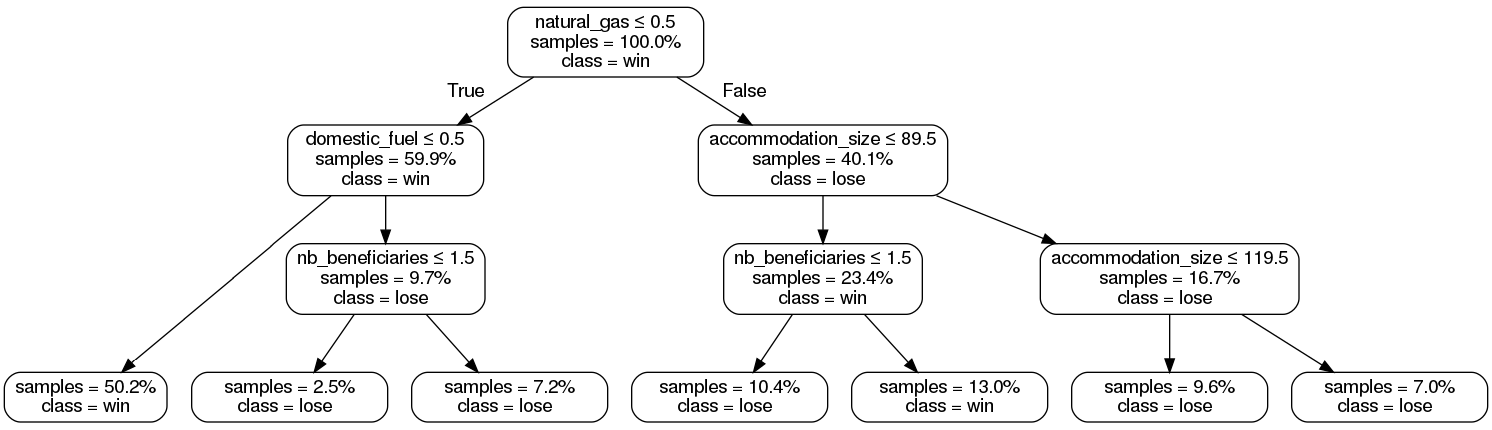
\includegraphics[width=\columnwidth]{Images/decision_tree_wo_values_wo_color.png}
% {\footnotesize \parbox[t]{15.5cm } {\linespread{1.2}\selectfont \textsc{Note:} This figure shows that 50.2\% of respondents who do not use natural gas or heating oil ($\leq 0.5$) as their heating source are predicted to win from the tax \& dividend. }} %
% \caption{Decision tree that classifies households into winners and losers.}
% \label{fig:tree}
% \end{figure}

% sss: wouldn't the figure "shows" be more appropriate than "reads"? %% RCP NOTE: Edited.

% dr2 : améliorer la note pour préciser ce à quoi correspond la courbe bleue (c'est déjà expliqué dans la phrase...). On peut ajouter "in the consumer survey, and the blue curve the probability that our net gains estimation correctly predicts the win/lose category. As shown..." => done
% dr2: changé l'axe du graphique -> je vois pas quel est le changeemnt => j'ai rajouté "correcty" dans "probability of correctly predicting gain" (il avait souligné cet oubli)

\begin{figure}[H]
\centering
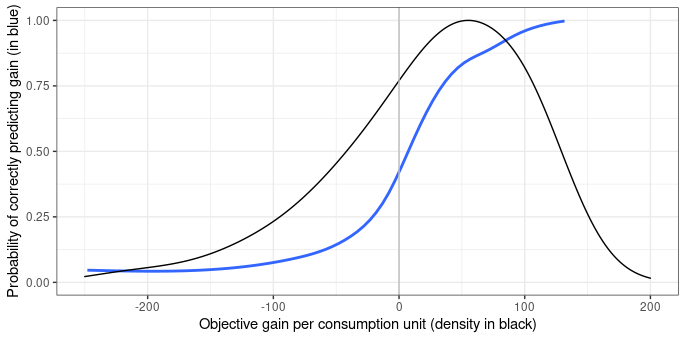
\includegraphics[width=0.85\columnwidth]{Images/prob_correct_prediction.png} \\[-1ex]
{\footnotesize \parbox[t]{15.5cm } {\linespread{1.2}\selectfont \textsc{Note:} The black curve corresponds to the density of households' objective net gains in the consumer survey, and the blue curve corresponds to the probability that our net gain estimation correctly predicts the win/lose category. As shown by the blue curve, households in the consumer survey who would gain 100\euros{} per c.u.---as directly computed from their energy bills---were predicted to be winners based on their energy characteristics in 96\% of cases. See the discussion in the main text, Section \vref{subsubsec:update_after_feedback}.}
\caption{Probability that our net gains estimation correctly predicts the win/lose category.\label{fig:proba_pred}}} %
\end{figure}

\vspace*{1.5cm}

\begin{figure}[ht!]
\centering
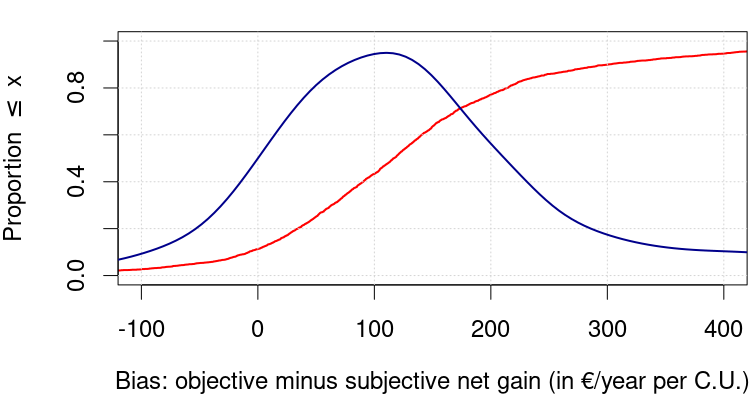
\includegraphics[width=.8\columnwidth]{Images/biais.png}
\parbox[t]{\columnwidth}{ %
\linespread{1.2}\selectfont \footnotesize{\textsc{Note:} The red curve indicates that for 11\% of the respondents, their objective gains are lower than their subjective ones; meanwhile, for 23\% of them, they are higher by at least 200\euros{}. The blue curve indicates that the most common bias is an underestimation of gains by approximately 100\euros{}. See the discussion in the main text, Section \vref{subsec:perc_si}. \caption{CDF (in red) and PDF (in blue) of the bias. \label{fig:bias}}}}
\end{figure}

\subsection{Distributional effects \label{subsec:app_distributive}}

\begin{figure}[H]
\begin{subfigure}{.5\textwidth}
\centering
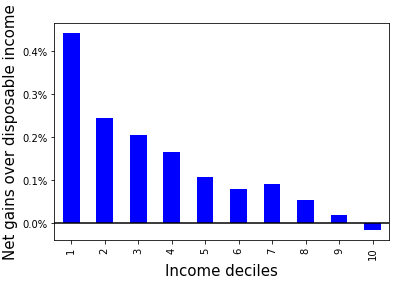
\includegraphics[scale=0.9]{Images/effort_rate_uc.png}
\end{subfigure}\hfill
\begin{subfigure}{.5\textwidth}
\centering
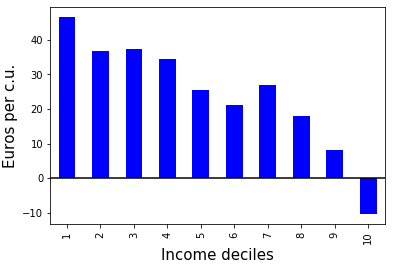
\includegraphics[scale=0.9]{Images/average_cost_decile.png}
\end{subfigure} \\[1ex]
{\footnotesize  \parbox[t]{15.5cm } {\linespread{1.2}\selectfont \textsc{Note:} Net gains are defined in equation (\ref{eq:formula_net_gain_app}). They correspond to the dividend minus the increase in expenditures ($\Delta E$), not in taxes ($\Delta T$). Although the latter would sum to zero overall because the reform is budget neutral, the former does not because fossil fuel expenditures adjust downwards following the increase in the carbon tax. See the discussion in the main text, Section \vref{subsec:beliefs_progressivity}.}
\caption{Average net gain of the carbon tax and dividend policy by income decile (computed using Insee data).\label{figure:effort_rate_uc}}
}
\end{figure}

\section{Beliefs and persistence\label{sec:app_perception}}

\subsection{Elasticities}

% dr2 : "perceived elasticity relates" -> "perceived elasticities relate"
% dr2 : "to perceive the policy" -> "to perceive the tax \& dividend policy"

% tr2 : Ici aussi on peut dire qu'on explique mieux les questions utilisées. edit!

% dr2 : ajout du paragraphe ci-dessous (précédemment en 3.2)
To see how perceived elasticities relate to the perception of effectiveness, we run two separate regressions where the dependent variable $E$ is equal to 0 if the respondent does not perceive the policy to be environmentally effective and 1 otherwise. In the first regression, we regress the perceived effectiveness on the perceived elasticity for housing; and in the second, we regress it on the perceived elasticity for transport energy. Table \ref{table:elasticities_effectiveness} below reports the results with and without control variables. They all consistently indicate that perceived elasticities are correlated with beliefs about the policy's effectiveness since for both sectors a respondent anticipating an elasticity of $-$1 is (on average) 6 p.p. more likely to perceive the tax \& dividend policy to be effective than one anticipating no elasticity. Although significant, the magnitude of the effect is modest, showing that the perceived ineffectiveness of tax instruments should not be attributed to small subjective elasticities.

\begin{table}[H] \centering 
  \caption{Effect of subjective elasticities on perceived environmental effectiveness.} 
  \label{table:elasticities_effectiveness} 
\makebox[\textwidth][c]{ \begin{tabular}{@{\extracolsep{5pt}}lcccc} 
\\[-2.1ex]\hline 
\hline \\[-1.8ex] 
\\[-4ex] & \multicolumn{4}{c}{Environmental effectiveness: not `No'} \\ 
\\[-2.1ex] & (1) & (2) & (3) & (4)\\ 
\hline \\[-1.8ex] 
 Price elasticity: Housing & $-$0.062 &  & $-$0.055 &  \\ 
  & (0.032) &  & (0.032) &  \\ 
  Price elasticity: Transport &  & $-$0.056 &  & $-$0.060 \\ 
  &  & (0.030) &  & (0.030) \\ 
 \hline \\[-2.3ex] 
Controls: Sociodemo, energy, &  &  & \checkmark   & \checkmark \\ 
\hspace{1.6cm} incomes, estimated gains &  &  &  & \\ 
Observations & 1,501 & 1,501 & 1,501 & 1,501 \\ 
R$^{2}$ & 0.003 & 0.002 & 0.089 & 0.090 \\ 
\hline 
\hline \\[-1.3ex] 

\end{tabular} 
}
{\footnotesize \parbox[t]{15.5cm } {\linespread{1.2}\selectfont \textsc{Note:} Environmental effectiveness refers to the belief that the policy would be effective at reducing pollution and fighting climate change. Price elasticities for housing and transport are elicited from respondents' expected reduction in energy consumption of French people following a given increase in energy prices. For more details, see the discussion in the main text, Section \vref{subsec:perception_ee}. The list of controls can be found in the Appendix \ref{set_controls}.}}
\end{table}


%dr2 : "Price elasticity: Transports" -> "Price elasticity: Transport" / ajout d'une virgule après "energy" dans les contrôles.
% dr2 : améliorer la note de cette table pour expliquer les régressions. Proposition : "Environmental effectiveness refers to the belief that the policy would be effective to reduce pollution and fight climate change. Price elasticities for housing and transport are elicited from people expected reduction in energy consumption of French people following a given increase in energy prices. For more details, see the discussion in the main text, Section \vref{subsec:perception_ee}. The list of controls can be found in Appendix \ref{set_controls}." => done en remplaçant "people expected" par "expected" -> donc on enlève people ? Tu l'as gardé actuellement. => ah oui >< bon j'ai remplacé par "respondents'" finalement -> ok

\vspace*{1.5cm}

\subsection{Self-interest \label{subsec:app_perception_si}}

\medskip

\begin{table}[H]
\caption[table]{Transition matrix after telling respondents they are expected to \textit{win} (75.8\%).}
{\label{table:transition_matrix_positive_feedback}}
\centering
\begin{tabular}{lccc}
\textit{Before $\setminus$ After} & \textbf{Winner} (25\%) & \textbf{Unaffected} (28\%) & \textbf{Loser} (47\%) \\
\hline
\textbf{Winner} (16\%) & 79\% & 13\% & 8\%\\
\textbf{Unaffected} (24\%) & 22\% & 63\% & 15\% \\
\textbf{Loser} (60\%) & 12\% & 18\% & 70\% \\ \\
\end{tabular}
{\footnotesize \\ $\quad$ \\[-3ex] \textsc{Note:} See the discussion in the main text, Section \vref{subsubsec:update_after_feedback}.}
\end{table}

\vspace{1cm}

\begin{table}[H]
\caption[table]{Transition matrix after telling respondents they are expected to \textit{lose} (24.2\%).}
{\label{table:transition_matrix_negative_feedback}}
\centering
\begin{tabular}{lccc}
\textit{Before $\setminus$ After} & \textbf{Winner} (3\%) & \textbf{Unaffected} (12\%) & \textbf{Loser} (86\%) \\
\hline
\textbf{Winner} (7\%) & 16\% & 3\% & 81\% \\
\textbf{Unaffected} (15\%) & 5\% & 50\% & 46\% \\
\textbf{Loser} (78\%) & 1\% & 5\% & 94\% \\ \\
\end{tabular}
{\footnotesize \\ $\quad$ \\[-3ex] \textsc{Note:} See the discussion in the main text, Section \vref{subsubsec:update_after_feedback}.}
\end{table}

\vspace{1.5cm}

\begin{table}[H] \centering 
  \caption{Share with new beliefs aligned with feedback, among those with a large gain or loss $(|\widehat{\gamma}| > 110)$.}
  \label{table:confidence_intervals_beliefs_feedback_biased} 
\begin{tabular}{@{\extracolsep{5pt}}lcc} 
\\[-1.8ex]\hline 
\hline \\[-1.8ex] 
 & \multicolumn{2}{c}{\textit{Aligned with feedback: $G^F = \widehat{\Gamma}$}} \\ 
\cline{2-3} 
\\[-1.8ex] & win ($\widehat{\Gamma} = 1$) & lose ($\widehat{\Gamma} = 0$) \\ \vspace*{0.5cm} & (81.6\%)  & (18.4\%) \\ \hline \\[-1.8ex] 
 Initial belief winner ($g > 0$) & 77.6\% & 78.4\% \\ 
 (19.4\%) & {\small $\left[68.5\% ; 84.7\%\right]$} & {\small $\left[43.2\% ; 94.5\%\right]$} \\ 
 Initial belief unaffected ($g = 0$) & 20.7\% & 32.7\% \\ 
 (28.2\%) & {\small $\left[14.8\% ; 28.1\%\right]$} & {\small $\left[14.7\% ; 57.7\%\right]$} \\ 
 Initial belief loser ($g < 0$) & 10.8\% & 92.2\% \\ 
 (52.3\%) & {\small $\left[7.3\% ; 15.8\%\right]$} & {\small $\left[84.5\% ; 96.3\%\right]$} \\ 
 Initial belief affected ($g \neq 0$) & 32.7\% & 91.1\% \\ 
 (70.8\%) & {\small $\left[27.7\% ; 38.1\%\right]$} & {\small $\left[83.5\% ; 95.4\%\right]$} \\ 
  & & \\[-1.8ex] \hline \\[-1.8ex]
 All & 28.9\% & 83.0\% \\ 
 (100\%) & {\small $\left[24.8\% ; 33.3\%\right]$} & {\small $\left[74.8\% ; 88.9\%\right]$} \\ 
 & & \\
 [-1.8ex]\hline 
\hline \\[-1.0ex]
\end{tabular}
{\footnotesize \parbox[t]{12cm } {\linespread{1.2}\selectfont\textsc{Note:} The 95\% confidence intervals for binomial probabilities are given in brackets. The table reads as follows: among those who initially think that they would win ($g^0 > 0$) but are told they are expected to lose ($\hat{\Gamma} = 0$), 78.4\% agree that they would lose ($G^F = 0$). Compared to Table 4.1, this table focuses on the subsample of 546 respondents with a large gain or loss ($|\widehat{\gamma}| > 110$)) who received feedback. See the discussion in the main text, Section \vref{subsubsec:update_after_feedback}.}}
\end{table}

% dr2 : provide sample size in the Note of the table above ? => ok -> "the subsample of people with a large gain or loss ($|\widehat{\gamma}| > 110$))." -> "the subsample of 546 respondents with a large gain or loss ($|\widehat{\gamma}| > 110$)) who received a feedback."

% dr2 : on écrit parfois "subsample" et parfois "sub-sample", il faudrait uniformiser (je n'ai pas de préférence les deux sont corrects). => done sans tiret

\clearpage

\subsection{Environmental effectiveness \label{subsec:app_perception_ee}}

%dr2 : "Effect of primings" -> "Effect of information interventions"

\begin{table}[!htbp] \centering 
  \caption{Effect of information interventions on beliefs about environmental effectiveness} 
  \label{tab:update_ee} 
\makebox[\textwidth][c]{ \begin{tabular}{@{\extracolsep{5pt}}lcccc} 
\\[-4ex]\hline 
\hline \\[-2.3ex] 
 & \multicolumn{4}{c}{Environmental effectiveness} \\ 
\cline{2-5} 
\\[-2.3ex] & \multicolumn{3}{c}{not ``No''} & ``Yes'' \\ 
\\[-2.3ex] & \multicolumn{2}{c}{\textit{OLS}} & \textit{logit} & \textit{OLS} \\ 
 & (1) & (2) & (3) & (4) \\ 
\hline \\[-1.8ex] 
 Info on Environmental Effectiveness ($Z_{E}$) & 0.043 & 0.063 & 0.052 & 0.059 \\ 
  & (0.017) & (0.018) & (0.018) & (0.014) \\ 
  Info on Climate Change ($Z_{CC}$) & 0.044 & 0.041 & 0.043 & 0.029 \\ 
  & (0.024) & (0.024) & (0.024) & (0.018) \\ 
  Info on Particulate Matter ($Z_{PM}$) & 0.039 & 0.029 & 0.037 & 0.017 \\ 
  & (0.024) & (0.024) & (0.024) & (0.019) \\ 
  $Z_{CC} \times Z_{PM}$ & $-$0.040 & $-$0.033 & $-$0.042 & $-$0.005 \\ 
  & (0.035) & (0.034) & (0.033) & (0.027) \\ 
 \hline \\[-2.3ex] 
Controls: Sociodemo  &  & \checkmark  & \checkmark  & \checkmark  \\ 
Observations & 3,002 & 3,002 & 3,002 & 3,002 \\ 
R$^{2}$ & 0.003 & 0.047 &  & 0.075 \\ 
\hline 
\hline \\[-1ex] 

\end{tabular} 
}
 {\footnotesize \textsc{Note:} See the discussion in the main text, Section \vref{subsec:update_ee}.}
 \end{table}

\vspace{-0.3cm}

\clearpage
\subsection{Progressivity \label{subsec:app-prog}}

\begin{table}[!htbp] \centering 
  \caption{Effect of information on perceived progressivity} 
  \label{tab:prog} 
\makebox[\textwidth][c]{ \begin{tabular}{@{\extracolsep{5pt}}lccc} 
\\[-4ex]\hline 
\hline \\[-4ex] 
\\[-1.8ex] & \multicolumn{3}{c}{Progressivity: not ``No'' ($P$)} \\ 
\\[-1.8ex] & (1) & (2) & (3)\\ 
\hline \\[-1.8ex] 
 Constant & 0.419 & 0.435 & 0.052 \\ 
  & (0.022) & (0.033) & (0.319) \\ 
  Information on progressivity ($Z_P$) & $-$0.021 & 0.050 & 0.051 \\ 
  & (0.027) & (0.040) & (0.041) \\ 
  Large bias $(\left|\widehat{\gamma}-g\right|>110)$ &  & $-$0.028 & $-$0.040 \\ 
  &  & (0.045) & (0.045) \\ 
  Interaction $Z_P \times (\left|\widehat{\gamma}-g\right|>110)$ &  & $-$0.130 & $-$0.117 \\ 
  &  & (0.055) & (0.055) \\ 
 \hline \\[-1.8ex] 
Controls: Sociodemo, politics  &  &  & \checkmark  \\ 
Observations & 1,444 & 1,444 & 1,444 \\ 
R$^{2}$ & 0.0004 & 0.018 & 0.094 \\ 
\hline 
\hline \\[-1ex] 
  
\end{tabular} 
 }
 {\footnotesize \parbox[t]{12cm } {\linespread{1.2}\selectfont \textsc{Note:} A large bias is defined as a difference between the subjective (g) and objectively estimated ($\hat{\gamma})$ net gain larger than 110\euros{}/year per c.u. See the discussion in the main text, Section \vref{subsec:persistence-prog}.}}
 \end{table}





\clearpage

% \section{Estimation of acceptation motives \label{sec:app_motives}}

% \subsection{Two-stage least squares: first-stage results\label{subsec:app_motives_1st_stage}}

% \begin{table}[!htbp] \centering 
%   \caption{First-stage regressions results for self-interest} 
%   \label{first_stage_private_benefits} 
% \makebox[\textwidth][c]{ \begin{tabular}{@{\extracolsep{5pt}}lccc} 
% \\[-1.8ex]\hline 
% \hline \\[-2.1ex] 
%  & \multicolumn{3}{c}{Believes does not lose} \\ 
% \cline{2-4} 
% \\[-1.8ex] & \multicolumn{2}{c}{Targeted Dividend ($G^T$)} & After feedback ($G^F$) \\ 
%  & (1) & (2) & (4) \\ 
% \hline \\[-2.1ex] 
%  Transfer to respondent ($T_1$) & 0.199 & 0.224 &  \\ 
%   & (0.034) & (0.030) &  \\ 
%   Transfer to spouse ($T_2$) & 0.172 & 0.156 &  \\ 
%   & (0.042) & (0.039) &  \\ 
%   $T_1 \times T_2$ & $-$0.145 & $-$0.158 &  \\ 
%   & (0.045) & (0.037) &  \\ 
%   Predicted winner ($\widehat{\Gamma}$) &  &  & 0.269 \\ 
%   &  &  & (0.058) \\ 
%   Initial tax Acceptance ($A^0$) & 0.123 & 0.154 & 0.306 \\ 
%   & (0.041) & (0.033) & (0.066) \\ 
%  \hline \\[-2.1ex] 
% Controls: Incomes (piecewise continuous) &  \checkmark &  \checkmark & \checkmark \\ 
% \quad estimated gains, sociodemo, other motives  &  &  &  \\ 
% Controls: Policy assigned &  \checkmark &  \checkmark &   \\ 
% Subsample & [p10; p60] &  & $\left| \widehat{\gamma}\right|<50$ \\ 
% Effective F-statistic & 15.6 & 23.8 & 21.3 \\ 
% Observations & 1,969 & 3,002 & 757 \\ 
% R$^{2}$ & 0.221 & 0.196 & 0.301 \\ 
% \hline 
% \hline \\[-1.8ex] 
% \end{tabular} 
% } {\footnotesize \parbox[t]{\textwidth}{\linespread{1.2}\selectfont \textsc{Note:} In (1,2), the random eligibility for the dividend (conditional on income) is used as a source of exogenous variation in the belief. In (4), the discontinuity in the win/lose feedback when the net gain switches from negative to positive is used. Column numbers correspond to second-stage results, Table \vref{results_private_benefits}. }} \end{table}

% %dr2 : "Simulated winner" -> "Predicted winner".

% \begin{table}[!htbp] \centering 
%   \caption{First-stage regressions results for environmental effectiveness} 
%   \label{first_stage_environmental_effectiveness} 
% \makebox[\textwidth][c]{ \begin{tabular}{@{\extracolsep{5pt}}lcc} 
% \\[-1.8ex]\hline 
% \hline \\[-2.1ex] 
%  & \multicolumn{2}{c}{Environmental effectiveness} \\ 
% \cline{2-3} 
% \\[-1.8ex] & ``Yes'' & not ``No'' \\ 
%  & (1; 3) & (A4) \\ 
% \hline \\[-2.1ex] 
%  Info on Environmental Effectiveness ($Z_{E}$) & 0.059 & 0.062 \\ 
%   & (0.014) & (0.017) \\ 
%   Info on Climate Change ($Z_{CC}$) & 0.028 & 0.030 \\ 
%   & (0.013) & (0.017) \\ 
%  \hline \\[-2.1ex] 
% Controls: Socio-demo, other motives, & \checkmark  & \checkmark  \\ 
% \quad incomes, estimated gains   & &  \\ 
% Effective F-statistic & 11.2 & 6.0 \\ 
% Observations & 3,002 & 3,002 \\ 
% R$^{2}$ & 0.123 & 0.121 \\ 
% \hline 
% \hline \\[-1.8ex] 
% \end{tabular} 
% } {\footnotesize  \parbox[t]{.8\textwidth}{\linespread{1.2}\selectfont \textsc{Note:} In column names, (A4) refers to columns with alternative second stages in Table \ref{tab:eea}. The information randomly displayed about climate change ($Z_{CC}$) and the effectiveness of carbon taxation ($Z_{E}$) is used as sources of exogenous variation in the belief. We chose the set of instruments that maximizes the effective F-statistics. The Sargan test does not reject the validity of our overidentification restrictions (p-value of 0.93). See the discussion in the main text, Section \vref{subsec:motive_ee}.}} \end{table}

% %dr2 : suppression de "Our specification is well founded because" avant "The Sargan test".

% \clearpage
% dr2 supprimer les tables de l'appendix, renommer la section: Additional specifications
% dr2 renommer cette section: "Additional specifications for the estimation of acceptation motives" (remplace "Additional specifications")
\section{Additional specifications for the estimation of acceptation motives \label{subsec:app_motives_other}}

\begin{table}[!htbp] \centering 
  \caption{Effect of self-interest on acceptance: second stages of alternative specifications} 
  \label{tab:alternative_si} 
\makebox[\textwidth][c]{ \begin{tabular}{@{\extracolsep{5pt}}lcccccc} 
\\[-1.8ex]\hline 
\hline \\[-1.8ex] 
 & \multicolumn{3}{c}{Targeted Dividend ($A^T$)} & \multicolumn{3}{c}{After Feedback ($A^F$)} \\ 
\cline{2-7} 
\\[-1.8ex] & Acceptance & \multicolumn{2}{c}{Approval} & Acceptance & \multicolumn{2}{c}{Approval} \\ 
\\[-1.8ex] & (1) & (2) & (3) & (4) & (5) & (6)\\ 
\hline \\[-1.8ex] 
 Believes wins & 0.574 & 0.357 &  & 1.131 & 0.609 &  \\ 
  & (0.136) & (0.117) &  & (0.298) & (0.233) &  \\ 
  Believes does not lose &  &  & 0.343 &  &  & 0.347 \\ 
  &  &  & (0.113) &  &  & (0.133) \\ 
 \hline \\[-1.8ex] 
Controls: Incomes (piecewise continuous) & \checkmark  & \checkmark   & \checkmark  & \checkmark & \checkmark  & \checkmark \\ 
\quad estimated gains, sociodemo, other motives  &  &  &  &  &  &  \\ 
Controls: Policy assigned & \checkmark  & \checkmark  & \checkmark   &  &  &  \\ 
Subsample: [p10; p60] ($A^T$) or $\left| \widehat{\gamma}\right|<50$ ($A^F$) & \checkmark  & \checkmark   & \checkmark  & \checkmark & \checkmark  & \checkmark \\ 
Effective F-Statistic & 21.3 & 21.3 & 15.6 & 11.4 & 11.4 & 21.3 \\ 
Observations & 1,969 & 1,969 & 1,969 & 757 & 757 & 757 \\ 
R$^{2}$ & 0.321 & 0.217 & 0.217 & 0.541 & 0.518 & 0.518 \\ 
\hline 
\hline \\[-1.8ex] 
\end{tabular} 
} {\footnotesize \parbox[t]{\textwidth}{\linespread{1.2}\selectfont \textsc{Note:} See the results of the main specifications, Table \vref{results_private_benefits}. As in the latter table, the source of exogenous variation in the belief used in first stages for the targeted dividend is the random assignment of the income threshold, which determines eligibility for the dividend. The first stage for the non-targeted dividend instead exploits the discontinuity in the win/lose feedback when the net gain switches from negative to positive.} }.\end{table}


% sr2 (voix passive) : "the source of exogenous variation in the belief used in first stages" -> "the source of exogenous variation in the belief we use in first stages" => je laisserais ici

% sss there are several incomes (respondent + spouse), so maybe plural is justified %% RCP NOTE: "Incomes" sounds awkward to a native English speaker in this context. -> je lui fais confiance, ça doit être les revenus en règle général qui est bien traduit par "income".
\begin{table}[!htbp] \centering 
  \caption{Effect of self-interest on acceptance: the role of income \label{tab:alternative_sio}} 
 
\makebox[\textwidth][c]{ \begin{tabular}{@{\extracolsep{5pt}}lccccc} 
\\[-1.8ex]\hline 
\hline \\[-2.1ex] 
\\[-1.8ex] & \multicolumn{5}{c}{Acceptance of Tax \& Targeted Dividend ($A^T$)} \\ 
\\[-1.8ex] & (1) & (2) & (3) & (4) & (5)\\ 
\hline \\[-1.8ex] 
 Believes does not lose ($G^T$) & 0.773 & 0.556 & 0.549 & 0.535 & 0.502 \\ 
  & (0.222) & (0.133) & (0.133) & (0.133) & (0.130) \\ 
  Income above 35th percentile ($\un_{I > p35}$) & 0.343 &  &  &  &  \\ 
  & (0.508) &  &  &  &  \\ 
  $G^T \times \un_{I > p35}$ & $-$0.392 &  &  &  &  \\ 
  & (0.311) &  &  &  &  \\ 
  Initial policy Acceptance ($A^0$) & 0.387 & 0.353 & 0.354 & 0.356 & 0.359 \\ 
  & (0.058) & (0.041) & (0.041) & (0.041) & (0.040) \\ 
 \hline \\[-1.8ex] 
Percentile with additional income slope change &  & 30 & 40 & 50 & 60 \\ 
Controls: Incomes (piecewise continuous) & \checkmark  & \checkmark   & \checkmark  & \checkmark & \checkmark  \\ 
\quad estimated gains, sociodemo, other motives  &  &  &  &  &  \\ 
Subsample: [p10; p60]; Controls: Policy assigned & \checkmark   & \checkmark  & \checkmark & \checkmark  & \checkmark \\ 
Effective F-statistic & 5.5 & 15.3 & 15.2 & 15.2 & 16.1 \\ 
Observations & 1,969 & 1,969 & 1,969 & 1,969 & 1,969 \\ 
R$^{2}$ & 0.571 & 0.321 & 0.321 & 0.321 & 0.321 \\ 
\hline 
\hline \\[-1.8ex] 
\end{tabular} 
} {\footnotesize \parbox[t]{\textwidth}{\linespread{1.2}\selectfont \textsc{Note:} See the results of the main specifications, Table \vref{results_private_benefits}. The source of the exogenous variation in the belief used in the first stage is the random assignment of the income threshold, which determines eligibility for the dividend.} }\end{table}
% dr2 : "Initial tax Acceptance ($A^0$)" -> "Initial policy Acceptance ($A^0$)"

% sr2 (voix passive) : "used in the first stage" -> "we use in the first stage" => je laisserais ici

\begin{table}[!htbp] \centering 
  \caption{Effect of believing in environmental effectiveness on support: second stages of alternative specifications} 
  \label{tab:eea} 
\makebox[\textwidth][c]{ \begin{tabular}{@{\extracolsep{5pt}}lcccc} 
\\[-1.8ex]\hline 
\hline \\[-1.8ex] 
 & \multicolumn{4}{c}{Initial Tax \& Dividend} \\ 
\cline{2-5} 
\\[-1.8ex] & \multicolumn{4}{c}{Approval ($\dot{A^0}$)} \\ 
 & $LIML$ & $OLS$ & $IV$ & $OLS$ \\ 
\\[-1.8ex] & (A1) & (A2) & (A3) & (A4)\\ 
\hline \\[-1.8ex] 
 Environmental effectiveness: ``Yes'' & 0.643 & 0.367 &  &  \\ 
  & (0.320) & (0.020) &  &  \\ 
  Environmental effectiveness: not ``No'' &  &  & 0.479 & 0.413 \\ 
  &  &  & (0.230) & (0.015) \\ 
 \hline \\[-1.8ex] 
Instruments: info E.E. \& C.C.  & \checkmark  &  & \checkmark  &  \\ 
Controls: Sociodemo, other motives  & \checkmark   & \checkmark  & \checkmark  & \checkmark  \\ 
Effective F-statistic &  &  & 6.0 &  \\ 
Observations & 3,002 & 3,002 & 3,002 & 3,002 \\ 
R$^{2}$ & 0.295 & 0.295 & 0.218 & 0.379 \\ 
\hline 
\hline \\[-1.8ex] 
\end{tabular} 
} {\footnotesize \parbox[t]{\textwidth}{\linespread{1.2}\selectfont \textsc{Note:} Standard errors are reported in parentheses. The list of controls can be found in the Appendix \ref{set_controls} and the main results in Table \vref{tab:ee}. As in the latter table, the dependent variable corresponds to either initial approval (answer ``Yes'' to support for the policy) or acceptance (answer not ``No''). The first stage exploits the information randomly displayed about climate change (C.C.) and the effectiveness of carbon taxation (E.E.) as exogenous instruments.}}\end{table}

\clearpage

\section{Control variables}\label{set_controls}

\textbf{Sociodemo:} \textit{respondent's income, household's income, sex, age \textnormal{(5 categories)}, employment status \textnormal{(9 categories)}, socioprofessional category \textnormal{(8 categories)}, region of France \textnormal{(10 categories)}, size of town \textnormal{(5 categories)}, diploma \textnormal{4 categories}, household size, number of people above 14, number of adults, number of c.u., income per c.u., smokes, favored media for news \textnormal{(5 categories)}.}

\vspace{0.5cm}

\noindent
\textbf{Politics:} \textit{extreme left, left, center, right, extreme right, interest in politics \textnormal{(3 categories)}, conservative, liberal, humanist, patriot, environmentalist, apolitical.}

\vspace{0.5cm}

\noindent
\textbf{Political leaning:} \textit{extreme left, left, center, right, extreme right, indeterminate.}

\vspace{0.5cm}

\noindent
\textbf{Energy:} \textit{heating mode \textnormal{(collective vs. individual)}, heating energy \textnormal{(7 categories)}, annual distance travelled, fuel economy, diesel \textnormal{(binary)}, gasoline \textnormal{(binary)}, number of vehicles.}

\vspace{0.5cm}

\noindent
\textbf{Incomes:} \textit{income of respondent, income of the second adult, income of respondent squared, income of the second adult squared, dummy for absence of second adult.}

\vspace{0.5cm}

\noindent
\textbf{Incomes (piecewise continuous):} \textit{income percentile of respondent ($I_1$), income percentile of the second adult ($I_2$), dummy for absence of second adult, $\min\left(I_1-20,\:0\right)$, $\min\left(I_1-70,\:0\right)$, $\min\left(I_2-20,\:0\right)$, $\min\left(I_2-70,\:0\right)$.}

\vspace{0.5cm}

\noindent
\textbf{Estimated gains:} \textit{simulated net gain, squared simulated gain.}

\clearpage

\begin{center}
    {\huge \textbf{Online Appendix}}
\end{center}

\section{Questionnaire (\emph{For online publication})} \label{sec:questionnaire} 

%dr2 : "+5°C -> +5°C", pareil pour +8 et +2.
%dr2 : "Brevet des collÚges" -> "Brevet des collèges".

% dr2 : "Priming" -> "Information intervention". Au pluriel ? => nope
%dr2 : "No priming" -> "No information"

\paragraph{Information intervention}
\begin{enumerate}[leftmargin=*]
\item {[}No information{]} Welcome to this survey. \\
It was conceived by two social science researchers. It lasts about
15-20 minutes.
\item {[}Info PM{]} Welcome to this survey. \\
It was conceived by two social science researchers. It lasts about
15-20 minutes.\\
\\
Before starting, please read carefully the information below on particulate
matter pollution: 
\end{enumerate}
\begin{itemize}
\item particulate matter is responsible for 48,000 deaths in France each
year; 
\item particulate matter reduces the life expectancy of French people by
9 months; 
\item reducing fuel consumption would reduce the health problems associated
with particulate matter. \\
\\
Source: \href{https://www.santepubliquefrance.fr/content/download/189662/2330878}{France Public Health Report (2016)}
\end{itemize}
\begin{enumerate}[resume,leftmargin=*]
\item {[}Info CC{]} Welcome to this survey. \\
It was conceived by two social science researchers. It lasts about
15-20 minutes.\\
\\
Please read carefully the information below on climate change. \\
\end{enumerate}
\begin{itemize}
\item Climate change is already responsible for 150,000 deaths annually.
\item If greenhouse gas emissions continue on their current trend, the average
global temperature increase will be +5°C in 2100 and +8°C in 2250. 
\item A rapid transition to renewable energies is technically possible and
would contain global warming at +2°C. 
\end{itemize}
According to scientists, in the absence of ambitious measures, the following would occur: 
\begin{itemize}
\item a large proportion of species will face an increased risk of extinction,
\item natural disasters will intensify (hurricanes, heat waves, droughts,
floods, forest fires, etc.); 
\item by 2100, 270 million more people would be flooded each year due to
sea-level rise; 
\item violent conflicts and migration flows can be expected to increase. 
\end{itemize}
Sources: \href{http://www.pnas.org/content/106/49/20670}{Burke et al (2009)},
\href{http://www.pnas.org/content/pnas/early/2014/01/29/1222469111.full.pdf}{Hinkel et al (2014)},
\href{http://www.ipcc.ch/report/ar5/syr/}{IPCC Report (2014)}, \href{https://link.springer.com/article/10.1007/s10584-011-0156-z}{Meinshausen et al (2011)},
\href{https://www.nature.com/articles/nature04188}{Patz et al (2005)}

\paragraph{Sociodemographics}
\begin{enumerate}[resume,leftmargin=*]
\item What is your postal code? 
\item What is your gender (in the sense of civil status)? \emph{}\\
\emph{Female; Male }
\item What is your age group? \emph{}\\
\emph{18 to 24 years old; 25 to 34 years old; 35 to 49 years old;
50 to 64 years old; 65 years old or more} 
\item What is your employment status? \emph{}\\
\emph{Permanent; Temporary contract; Unemployed; Student; Retired;
Other active; Inactive}
\item What is your socioprofessional category? (Remember that the unemployed
are active workers). \emph{}\\
\emph{Farmer; Craftsperson, merchant; Independent; Executive; Intermediate
occupation; Employee; Worker; Retired; Other Inactive} 
\item What is your highest degree? \emph{}\\
\emph{No diploma; Brevet des collèges; CAP or BEP {[}secondary{]};
Baccalaureate; Bac +2 (BTS, DUT, DEUG, schools of health and social
training, etc.); Bac +3 (licence...) {[}bachelor's{]}; Bac +5 or more (master's,
engineering or business school, doctorate, medicine, master, DEA,
DESS, etc.)}
\item How many people live in your household? Your household includes the following: you, your
family members who live with you, and your dependents. 
\item What is your net \textbf{\underline{monthly}} income (in euros)? \textbf{\underline{All
income}} (before withholding tax) is included here: salaries, pensions,
allowances, APL {[}housing allowance{]}, land income, etc. 
\item What is the net \textbf{\underline{monthly}} income (in euros) \textbf{\underline{of
your household}}? \textbf{\underline{All income}} (before withheld
taxes) is included here: salaries, pensions, allowances, APL {[}housing
allowance{]}, land income, etc. 
\item In your household, how many people are 14 years old or older (\textbf{\underline{including
yourself}})? 
\item In your household, how many people are over the age of majority
%Editor: Please consider clarifying “majority” in the above line. Perhaps “the majority”, “14”, “18”, or “adulthood” is more precise here.
(\textbf{\underline{including
yourself}})? 
\end{enumerate}

\paragraph{Energy characteristics}
\begin{enumerate}[resume,leftmargin=*]
\item What is the surface area of your home? (in m\texttwosuperior )
\item What is the heating system in your home? \emph{}\\
\emph{Individual heating; Collective heating; PNR (Don't know, don't
say)}
\item What is the main heating energy source in your home? \emph{}\\
\emph{Electricity Town gas; Butane, propane, tank gas; Heating oil;
Wood, solar, geothermal, aerothermal (heat pump); Other; PNR (Don't
know, don't say)}
\item How many motor vehicles does your household have? \emph{}\\
\emph{None; One; Two or more} 
\item {[}Without a vehicle{]} How many kilometers have you driven in the
last 12 months? 
\item {[}One vehicle{]} What type of fuel do you use for this vehicle? \emph{}\\
\emph{Electric or hybrid; Diesel; Gasoline; Other} 
\item {[}One vehicle{]} What is the average fuel economy of your vehicle?
(in Liters per 100 km)
\item {[}One vehicle{]} How many kilometers have you driven your vehicle
in the last 12 months?
\item {[}At least two vehicles{]} What type of fuel do you use for your
main vehicle?\\
\emph{Electric or hybrid; Diesel; Gasoline; Other} 
\item {[}At least two vehicles{]} What type of fuel do you use for your
second vehicle?\\
\emph{Electric or hybrid; Diesel; Gasoline; Other} 
\item {[}At least two vehicles{]} What is the average fuel economy of all
your vehicles? (in Liters per 100 km) 
\item {[}At least two vehicles{]} How many kilometers have you driven in
all your vehicles in the last 12 months? 
\end{enumerate}

%dr2 : "uc" > "c.u."

\paragraph{Partial reforms {[}transport / housing{]}}
\begin{enumerate}[resume,leftmargin=*]
\item Do you think that an increase in the VAT would result in a loss of more
purchasing power for your household than for the average French household?
\emph{}\\
\emph{Yes, much more; Yes, a little more; As much as the average;
No, a little less; No, a lot less; or PNR (Don't know, don't say)} 
\item Do you think that an increase in {[}fuel taxes / taxes on gas and
heating oil{]} would cause your household to lose more purchasing
power than an average French household? \emph{}\\
\emph{Yes, much more; Yes, a little more; As much as the average;
No, a little less; No, a lot less; or PNR (Don't know, don't say)}
\item The government is studying a fuel tax increase whose revenues would
be redistributed to all households, regardless of their income. This
would imply the following: 
\end{enumerate}
\begin{itemize}
\item {[}an increase in the price of gasoline by 11 cents per liter and
diesel by 13 cents per liter / a 13\% increase in the price of gas,
and a 15\% increase in the price of heating oil{]}; and 
\item an annual payment of {[}60 / 50{]}\euros{} to each adult, or {[}120 / 100{]}\euros{}
per year for a couple. \\
\\
\textbf{In terms of purchasing power, would your household be a winner
or a loser with such a measure?} \emph{}\\
\emph{Winner; Unaffected; Loser} 
\end{itemize}
\begin{enumerate}[resume,leftmargin=*]
\item {[}\emph{Winner} selected{]} \textbf{According to you, your household's
purchasing power would increase:} \emph{}\\
\emph{From 0 to {[}10$\cdot$c.u.{]} \euros{} per year; From {[}10$\cdot$c.u.{]}
to {[}20$\cdot$c.u.{]} \euros{} per year; From {[}20$\cdot$c.u.{]} to {[}30$\cdot$c.u.{]}
\euros{} per year; From {[}30$\cdot$c.u.{]} to {[}40$\cdot$c.u.{]} \euros{} per year;
More than {[}40$\cdot$c.u.{]} \euros{} per year}
\item {[}\emph{Loser} selected{]} \textbf{According to you, the purchasing
power of your household would decrease by how much:} \emph{}\\
\emph{From 0 to {[}15$\cdot$c.u.{]} \euros{} per year; From {[}15$\cdot$c.u.{]}
to {[}40$\cdot$c.u.{]} \euros{} per year; From {[}40$\cdot$c.u.{]} to {[}70$\cdot$c.u.{]}
\euros{} per year; From {[}70$\cdot$c.u.{]} to {[}110$\cdot$c.u.{]} \euros{} per year;
From {[}110$\cdot$c.u.{]} to {[}160$\cdot$c.u.{]} \euros{} per year; More
than {[}160$\cdot$c.u.{]} \euro{} per year}
\item If fuel prices increased by 50 cents per liter, by how much would
\textbf{\underline{your household}} reduce its fuel consumption? \emph{}\\
\emph{0\% -} {[}\emph{I already consume almost none }/\emph{ I am
already not consuming}{]}\emph{; 0\% - }{[}\emph{I am constrained
on all my trips} / \emph{I will not reduce it}{]}\emph{; From 0\%
to 10\%; From 10\% to 20\%; From 20\% to 30\%; More than 30\% - }{[}\emph{I
would change my travel habits significantly }/ \emph{I would change
my consumption significantly}{]}
\item In your opinion, if {[}fuel prices increased by 50 cents per liter
/ gas and heating oil prices increased by 30\%{]}, by how much would
\textbf{\underline{French people}} reduce their consumption on average?
\emph{}\\
\emph{From 0\% to 3\%; From 3\% to 10\%; From 3\% to 10\%; From 10\%
to 20\%; From 20\% to 30\%; More than 30\%} 
\item Do you think that an increase in taxes on gas and heating oil would cause your household to lose more purchasing power than the average French household?\\
\emph{Yes, a lot more; Yes, a little more; As much as average; No, a little less; No, a lot less; PNR (Don't know, don't say)} %
\end{enumerate}

\paragraph{Tax \& dividend: initial}
\begin{enumerate}[resume,leftmargin=*]
\item \label{questionnaire:TD}The government is studying an increase in the carbon tax whose revenues
would be redistributed to all households, regardless of their income.
This would imply the following: 
\end{enumerate}
\begin{itemize}
\item an increase in the price of gasoline by 11 cents per liter and diesel
by 13 cents per liter; 
\item an increase of 13\% in the price of gas, and 15\% in the price of
heating oil; and
\item an annual payment of 110\euros{} to each adult, or 220\euros{} per year for a couple.
\\
\\
\textbf{In terms of purchasing power, would your household win or
loser with such a measure? }\emph{}\\
\emph{Win; Be unaffected; Lose}
\end{itemize}
\begin{enumerate}[resume,leftmargin=*]
\item {[}\emph{Winner} selected{]} \textbf{According to you, your household's
purchasing power would increase by how much:} \emph{}\\
\emph{From 0 to {[}20$\cdot$c.u.{]} \euros{} per year; From {[}20$\cdot$c.u.{]}
to {[}40$\cdot$c.u.{]} \euros{} per year; From {[}40$\cdot$c.u.{]} to {[}60$\cdot$c.u.{]}
\euros{} per year; From {[}60$\cdot$c.u.{]} to {[}80$\cdot$c.u.{]} \euros{} per year;
More than {[}80$\cdot$c.u.{]} \euros{} per year}
\item {[}\emph{Loser} selected{]} \textbf{According to you, the purchasing
power of your household would decrease by how much:} \emph{}\\
\emph{From 0 to {[}30$\cdot$c.u.{]} \euros{} per year; From {[}30$\cdot$c.u.{]}
to {[}70$\cdot$c.u.{]} \euros{} per year; From {[}70$\cdot$c.u.{]} to {[}120$\cdot$c.u.{]}
\euros{} per year; From {[}120$\cdot$c.u.{]} to {[}190$\cdot$c.u.{]} \euros{} per
year; From {[}190$\cdot$c.u.{]} to {[}280$\cdot$c.u.{]} \euros{} per year;
More than {[}280$\cdot$c.u.{]} \euros{} per year} 
\item {[} {[}empty{]} / Scientists agree that a carbon tax would be effective
in reducing pollution.{]} Do you think that such a measure would reduce
pollution and fight climate change? \emph{}\\ 
\emph{Yes; No; PNR (Don't know, don't say)}
\item In your opinion, which categories would lose {[} {[}blank{]} / purchasing
power{]} with such a measure? (Several answers possible) \emph{}\\
\emph{No one; The poorest; The middle classes; The richest; All French
people; Rural or peri-urban people; Some French people, but not a
particular income category; PNR (Don't know, don't say)} 
\item In your opinion, what categories would gain purchasing power with
such a measure? (Several answers possible) \emph{}\\
\emph{No one; The poorest; The middle classes; The richest; All French
people; Urban dwellers; Some French people, but not a particular income
category; PNR (Don't know, don't say)} 
\item Would you approve of such a measure?
\emph{}\\
\emph{Yes; No; PNR (Don't know, don't say)} 
\end{enumerate}

\paragraph{Tax \& dividend: after information}
\begin{enumerate}[resume,leftmargin=*]
\item {[}Feedback{]} We always consider the same measure. As a reminder,
it would imply the following: 
\end{enumerate}
\begin{itemize}
\item an increase in the price of petrol by 11 cents per liter and diesel
by 13 cents per liter; 
\item an increase of 13\% in the price of gas, and 15\% in the price of
heating oil; 
\item an annual payment of 110\euros{} to each adult, or 220\euros{} per year for a couple. 
\end{itemize}
In five out of six cases, a household with the same characteristics
as yours would \textbf{\underline{{[}win / lose{]}}}. (The characteristics
taken into account are the following: heating with {[}source{]} for a dwelling of
{[}size{]} m\texttwosuperior ; {[}distance{]} km covered with an average
consumption of {[}fuel economy{]} liters per 100 km). \\
\\
Based on this estimate, which of the following do you now think that your household would
be: \emph{}\\
\emph{Winner; Unaffected; Loser} 
\begin{enumerate}[resume,leftmargin=*]
\item {[}Info on progressivity{]} On average, this measure would increase
the purchasing power of the poorest households and decrease that of the
richest who consume more energy. \\
\\
In view of this new information, do you think this measure would benefit
the poorest? \emph{}\\
\emph{Yes; No; PNR (Don't know, don't say)}
\item {[}No info on progressivity{]} Do you think this measure would benefit
the poorest?\\
\emph{Yes; No; PNR (Don't know, don't say)}
\item In view of the above estimate, would you approve of such a measure?
\emph{}\\
\emph{Yes; No; PNR (Don't know, don't say)} 
\item Why do you think this measure is beneficial? (Maximum three responses)
\emph{}\\
\emph{Contributes to fight climate change; Reduces the harmful 
effects of pollution on health; Reduces traffic congestion; Increases
my purchasing power; Increases the purchasing power of the poorest;
Fosters France's independence from fossil energy imports; Prepares
the economy for tomorrow's challenges; For none of these reasons;
Other (specify): }
\item Why do you think this measure is unwanted? (Maximum three answers)
\emph{}\\
\emph{Is ineffective in reducing pollution; Alternatives are insufficient
or too expensive; Penalizes rural areas; Decreases my purchasing power;
Decreases the purchasing power of some modest households; Harms the
economy and employment; Is a pretext for raising taxes; For none of
these reasons; Other (specify):} 
\end{enumerate}

\paragraph{Tax \& targeted dividend}
\begin{enumerate}[resume,leftmargin=*]
\item The government is studying an increase in the carbon tax whose revenues
would be redistributed \textbf{\underline{to the {[}20 / 30 / 40 /
50{]}\% of the poorest French people only}}. This would imply the following: 
\end{enumerate}
\begin{itemize}
\item an increase in the price of gasoline by 11 cents per liter and diesel
by 13 cents per liter; 
\item an increase of 13\% in the price of gas, and 15\% in the price of
heating oil; 
\item an annual payment of {[}550 / 360 / 270 / 220{]}\euros{} for each adult earning
less than {[}780 / 1140 / 1430 / 1670{]}\euros{} per month (welfare benefits
included, before withholding tax); 
\item no compensation for the others. 
\end{itemize}
We estimate that in your household, {[}number of recipients{]} persons
would receive this payment. \\
\\
In terms of purchasing power, would your household win or lose with
such a measure? \emph{}\\
\emph{Win; Be unaffected; Lose}
\begin{enumerate}[resume,leftmargin=*]
\item Would you approve such a measure? \emph{}\\
\emph{Yes; No; PNR (Don't know, don't say)} 
\end{enumerate}

\paragraph{Other questions}

The survey is completed by other attitudinal questions, treated in
our companion paper, \citet{douenne_french_2019}. Hereafter, we only describe the questions
that are used in the present paper.
\begin{enumerate}[resume,leftmargin=*]
\item Please select ``A little'' (test to check that you are attentive).
\emph{}\\
\emph{Not at all; A little; A lot; Completely; PNR (Don't know, don't
say)}
\item Do you smoke regularly? \emph{Yes; No}
\item How much are you interested in politics? \emph{}\\
\emph{Almost not; A little; A lot }
\item How would you define yourself? (Several answers possible) \emph{}\\
\emph{Extreme left; Left; Center; Right; Extreme right; Liberal; Conservative;
Liberal; Humanist; Patriot; Apolitical; Environmentalist }
\item How do you keep yourself informed of current events? It is mainly through...
\emph{}\\
\emph{Television; Press (written or online); Social networks; Radio;
Other}
\item What do you think of the Yellow Vests? (Several answers possible)
\emph{}\\
\emph{I am part of them; I support them; I understand them; I oppose
them; PNR (Don't know, don't say)}
\item The survey is nearing completion. You can now enter any comments,
comments or suggestions in the field below.
\end{enumerate}

\clearpage
\section{Profile of the Yellow Vests (\emph{For online publication})} \label{sec:profile_yellow_vests} 

\begin{table*}[ht!]
\centering
\caption{Positioning towards Yellow Vests, per category.}
{\fontsize{11}{10}\selectfont
\begin{tabular}{rccccc}
\hline\hline &  &  &  &  & \tabularnewline
\noalign{\vskip-0.3cm}
& Opposed & Understands & Supports & Is part & PNR\tabularnewline[0.1cm]
\hline 
\noalign{\vskip0.1cm}
Extreme-left (2\%) & 6\% & 26\% & 51\% & 12\% & 5\%\tabularnewline
Left (20\%) & 17\% & 36\% & 36\% & 5\% & 7\%\tabularnewline
Center (13\%) & 49\% & 30\% & 15\% & 2\% & 6\%\tabularnewline
Right (16\%) & 40\% & 32\% & 20\% & 3\% & 6\%\tabularnewline
Extreme-right (9\%) & 11\% & 28\% & 47\% & 10\% & 5\%\tabularnewline
Indeterminate (40\%) & 19\% & 32\% & 30\% & 4\% & 13\%\tabularnewline[0.1cm]
\hline 
\noalign{\vskip0.1cm}
Liberal (5\%) & 48\% & 26\% & 18\% & 2\% & 6\%\tabularnewline
Conservative (2\%) & 22\% & 28\% & 30\% & 10\% & 11\%\tabularnewline
Humanist (11\%) & 21\% & 35\% & 29\% & 5\% & 10\%\tabularnewline
Patriot (8\%) & 21\% & 27\% & 39\% & 7\% & 6\%\tabularnewline
Apolitical (21\%) & 21\% & 31\% & 32\% & 4\% & 12\%\tabularnewline
Environmentalist (15\%) & 17\% & 39\% & 27\% & 5\% & 12\%\tabularnewline[0.1cm]
\hline 
\noalign{\vskip0.1cm}
Rural (21\%) & 20\% & 31\% & 34\% & 6\% & 9\%\tabularnewline
<20k (17\%) & 24\% & 28\% & 34\% & 6\% & 9\%\tabularnewline
20-100k (14\%) & 22\% & 33\% & 32\% & 4\% & 9\%\tabularnewline
>100k (31\%) & 29\% & 34\% & 26\% & 3\% & 8\%\tabularnewline
Paris (17\%) & 28\% & 33\% & 25\% & 4\% & 11\%\tabularnewline[0.1cm]
\hline 
\noalign{\vskip0.1cm}
No diploma or \textit{Brevet} (30\%) & 21\% & 29\% & 34\% & 5\% & 10\%\tabularnewline
\textit{CAP} or \textit{BEP} (24\%) & 23\% & 28\% & 36\% & 6\% & 7\%\tabularnewline
\textit{Baccalaureat } (17\%) & 22\% & 35\% & 29\% & 4\% & 11\%\tabularnewline
Higher (29\%) & 32\% & 21\% & 36\% & 3\% & 8\%\tabularnewline[0.1cm]
\hline 
\noalign{\vskip0.1cm}
Age: 18--24 (12\%) & 23\% & 34\% & 27\% & 4\% & 12\%\tabularnewline
Age: 25--34 (15\%) & 21\% & 33\% & 28\% & 7\% & 11\%\tabularnewline
Age: 35--49 (24\%) & 25\% & 32\% & 29\% & 5\% & 9\%\tabularnewline
Age: 50--64 (24\%) & 21\% & 32\% & 36\% & 4\% & 7\%\tabularnewline
Age: $\geq$ 65 (25\%) & 32\% & 30\% & 28\% & 3\% & 7\%\tabularnewline[0.1cm]
\hline 
\noalign{\vskip0.1cm}
Income decile: 1 & 25\% & 33\% & 26\% & 3\% & 14\%\tabularnewline
Income decile: 2 & 18\% & 31\% & 35\% & 5\% & 11\%\tabularnewline
Income decile: 3 & 17\% & 31\% & 32\% & 7\% & 12\%\tabularnewline
Income decile: 4 & 15\% & 33\% & 37\% & 6\% & 9\%\tabularnewline
Income decile: 5 & 21\% & 29\% & 36\% & 5\% & 8\%\tabularnewline
Income decile: 6 & 26\% & 33\% & 29\% & 6\% & 7\%\tabularnewline
Income decile: 7 & 25\% & 36\% & 28\% & 4\% & 7\%\tabularnewline
Income decile: 8 & 31\% & 31\% & 28\% & 3\% & 8\%\tabularnewline
Income decile: 9 & 39\% & 32\% & 20\% & 3\% & 6\%\tabularnewline
Income decile: 10 & 47\% & 29\% & 15\% & 3\% & 6\%\tabularnewline[0.1cm]
\hline 
\noalign{\vskip0.1cm}
Female (52\%) & 21\% & 34\% & 29\% & 5\% & 12\%\tabularnewline
Male (48\%) & 29\% & 30\% & 31\% & 5\% & 6\%\tabularnewline[0.1cm]
\hline 
\noalign{\vskip0.1cm}
\textit{Average} & \textit{25\%} & \textit{32\%} & \textit{30\%} & \textit{5\%} & \textit{9\%}\tabularnewline
\noalign{\vskip0.1cm}
\hline\hline &  &  &  &  & \tabularnewline
\end{tabular}
}
{\footnotesize \parbox[t]{\textwidth}{\linespread{1.2}\selectfont \textsc{Note:} The percentages in parenthesis express the weighted share of each category from our sample. See discussion in the main text, Section \vref{subsec:context}.}}
\label{tab:profile_yellow_vests}
\end{table*}

\renewcommand{\arraystretch}{0.73}

\section{Support rates for Tax \& Dividend policies (\emph{For online publication})\label{app:des_stat_approval}}

\begin{table}[!htbp] \centering 
 \caption{Support for Tax \& Dividend policies at different stages of the survey.}
 \label{tab:approval_td} 
\begin{tabular}{@{\extracolsep{5pt}}lccc} 
\\[-1.2ex]\hline 
\hline \\[-1.2ex] 
& \multicolumn{3}{c}{\textit{``Would you approve of this reform?''}} \\ 
\cline{2-4} 
\\[-1.2ex] & ``Yes'' & ``No'' & ``PNR'' \\ \hline \\[-1.8ex] 
Initial stage ($A^0$) & 10.4\% & 70.3\% & 19.3\% \\
After feedback ($A^F$) & 16.8\% & 63.0\% & 20.2\% \\
Targeted dividend ($A^T$) &  &  &  \\
$\quad$ bottom 20\% ($A^{T}$) & 19.1\% & 63.2\% & 17.7\% \\
$\quad$ bottom 30\% & 15.0\% & 66.0\% & 19.0\% \\
$\quad$ bottom 40\% & 17.3\% & 67.6\% & 15.1\% \\
$\quad$ bottom 50\% & 12.8\% & 73.3\% & 13.9\% \\
$\quad$ all & 16.1\% & 67.6\% & 16.2\% \\ \\
  [-1.2ex] \hline \\[-1.6ex]
\hline \\[-0.8ex]
\end{tabular}
{
\\
\footnotesize \parbox[t]{12.5cm}{\linespread{1.2}\selectfont \textsc{Note:} The table reads as follows: at the initial stage, 10.4\% of the respondents approved of a Tax \& Dividend. After receiving customized feedback (either win or lose), 16.8\% of them approved it. When the dividend targets only people below the bottom 20\% (to which the respondent or its spouse may be eligible or not), 19.1\% of them approve it. Refers back to Paragraph \ref{par:after_info}.}}
\end{table}

\section{Heterogeneity in pessimism and motivated reasoning (\emph{For online publication})\label{app_heterogeneity}}

\subsection{Heterogeneity in pessimism\label{sec:heterogeneity_update}}

%dr2 : "To understand more about the determinants" -> "To better understand the determinants"
%dr2 : "To address the notion of" -> "To measure" : effectivement c'était bizarre ce "address".
%dr2 : "over the initial belief" -> "on the initial belief"
% dr2 (To better understand..) above pessimism => pessimistic updating of the win/lose category
To better understand the determinants of the pessimistic updating of the win/lose category, we investigate the heterogeneity in updating. To measure \textit{correct updating}, we define a variable $U$ that equals $+1$ if the respondent adopts feedback that invalidates their initial belief, $0$ if they do not update, or $-1$ if they initially felt \emph{unaffected} but update as being against the feedback. Over the subsample of \textit{invalidated} respondents who should have updated because their initial win/lose category is not aligned with our feedback ($g_i\cdot\widehat{\gamma}_i \leq 0$), we regress the \textit{correct updating}, $U$, on the initial belief not to lose, $G^0$, and a vector of characteristics, \textbf{C}: %

\begin{equation}
	U_{i} = \delta_{0}+\beta_{U}G^0_{i}+\mathbf{\beta_C C}+\epsilon_{i}\hspace{0.3cm} \text{for}\,i:\,g_i\cdot\widehat{\gamma}_i \leq 0,
\end{equation} %

%dr2 : "update more correctly" -> "are more likely to update correctly"
%dr2 : "also appear to update less correctly." -> "appear also to be less likely to update correctly."
% dr2 The reason previous characteristics could be correlated with people's uncertainty. => The reason why previous characteristics affect the likelihood of correctly updating remains unclear. It is possible that they are correlated with people's uncertainty about their net gains. 

\noindent
The high values for $\beta_{U}$ reported in columns (1-3) of Table \ref{tab:heterogeneity_update} again prove that among those who should have updated, those who initially thought that they would win (the optimistic losers) update significantly more correctly than those who did not think so (the pessimistic winners). Beyond this asymmetry, columns (2-5) show that some respondent characteristics are correlated with correct updating. Relative to unemployed and inactive people, retired, active, and students are more likely to update correctly, the latter being 22 p.p. more likely to correctly revise their beliefs when they are invalidated than unemployed and inactive people (column 2). The categories of respondents who initially displayed the largest bias appear also to be less likely to update correctly. Indeed, people who are part of the Yellow Vests movement are 14 p.p. less likely to correctly update than people who oppose it, even when controlling for disapproval of the policy, which itself decreases the likelihood of correctly updating by 18 p.p. The reason why previous characteristics affect the likelihood of correctly updating remains unclear. It is possible that they are correlated with people's uncertainty about their net gains. Alternatively, the Yellow Vests' greater distrust of the government \citep[documented in][]{algan_et_al_19} could also apply to information on policies provided by researchers. Finally, these results also indicate that motivated reasoning may be at play.

% dr2 : ajout d'une phrase de transition avant "The previous characteristics...". L'éditeur suggère "We don't know why these characteristics affect the likelihood of correctly updating. It is possible that they are correlated with people's uncertainty about xxxx. Alternatively, .... ". Je ne suis pas fan. Il faut changer, mais d'abord régler le sort de la section 4.1.4 parce que si on arrête 4.1 ici on peut présenter les choses un peu différemment. On peut notamment s'inspirer de ce qu'on a à la fin de la section 4.1.4. => j'ai pas fait de gros changement. Tu peux en proposer. -> je pense que ça va, ce qu'on a est dans le même esprit que sa proposition, donc pour un OA ça devrait lui convenir.
% dr2 : modifier la dernière phrase sur l'hypothèse MR. L'éditeur suggère de la couper car on en parle plus en détail en dessous. En même temps il nous demande de couper la sous-section qui suit. => oui c'est pas cohérent ce que dit l'éditeur, et décevant de devoir enlever cette partie... Je la laisse vu que c'est en OA, mais on peut l'enlever si besoin. -> laissons comme ça

\begin{table}[!htbp] \centering 
  \caption{Heterogeneity in updating.} 
  \label{tab:heterogeneity_update} 
\resizebox{.95\columnwidth}{!}{ \begin{tabular}{@{\extracolsep{5pt}}lccccc} 
\\[-1.8ex]\hline 
\hline \\[-1.8ex] 
\\[-1.8ex] & \multicolumn{5}{c}{Correct updating ($U$)} \\ 
\\[-1.8ex] & (1) & (2) & (3) & (4) & (5)\\ 
\hline \\[-1.8ex] 
 Constant & 0.120 & $-$0.036 & $-$0.011 & $-$0.073 & 0.707 \\ 
  & (0.012) & (0.190) & (0.192) & (0.192) & (1.007) \\ 
  Winner, before feedback ($\dot{G}$) & 0.695 & 0.551 & 0.563 &  &  \\ 
  & (0.078) & (0.083) & (0.083) &  &  \\ 
  Initial tax: PNR (I don't know) &  & 0.179 & 0.186 & 0.199 & 0.113 \\ 
  &  & (0.032) & (0.067) & (0.033) & (0.155) \\ 
  Initial tax: Approves &  & 0.176 & $-$0.031 & 0.216 & $-$0.162 \\ 
  &  & (0.046) & (0.115) & (0.049) & (0.185) \\ 
  Diploma $\times$ Initial tax: PNR &  &  & $-$0.003 &  &  \\ 
  &  &  & (0.025) &  &  \\ 
  Diploma $\times$ Initial tax: Approves &  &  & 0.072 &  &  \\ 
  &  &  & (0.037) &  &  \\ 
  Subjective gain ($g$) &  & 0.0004 & 0.0004 & 0.001 & $-$0.001 \\ 
  &  & (0.0002) & (0.0002) & (0.0003) & (0.004) \\ 
  Subjective gain: unaffected ($g=0$) &  & $-$0.127 & $-$0.126 & $-$0.208 & $-$0.331 \\ 
  &  & (0.033) & (0.033) & (0.033) & (0.219) \\ 
  Bias about gain ($g - \hat{\gamma}$) &  & $-$0.00005 & $-$0.0001 & $-$0.001 & $-$0.0003 \\ 
  &  & (0.0001) & (0.0001) & (0.0003) & (0.0002) \\ 
  Diploma (1 to 4) &  & 0.014 & 0.009 & $-$0.001 & 0.148 \\ 
  &  & (0.013) & (0.014) & (0.013) & (0.078) \\ 
  Retired &  & 0.130 & 0.127 & 0.108 & 0.124 \\ 
  &  & (0.079) & (0.079) & (0.080) & (0.435) \\ 
  Active &  & 0.166 & 0.165 & 0.160 & 0.113 \\ 
  &  & (0.054) & (0.054) & (0.054) & (0.365) \\ 
  Student &  & 0.224 & 0.229 & 0.183 & 0.402 \\ 
  &  & (0.075) & (0.075) & (0.074) & (0.526) \\ 
  Yellow Vests: PNR &  & $-$0.045 & $-$0.047 & $-$0.031 & 0.013 \\ 
  &  & (0.047) & (0.047) & (0.048) & (0.246) \\ 
  Yellow Vests: understands &  & $-$0.065 & $-$0.066 & $-$0.059 & 0.141 \\ 
  &  & (0.034) & (0.034) & (0.034) & (0.170) \\ 
  Yellow Vests: supports &  & $-$0.063 & $-$0.063 & $-$0.050 & $-$0.156 \\ 
  &  & (0.036) & (0.036) & (0.036) & (0.206) \\ 
  Yellow Vests: is part &  & $-$0.141 & $-$0.142 & $-$0.106 & $-$0.985 \\ 
  &  & (0.061) & (0.061) & (0.063) & (0.367) \\ 
 \hline \\[-1.8ex] 
Includes ``pessimistic winners'' & \checkmark & \checkmark & \checkmark & \checkmark &  \\ 
Includes ``optimistic losers'' & \checkmark & \checkmark & \checkmark &  & \checkmark \\ 
Controls: sociodemo, politics, estimated gains &  & \checkmark & \checkmark & \checkmark & \checkmark \\ 
Observations & 1,365 & 1,365 & 1,365 & 1,265 & 100 \\ 
R$^{2}$ & 0.055 & 0.144 & 0.146 & 0.115 & 0.696 \\ 
\hline 
\hline \\[-1.8ex] 
\end{tabular} 
} {\footnotesize \parbox[t]{13.5cm}{\linespread{1.2}\selectfont \textsc{Note:} Omitted variables are \textit{Unemployed/Inactive} and \textit{Yellow Vests: opposes}. The list of controls can be found in Appendix \ref{set_controls}.} }\end{table}


\subsection{Motivated reasoning}\label{sec:MR} %
% sss we do not "demonstrate" the "importance of motivated reasoning", we only make a case for it: I think "pointing out" was more accurate than "demonstrating" %% RCP NOTE: Edited.
% sss the variable ``Diploma'' is not binary (it is a four items scale): hence "having a diploma" is incorrect %% RCP NOTE: Edited.
% dr2 is robust evidence => indicates ... can (shape) [alternative: further suggests] -> c'est bien "indicates"
% dr2 après 100\euro ... would win. ajouter \footnote{Those with small subjective gains who discover they lose would similarly correctly update. Those with large subjective losses would not update, while virtually no respondent has a large subjective gain. This would explain the asymmetry between in the update.} -> quel est le but de cette footnote ? Je ne suis pas sûr que ça réponde à sa remarque (le fait qu'il ne comprend pa snotre argument). => oui c'était pour cette remarque. Ça n'est pas une bonne explication ? bon même si c'était une bonne explication, on veut ptet pas le rajouter, pck c'est une incompréhension qui restera minoritaire je pense -> En relisant son commentaire ça répond effectivement à sa question, même si je trouve toujours ça étrange qu'il fasse cette remarque. On peut l'ajouter pour répondre à sa remarque, tant pis si ça alourdi puisque c'est l'OA.
% dr2 pointing out the importance of motivated reasoning => indicating the presence of another mechanism, such as motivated reasoning
The previous results suggest that conservatism in belief revision does not simply follow people's cognitive difficulties when dealing with Bayes' rule. The greater likelihood of correct updating for those who support the reform indicates that political views and identity can shape belief formation. Indeed, the more people oppose the tax, the less likely they are to correctly update, as shown in columns (2-5) of Table \ref{tab:heterogeneity_update}. From columns (4-5), we also see that this result is entirely driven by the ``pessimistic winners'': the updating of people who wrongly think that they will win does not depend on their approval, which is another indication that the revision in beliefs is driven by a rejection of the tax. This is not to say that few people seek to reach accurate beliefs. It still could be the case that informing any respondent that they would win makes them revise their subjective gain by, say, 100\euros{} upwards, leading only those with small subjective losses to discover that they would win.\footnote{Those with small subjective gains who discover that they lose would similarly correctly update. Those with large subjective losses would not update while virtually no respondent has a large subjective gain. This would explain the asymmetry in the updates.} One can actually see from the positive and statistically significant effect of \textit{subjective gain ($g$)} that such an accuracy motive is at play. However, this effect remains small relative to those indicative of policy support, indicating the presence of another mechanism, such as motivated reasoning. Column (3) further shows that the effect of approving the policy on correct updating is even stronger for more educated people---since the interaction term between approval and diploma is positive and significant---even capturing all the effects of initial policy approval. % dr2 initial tax approval => initial policy approval

% dr2 first evidence of rational motivated reasoning => first case for rational motivated reasoning
The previous findings are comparable to empirical evidence from \citet{kahan_ideology_2013} that politically motivated reasoning about climate change is not a reasoning deficiency but rather a reasoning adaptation following the interest that individuals have in conveying ``their membership in and loyalty to affinity groups central to their personal well-being''. In our case, the position relative to the Yellow Vests proxies for the groups that respondents identify with, and the differentiated updating along this spectrum can be interpreted as motivated reasoning. In addition, the hypothesis that motivated reasoning follows from a rational adaptation purpose can explain our finding that better educated people are \textit{more} prone to motivated reasoning since they are better able to formulate specious reasoning and reconcile antagonistic information and ideas. To the best of our knowledge, this result is the first case for rational motivated reasoning in the context of climate policies, complementing the findings of \citet{druckman_evidence_2019} that this mechanism can explain polarization around beliefs on climate change.\footnote{This evidence provides empirical support for various models of endogenous belief formation. For example, \citet{little_distortion_2019} formalizes the idea that directional motives may override accuracy motives and that people update their auxiliary beliefs (in our case, the win/lose category) to preserve their consistency with their core beliefs (here, rejection of the tax). Admittedly, one might expect the importance of accuracy motives relative to directional motivated reasoning to increase in a higher stakes environment. However, this hypothesis cannot be tested in our setup, and previous literature does not provide conclusive evidence on the matter \citep{ziva_kunda_case_1990,camerer_hogarth_1999}.}

Building upon the cognitive and social mechanisms described by \citet{kraft_why_2015} and documented by, e.g., \citet{redlawsk_hot_2002}, we hypothesize the following narrative as one of the possible channels through which aversion to the carbon tax became entrenched. The Yellow Vests first gathered to defend their interest (above all, their purchasing power), and a side effect of the daily interactions on roundabouts was to bring material and emotional support to the protesters \citep{challier_rencontres_2019}. A group identity soon developed, which crystallized shared beliefs and affects such as a rejection of carbon taxation. This group identity gained support from a large majority of the population, notably through social networks. Now, due to the loyalty to the group and affects that have entered their subconscious, Yellow Vests supporters instinctively oppose any carbon tax and are prone to find excuses to cope with contradictory messages, e.g., by denying the reliability of these messages \citep{golman_preference_2016}. Admittedly, such a narrative falls short of explaining the majority rejection among those who oppose the Yellow Vests (which may originate from pessimistic perceptions more than tax aversion), but it illustrates how pessimistic beliefs can be so persistent among Yellow Vests supporters.

Overall, the persistent pessimism is consistent with people forming their beliefs in a motivated way. Nevertheless, other mechanisms---such as a distrust of the government---may play a key role. Further research with a different design is needed to determine the relative importance of these different mechanisms.

\section{Relation between support and belief in progressivity (\emph{For online publication})\label{sec:appendix_effect_progressivity}}

\paragraph{Specifications used}

%dr2 : "to our priming on" -> "to our information intervention on"

As noticed in Section \ref{sec:effect_progressivity}, the ambiguous responses to our information intervention on progressivity do not allow us to perform an IV estimation to identify the causal effect of this motive. To explore how respondents' beliefs about progressivity relate to their support for the policy, we therefore estimate simple OLS and logit regressions. Even though we control for many variables, including beliefs over other motives of support, we may suspect that the coefficients obtained remain biased by omitted variables or reverse causality. They should therefore be taken as partial correlations and not causal estimates.

We focus on the acceptance question \textit{after information}, i.e., after asking whether the reform is progressive or not. Table \ref{tab:progressivity} presents the results of different regressions, depending on the set of controls and on the choice of variables. Columns (1)-(4) report regressions of acceptance on the broad definition of motives of acceptance: answers \textit{not ``No''} to progressivity, effectiveness and \textit{not ``lose''} to win/lose category. On the contrary, columns (5)-(6) use strict definitions for both approval and the covariates, where only \textit{``Yes''} (or \textit{``win''}) answers activate the dummy variables. 

\begin{table}[!htbp] \centering 
 \caption{Support of the Tax \& Dividend in function of beliefs in each motive.} 
 \label{tab:progressivity} 
\makebox[\textwidth][c]{ \begin{tabular}{@{\extracolsep{5pt}}lcccccc} 
\\[-1.0ex]\hline 
\hline \\[-1.0ex] 
& \multicolumn{6}{c}{Support (after information)} \\ 
\cline{2-7} 
\\[-1.0ex] & \multicolumn{4}{c}{Broad definition of variables (\textit{not ``No''})} & \multicolumn{2}{c}{Strict definitions (\textit{``Yes''})} \\ 
\\[-1.8ex] & \multicolumn{3}{c}{\textit{OLS}} & \textit{logistic} & \multicolumn{2}{c}{\textit{OLS}} \\ 
\\[-1.8ex] & (1) & (2) & (3) & (4) & (5) & (6)\\ 
\hline \\[-1.0ex] 
Progressivity $(P)$ & 0.223 & 0.214 & 0.560 & 0.544 & 0.228 & 0.482 \\ 
 & (0.038) & (0.039) & (0.023) & (0.019) & (0.041) & (0.023) \\ 
 Winner $(G^1)$ & 0.332 & 0.264 &  &  & 0.303 &  \\ 
 & (0.020) & (0.018) &  &  & (0.019) &  \\ 
 Effective $(E)$ & 0.258 & 0.112 &  &  & 0.244 &  \\ 
 & (0.023) & (0.021) &  &  & (0.020) &  \\ 
 $(G^1 \times E)$ & 0.127 & 0.054 &  &  & 0.126 &  \\ 
 & (0.034) & (0.030) &  &  & (0.037) &  \\ 
 Interaction: winner $(P \times G^1)$ & 0.183 & 0.144 &  &  & 0.098 &  \\ 
 & (0.050) & (0.044) &  &  & (0.048) &  \\ 
 Interaction: effective $(P \times E)$ & 0.172 & 0.090 &  &  & 0.281 &  \\ 
 & (0.057) & (0.050) &  &  & (0.059) &  \\ 
 Income ($I$, in k\euro{}/month) & 0.017 & 0.025 &  &  & 0.037 &  \\ 
 & (0.022) & (0.019) &  &  & (0.018) &  \\ 
 Interaction: income $(P \times I)$ &  & $-$0.009 &  &  & $-$0.019 &  \\ 
 &  & (0.012) &  &  & (0.014) &  \\ 
 $P \times G^1 \times E$ & $-$0.400 & $-$0.320 &  &  & $-$0.314 &  \\ 
 & (0.072) & (0.063) &  &  & (0.083) &  \\ 
 Initial policy Acceptance ($A^0$) &  & 0.467 &  &  &  &  \\ 
 &  & (0.016) &  &  &  &  \\ 
\hline \\[-1.0ex] 
Controls: Sociodemo & \checkmark  & \checkmark  &   &  & \checkmark  &  \\ 
Observations & 3,002 & 3,002 & 3,002 & 3,002 & 3,002 & 3,002 \\ 
R$^{2}$ & 0.460 & 0.586 & 0.162 &  & 0.391 & 0.130 \\ 
\hline 
\hline \\[-1.2ex] 
\end{tabular} 
} {\footnotesize \parbox[t]{\textwidth}{\linespread{1.2}\selectfont \textsc{Note:} Standard errors are reported in parentheses. For the logit, the average marginal effects are reported and not the coefficients. The list of controls can be found in Appendix \ref{set_controls}. The covariates and dependent variables refer either to broad (1-4) or strict (5-6) definitions of the beliefs, where strict dummies do not cover ``PNR'' or ``Unaffected'' answers. See the discussion in the main text, Section \vref{sec:effect_progressivity}.}} \end{table}  

\paragraph{Results}

%dr2 : "priming on climate change" -> "information intervention on climate change"

On average, believing that the reform is \textit{not regressive} is associated with a higher \textit{acceptance} rate by 56 p.p. (column 3) while believing it is \textit{progressive} is associated with a higher \textit{approval} rate by 48 p.p. (6). However, when one introduces other motives of acceptance and their interactions as covariates, with households characteristics as controls, one observes that the effect of progressivity is lower: its marginal effect at the sample mean - i.e., accounting for the average marginal effect of interaction terms - is 27 p.p.\footnote{Although these results are not causal, they show that 90\% of those who believe in the three motives approve of the policy, along with 65-75\% of those who believe in two of them.} To disentangle the link between beliefs over net gains and progressivity, we also include the interaction between progressivity and income as a covariate (2, 5). Although the coefficient is negative, in accordance with intuition, the effect is small and not significant. Adding the powerful control of initial policy acceptance in column (2) has a negligible influence on the effect of progressivity by 24 p.p. (instead of 27 p.p.), which validates our choice of the preferred specification (1). Despite the powerful control, column (2) is not our preferred specification because the effect of environmental effectiveness is mostly captured by the covariate ``initial policy acceptance'' since the information intervention on climate change predated the initial question on acceptance. Finally, using the strict definitions of beliefs and approval yields a smaller correlation (6) but similar results when accounting for relevant controls (5), showing that the effects are not driven by a correlation between ``PNR'' answers. Overall, although these results are not causal, they suggest that the belief that the tax is progressive is associated with a higher support, all else equal.


%\clearpage
\section{Willingness to pay  (\emph{For online publication})}\label{sec:WTP}

For respondents who believe in the effectiveness of our Tax \& Dividend, we are able to infer their willingness to pay (WTP) for climate mitigation by studying the acceptance rate as a function of subjective gain. We adopt a common practice in the literature and define the WTP as the monetary loss that the \textit{median} agent is willing to incur \citep{hanemann_welfare_1984}. Figure \ref{fig:WTP} indicates that this WTP is about 60\euros{}/year per c.u. since this corresponds to the subjective loss below in which a majority accepts the policy. This WTP is computed only among people who believe that the tax is not ineffective since it would make little sense to assume that some people are willing to pay for an instrument that does not achieve its expected goal. Indeed, Figure \ref{fig:WTP} shows that the ``WTP'' of the whole sample is zero, meaning that the median person accepts the policy only when they personally gain from it. Our method has several advantages. First, it can be interpreted as a willingness to accept as much as a willingness to pay because our instrument is neither framed as a good to buy nor as damage to be compensated for, and net gains do not distinguish cost increases from payments received. Second, our method is more akin to revealed preferences - and hence probably less biased \citep{murphy_meta-analysis_2005} - than previous ones because most studies directly ask respondents to select their preferred option for climate mitigation, be it using a contingent valuation method \citep{berrens_information_2004,cameron_individual_2005,kotchen_willingness--pay_2013} or a discrete choice experiment \citep{longo_internalization_2008,alberini_preferences_2018}. Still, our estimation has two notable limitations relative to the literature: it relies on a non-representative subsample, and subjective gains are endogenous from acceptance. 

To compare our estimation with those of the literature, expressed per household, we have to multiply our WTP by the average number of consumption units in households: 1.6. The WTP per household we get, 96\euros{}, lies in the typical range of the literature \citep{jenkins_political_2014,streimikiene_review_2019}, suggesting that the protests against carbon taxation encountered in France do not reflect specific preferences for environmental policies.

\begin{figure}[H]
\centering
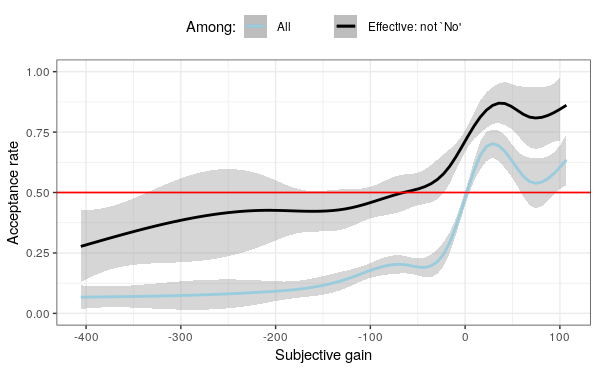
\includegraphics[width=0.7\columnwidth]{Images/WTP_Both.png}
{\footnotesize \parbox[t]{\textwidth}{\linespread{1.2}\selectfont \textsc{Note:} The black curve indicates that a majority of those who did not answer ``No'' to the question on the effectiveness of the policy accepted the reform when their subjective gain was above $-$60\euros{} per c.u. For the whole sample (blue curve), this majority acceptance is reached only when subjective gains are positive. This refers back to Section \ref{subsec:Survey-Beliefs-climate}.} \caption{Acceptance rate by subjective gain, informative of the willingness to pay for climate mitigation.\label{fig:WTP}}} %
\end{figure}

\section{Ensuring data quality (\emph{For online publication})}\label{app:speed} %

We took several steps to ensure the best possible data quality. We excluded the 4\% of respondents who spent less than 7 minutes on the full survey. We confirm that our main results are robust to choosing another cutoff than 7 minutes (see Table \ref{tab:7min}). In order to screen out inattentive respondents, a test for the quality of the responses was inserted, which asked respondents to select ``A little'' on a Likert scale. The 9\% of respondents who failed the test were also excluded, which yields a final sample of 3,002 respondents. Also, when the questions about a reform were spread over different pages, we recalled the details of the reform on each new page. We checked for careless or strange answers on numerical questions, such as income or the size of the household. We flagged 10 respondents with aberrant answers to the size of the household (and capped it to 12) and up to 273 respondents with inconsistent answers, such as a household income smaller than individual income, or a fuel economy higher than 90 liters per 100 km. Being flagged or having a low response time is not significantly correlated with our variables of interest such as policy support or subjective gain (the correlation is always from $-$1\% and 3\%). An examination of the flagged answers suggests that these respondents simply misunderstood the question. Among these inconsistent answers, 58 respondents have answered more than 10,000\euros{} as their monthly income (despite the word ``monthly'' being in bold and underlined), with answers in the typical range of French annual incomes. We have divided these figures by 12. 

\begin{table}[!htbp] \centering 
 \caption{Robustness of main results to the exclusion of poor quality answers.} 
 \label{tab:7min} 
\makebox[\textwidth][c]{ \begin{tabular}{@{\extracolsep{5pt}}lcccccc} 
\\[-1.8ex]\hline 
\hline \\[-1.8ex] 
\\[-1.2ex] & \multicolumn{3}{c}{Acceptance ($A^T$)} & \multicolumn{3}{c}{Correct updating ($U$)} \\[0.5ex]
& all & > 11 min & not flagged & all & > 11 min & not flagged \\ 
\hline \\[-1.0ex] 
Believes does not lose (.53) & 0.526 & 0.547 & 0.558 &  &  &  \\ 
 & (0.134) & (0.137) & (0.153) &  &  &  \\ 
 Winner, before feedback (.55) &  &  &  & 0.542 & 0.532 & 0.553 \\ 
 &  &  &  & (0.083) & (0.085) & (0.091) \\ 
 Initial tax: Approves (.18) &  &  &  & 0.180 & 0.213 & 0.197 \\ 
 &  &  &  & (0.046) & (0.049) & (0.049) \\ 
\hline \\[-1.0ex] 
Original regression: Table (column) & \ref{results_private_benefits} (1) & \ref{results_private_benefits} (1) & \ref{results_private_benefits} (1) & \ref{tab:heterogeneity_update} (2) & \ref{tab:heterogeneity_update} (2) & \ref{tab:heterogeneity_update} (2) \\ 
Effective F-statistic & 15.2 & 14.5 & 11.8 &  &  &  \\ 
Whole sample size & 2777 & 3165 & 2729 & 2777 & 3165 & 2729 \\ 
Observations & 1,978 & 1,825 & 1,826 & 1,370 & 1,261 & 1,242 \\ 
R$^{2}$ & 0.320 & 0.318 & 0.326 & 0.142 & 0.150 & 0.155 \\ 
\hline 
\hline \\[-0.8ex] 
\end{tabular} 
} {\footnotesize \parbox[t]{\textwidth}{\linespread{1.2}\selectfont \textsc{Note:} Two of our main results are checked on three alternative sampling restrictions: (1) inclusion of answers < 7 min, (2) exclusion of the 10\% of answers < 11 min, and (3) exclusion of flagged (inconsistent) respondents. Weights have been recalculated for each sample. The estimates on the original sample are reported next to variable name. See the original Tables for more details. The correlation between our main variables of interest and response time or being flagged is always below 3\%. Standard errors are reported in parentheses. This refers back to Section \ref{subsubsec:the-survey}.}}  \end{table}  


 \end{appendices}

\end{document}
